%% ======================================================================
%% REVISION (October 2026). Colour code:
%%   \new{...}   (blue)    new or rewritten text
%%   \torun{...} (magenta) numerical experiments for the authors to run
%%   \new{...}  (green)   language revision: rewritten for readability, same content
%%   \verify{...} (red margin note) point the authors should check
%%   Lines starting with "% REMOVED (rev):" are deleted text, kept as comments.
%% Previously coloured text (old blue/red revision marks) is now black.
%% Second pass (this version): the former green language revision is now
%% also blue; everything coloured blue is a change relative to the
%% submitted version.
%% Final version: \renewcommand{\new}[1]{#1}, \renewcommand{\verify}[1]{},
%% and delete all \torun blocks.
%% ======================================================================
\documentclass[11pt]{article}
\usepackage[margin=1in]{geometry}
\usepackage{amsmath,amssymb,amsthm,mathtools}
\usepackage[dvipsnames]{xcolor}
\usepackage{booktabs,enumitem,array,placeins}
\usepackage{graphicx}
\graphicspath{{figures/}}
\usepackage[colorlinks=true,linkcolor=blue!50!black,citecolor=blue!50!black]{hyperref}
\sloppy

% Set \numericsfalse to drop Section 6 (numerical verification) and Appendix B (code).
\newif\ifnumerics
\numericstrue

\newtheorem{theorem}{Theorem}
\newtheorem{lemma}{Lemma}
\newtheorem{proposition}{Proposition}
\theoremstyle{remark}\newtheorem{remark}{Remark}

\newcommand{\R}{\mathbb{R}}
\newcommand{\dd}{\mathrm{d}}
\newcommand{\Th}{\mathcal{T}_h}
\newcommand{\Vh}{V_h}\newcommand{\Qh}{Q_h}
\newcommand{\Vdiv}{V^{\mathrm{div}}}
\newcommand{\Vdivh}{V_h^{\mathrm{div}}}
\newcommand{\Dt}{D_t^{\mathrm{BDF2}}}
\newcommand{\tu}{\tilde u_h}
\newcommand{\Simex}{S_{\mathrm{IMEX}}}
\newcommand{\nrm}[1]{\|#1\|}
\newcommand{\Ph}{P_h}
\newcommand{\eps}{\varepsilon}
\theoremstyle{plain}
\newtheorem{corollary}{Corollary}
\newtheorem{assumption}{Assumption}
% ---- revision macros ----
\newcommand{\new}[1]{{\color{blue}#1}}
\newcommand{\torun}[1]{{\color{magenta}#1}}
\newcommand{\verify}[1]{\marginpar{\raggedright\tiny\color{red}#1}}
\setlength{\marginparwidth}{2.2cm}
\newenvironment{torunblock}{\par\color{magenta}}{\par}

\title{Pressure-Robust Error Estimates for a Stabilized BDF2--IMEX\\Navier--Stokes Scheme}
\author{%
Naveed Ahmed\thanks{Center for Applied Mathematics and Bioinformatics,
Department of Mathematics and Natural Sciences,
Gulf University for Science and Technology,
Mubarak Al-Abdullah Area/West Mishref, Kuwait.
Email: \texttt{ahmed.n@gust.edu.kw}.}
\and
Volker John\thanks{Weierstrass Institute for Applied Analysis and Stochastics (WIAS),
Anton-Wilhelm-Amo-Stra\ss e 39, 10117 Berlin, Germany;
and Freie Universit\"at Berlin, Department of Mathematics and Computer Science,
Arnimallee 6, 14195 Berlin, Germany.
Email: \texttt{john@wias-berlin.de}.}}
\date{September 20, 2026}

\begin{document}
\maketitle

\begin{abstract}
% REMOVED (rev): We analyse a fully discrete scheme for the incompressible Navier--Stokes equations that combines exactly divergence-free Scott--Vogelius elements on Alfeld splits, a three-term continuous interior penalty (CIP) stabilization of the convective derivative, and a linearly implicit BDF2 time discretization in which both the convective and the stabilizing transport fields are the second-order extrapolation $2u_h^n-u_h^{n-1}$. The scheme is unconditionally energy stable with a $\nu$-independent constant. For smooth solutions we prove a velocity error bound of order $\big((\nu+h)h^{2k}+\Delta t^4\big)^{1/2}$ whose constants are independent of the pressure and of inverse powers of the viscosity; in the convection-dominated regime $\nu\lesssim h$ this is $O(h^{k+1/2}+\Delta t^2)$. The proof is complete in two space dimensions and conditional on a potential-recovery property in three. The required a~priori $L^2$ bound on the discrete error is derived from a preliminary robust estimate rather than assumed. For the pressure we prove a robust but suboptimal bound of order $h^{k-1}+\Delta t^2/h$, and the optimal rate $h^k+\Delta t^2$ under an additional hypothesis on the discrete time derivative. Numerical experiments in two dimensions illustrate the analysis.
\new{We study a fully discrete method for the incompressible Navier--Stokes equations that combines exactly divergence-free Scott--Vogelius elements on Alfeld splits, a three-term continuous interior penalty (CIP) stabilization of the convective derivative, and a linearly implicit BDF2 scheme. Both the convective term and the stabilization use the extrapolated transport field $2u_h^n-u_h^{n-1}$, so each step requires one linear solve. The scheme is unconditionally energy stable, with a $\nu$-independent bound free of Gronwall factors. For smooth solutions the $L^2$ velocity error is of order $\big((\nu+h)h^{2k}+\Delta t^4\big)^{1/2}$, with constants independent of the pressure and of inverse powers of the viscosity; for $\nu\lesssim h$ this gives $O(h^{k+1/2}+\Delta t^2)$, the best $L^2$ rate known for $\nu$-independent bounds. The proof is complete in two dimensions for $k\in\{2,3\}$; in three dimensions it rests on a potential-recovery property that has not yet been established. The two-sided bounds on the extrapolated field needed by the normalized stabilization follow from a preliminary robust estimate under the mild condition $\Delta t\le c_0h^{1/2+\sigma}$, and a clamped normalization removes this condition from the velocity estimate. The pressure satisfies a robust bound of order $h^{k-1}+\Delta t^2/h$ in the discrete $\ell^2(L^2)$ norm. Numerical experiments in two dimensions, and with a simplified variant in three, confirm the rates and the robustness.}
\end{abstract}

\noindent\textbf{Keywords:} incompressible Navier--Stokes equations; pressure robustness; convection robustness; continuous interior penalty; Scott--Vogelius elements; BDF2; IMEX; error analysis.

\noindent\textbf{MSC (2020):} 65M12, 65M15, 65M60, 76D05.

%=====================================================================
\section{Introduction}\verify{New references [BH04, GLS19, Lin14, LM16, SV85]: check volume and page numbers.}
\new{%
Simulating incompressible flow at high Reynolds number remains hard for finite element methods, and two effects are largely responsible. The first comes from the way velocity and pressure are coupled. For classical inf-sup stable pairs such as Taylor--Hood, the velocity error bound contains the term $\nu^{-1}\inf_{q_h}\|p-q_h\|_0$. A large or complicated pressure can therefore spoil the velocity, even when the velocity itself is smooth \cite{JLMNR17,Lin14,LM16}. Methods whose velocity error does not see the pressure are called \emph{pressure robust}. The second effect is convection. Once $\nu$ is small compared with the mesh size, the Galerkin solution develops spurious oscillations, and the usual error bounds blow up through Gronwall factors such as $\exp(CT\nu^{-1})$ or through explicit powers of $\nu^{-1}$. We call a method \emph{convection robust} (or Reynolds robust) if its error constants contain no inverse powers of $\nu$. Why both properties matter in practice is discussed in \cite{GLS19,GJN21}.

Pressure robustness comes for free with exactly divergence-free elements. On Alfeld (barycentric) splits, the Scott--Vogelius pair \cite{SV85,AQ92,Zha05,GN18} produces discrete velocities that are divergence-free pointwise. If the error equation is tested with such a function, both the continuous and the discrete pressure drop out. Already the plain Galerkin method then gives $L^2$ velocity bounds of order $h^k$ that are robust with respect to both the pressure and $\nu$ \cite{SL17,GJN21}. To do better when convection dominates, some stabilization is needed; the best rate known for $\nu$-independent bounds is $h^{k+1/2}$ \cite{GJN21}. It was first proved for $H(\mathrm{div})$-conforming discontinuous Galerkin methods with upwinding \cite{GSS17,BBG20,HH21}. For $H^1$-conforming divergence-free elements, it has been obtained with a residual stabilization of the vorticity equation for the Oseen problem \cite{ABBGLM21} and with an SUPG-curl stabilization for the time-dependent Navier--Stokes equations \cite{BDV24}.

Continuous interior penalty (CIP) methods \cite{BH04,BFH06,BF07} stabilize by penalizing jumps of the convective derivative across interior faces. They are symmetric, they leave the velocity--pressure coupling untouched, and they need no residual of the strong equation. With divergence-free elements, however, the classical gradient-jump penalty is not enough for the $h^{k+1/2}$ rate. The reason lies in the consistency argument, which has to recover volume terms from face jumps in a space of potentials. Barrenechea, Burman, C\'aceres and Guzm\'an \cite{BBCG24} overcame this for the steady Oseen problem. Their three-term CIP form penalizes the jumps of $(\beta\cdot\nabla)u_h$, of $\nabla\times((\beta\cdot\nabla)u_h)$, and of the gradient of the latter. Combined with the $C^1$ Clough--Tocher potential space, it yields pressure- and convection-robust bounds of order $h^{k+1/2}$ in two dimensions. Garc\'ia-Archilla and Novo \cite{GAN25} then carried the method over to the semi-discrete Navier--Stokes equations, using the discrete velocity as transport field and normalizing the stabilization by $\|u_h\|_{0,\infty}^{-1}$.

What is still missing is a time discretization whose analysis does not bring back a dependence on $\nu^{-1}$ or on the pressure. A fully implicit scheme would require a nonlinear solve in every step, which is especially expensive here because the stabilization depends nonlinearly on the solution, both through its transport field and through its normalization. A linearly implicit BDF2 scheme avoids this. We replace the transport field by the second-order extrapolation $\tu^{n+1}=2u_h^n-u_h^{n-1}$, so that each step amounts to one linear system with a time-dependent matrix. Robust analyses of IMEX-BDF2 and BDF-$q$ schemes are available for grad-div stabilized methods \cite{GAN23,GAJN25}; they give $\nu$-robust bounds of order $h^k$. Space--time DG methods with $H(\mathrm{div})$-conforming velocities and upwinding were analysed in \cite{BDDG25}, and a Reynolds semi-robust hybrid method in \cite{BDDHR25}. Implicit--explicit multistep treatments of the CIP term itself are studied in \cite{BG20}.

\paragraph{Contribution.} In this paper we analyse the three-term CIP method of \cite{BBCG24,GAN25} with Scott--Vogelius elements and a linearly implicit BDF2--IMEX time discretization, in which both the convective term and the stabilization are evaluated with the extrapolated transport field $2u_h^n-u_h^{n-1}$. Our main results are as follows.
\begin{enumerate}[label=(\roman*),itemsep=2pt]
\item The scheme is unconditionally energy stable; the bound holds for every $\Delta t$, does not depend on $\nu$, and contains no Gronwall factor (Theorem~\ref{thm:stability}).
\item For $d=2$ and $k\in\{2,3\}$, the velocity error satisfies
\[
\|u(t_m)-u_h^m\|_0\le C\big((\nu+h)^{1/2}h^k+\Delta t^2\big),
\]
where $C$ depends neither on the pressure nor on $\nu^{-1}$ (Theorem~\ref{thm:velocity}). For $\nu\lesssim h$ this is $O(h^{k+1/2}+\Delta t^2)$, the fully discrete counterpart of \cite[Thm.~3.7]{GAN25}. In three dimensions the same estimate holds provided a potential-recovery property is available, which, as far as we know, has not been proved yet.
\item The normalized stabilization needs the extrapolated transport field to stay bounded from above and below. We obtain this from a preliminary robust estimate under the mild condition $\Delta t\le c_0h^{1/2+\sigma}$ (Corollary~\ref{cor:bootstrap}); with a clamped normalization, the condition is no longer needed for the velocity estimate (Remark~\ref{rem:clamp}).
\item For the pressure we prove a robust $\ell^2(L^2)$ bound of order $h^{k-1}+\Delta t^2/h$ (Theorem~\ref{thm:pressure}), and we indicate how the optimal rate could be reached (Remark~\ref{rem:optpressure}).
\end{enumerate}
Compared with \cite{GAN25}, the analysis needs two new ingredients. One is an estimate for the consistency error of the stabilization that is of order $h^{2k+1}$ uniformly in $\nu$ and does not feel the extrapolation defect $2u^n-u^{n-1}-u^{n+1}$ (Lemma~\ref{lem:stabilization-consistency}). The other is an induction over the time levels that keeps the extrapolated transport field bounded from above and below (Lemma~\ref{lem:prelim} and Corollary~\ref{cor:bootstrap}). The table below places our velocity estimate among related fully discrete, $\nu$-robust results ($k$: velocity degree; $\ell$: degree in time).
}

\begin{center}\small
\begin{tabular}{>{\raggedright\arraybackslash}p{2.4cm}>{\raggedright\arraybackslash}p{4.0cm}>{\raggedright\arraybackslash}p{3.5cm}>{\raggedright\arraybackslash}p{4.6cm}}\toprule
Reference & Space / time & Velocity bound & Time-step condition\\\midrule
\cite{GAJN25} (grad-div) & inf-sup stable / BDF-$q$ & $h^k+\Delta t^q$ & $\Delta t\,h^{-2}\le C$, $h^{-d/2}\Delta t^q\le C$\\
\cite{BDV24} & SUPG-curl, div-free / 2nd order & $\tau^2+h^{k+1/2}$ ($\nu\lesssim h$) & $\tau\lesssim h^{(s+2)/2}$ (asymptotic, $s\le4$)\\
\cite{BDDG25} & $H(\mathrm{div})$-DG / space--time DG & $\tau^{\ell+1}+\sqrt{\nu+h}\,h^k$ & $\tau\le C$\\
this paper & SV + CIP / BDF2--IMEX & $\Delta t^2+\sqrt{\nu+h}\,h^k$ & \new{$\Delta t\le c_0h^{1/2+\sigma}$ ($d=2$); none with clamping (Rem.~\ref{rem:clamp})}\\
\bottomrule\end{tabular}
\end{center}
\verify{Table, row [GAJN25]: check the condition $\Delta t\,h^{-2}\le C$ (it means $\Delta t\lesssim h^2$).}

\new{%
In the numerical part we test the Scott--Vogelius discretization, with and without the CIP stabilization, on a Taylor--Green vortex with manufactured forcing, on a three-dimensional travelling vortex, and on an under-resolved double shear layer; a Taylor--Hood discretization serves as a non-divergence-free reference in the pressure-robustness tests and where it is outperformed. The experiments measure the spatial rates predicted by the theory, confirm second-order accuracy in time, demonstrate the robustness with respect to $\nu$ and the pressure robustness of the divergence-free discretization, and show how the CIP terms suppress spurious oscillations.

\paragraph{Outline.} Section~\ref{sec:model} introduces the model problem and the spatially discrete CIP method. In Section~\ref{sec:bdf2} we formulate the BDF2--IMEX scheme, prove its energy stability, and derive the velocity error estimate. The pressure is treated in Section~\ref{sec:pressure}, and the numerical studies follow in Section~\ref{sec:numerics}. Appendix~A collects the estimate for the discrete time derivative used in the pressure bound.
}

%=====================================================================
\section{\new{Model problem and spatial discretization}}\label{sec:model}
\new{\subsection{Model problem}}
Let $\Omega\subset\R^d$, $d\in\{2,3\}$, be a bounded polyhedral Lipschitz domain, and let $T>0$. Given a viscosity $\nu>0$, a body force $f:(0,T]\times\Omega\to\R^d$, and an initial velocity $u_0$, the unknowns are the velocity field $u:(0,T]\times\Omega\to\R^d$ and the kinematic pressure $p:(0,T]\times\Omega\to\R$. The strong form of the model problem is
\begin{equation}\label{eq:strong-form}
\begin{aligned}
\partial_t u-\nu\Delta u+(u\cdot\nabla)u+\nabla p&=f &&\text{in }(0,T]\times\Omega,\\
\nabla\cdot u&=0 &&\text{in }(0,T]\times\Omega,\\
u&=0 &&\text{on }[0,T]\times\partial\Omega,\\
u(0)&=u_0 &&\text{in }\Omega.
\end{aligned}
\end{equation}
\new{The homogeneous Dirichlet condition models a no-slip wall.}

For the weak formulation, define
\[V=H_0^1(\Omega)^d,\qquad Q=L^2_0(\Omega)=\Big\{q\in L^2(\Omega):\int_\Omega q\,\dd x=0\Big\}.\]

Find $(u(t),p(t))\in V\times Q$, with $u(0)=u_0$, such that for all $(v,q)\in V\times Q$ and for almost every $t\in(0,T]$,
\begin{equation}\label{eq:weak-form}
\begin{aligned}
(\partial_tu,v)+\nu(\nabla u,\nabla v)+((u\cdot\nabla)u,v)-(p,\nabla\cdot v)&=(f,v),\\
(\nabla\cdot u,q)&=0.
\end{aligned}
\end{equation}
\new{Here $(\cdot,\cdot)$ is the $L^2(\Omega)$ inner product, and the pressure is sought in $L^2_0(\Omega)$ because it is determined only up to a constant. Testing only with divergence-free functions from}
\[V_{\mathrm{div}}=\{v\in H^1_0(\Omega)^d:\nabla\cdot v=0\},\]
\new{removes the pressure, and the velocity satisfies}
\begin{equation}\label{eq:div-free-weak-form}
(\partial_tu,v)+\nu(\nabla u,\nabla v)+((u\cdot\nabla)u,v)=(f,v)\qquad\forall v\in V_{\mathrm{div}}.
\end{equation}

% REMOVED (rev): \paragraph{Relation to the literature and contribution.} Pressure robustness of divergence-free mixed methods and its practical consequences are surveyed in \cite{JLMNR17}. For convection-dominated flows the best $L^2$ velocity rate that $\nu$-independent bounds deliver for smooth solutions is $O(h^{k+1/2})$; see the classification in \cite{GJN21}. With a pointwise divergence-free velocity, the unstabilized Galerkin method already gives pressure- and convection-robust $O(h^k)$ bounds \cite{SL17,GJN21}. The rate $O(h^{k+1/2})$ with pressure-robust bounds was first obtained for $H(\mathrm{div})$-conforming upwind discontinuous Galerkin methods \cite{GSS17,BBG20,HH21}, and for $H^1$-conforming divergence-free elements with a residual stabilization of the vorticity equation for the Oseen problem \cite{ABBGLM21}. The three-term CIP form used here was introduced and analysed for the steady Oseen problem in \cite{BBCG24}; its extension to the semi-discrete (continuous-in-time) Navier--Stokes equations, with the transport field replaced by the discrete velocity and normalized by $\|u_h\|_{0,\infty}^{-1}$, is due to \cite{GAN25}, whose analysis (the norm \eqref{eq:star-norm-definition}, the projection $w_h=\nabla\times\Ph z$, the comparison with the modified Stokes projection $s_h$) is followed closely below. A fully discrete pressure- and convection-robust $H^1$-conforming method, with an SUPG-curl stabilization, was analysed in \cite{BDV24}, with $\nu$-independent velocity bounds of order $O(\tau^2+h^{k+1/2})$ in the convection-dominated regime. Fully and semi-implicit space--time DG schemes with $H(\mathrm{div})$-conforming velocities and upwinding were shown to be pressure-robust and Reynolds semi-robust, with the same $(\nu+h)h^{2k}$ structure of the spatial error, in \cite{BDDG25}; a Reynolds-semirobust hybrid method with hybrid velocity and pressure is analysed in \cite{BDDHR25}. For CIP in the classical (not divergence-free) setting see \cite{BFH06,BF07}, for implicit--explicit multistep treatments of CIP terms see \cite{BG20}, and for robust analyses of IMEX-BDF2 and of BDF-$q$ schemes for the Navier--Stokes equations with grad-div stabilization see \cite{GAN23,GAJN25}; in the latter the robust velocity bound is of order $h^k$ in $L^2$ and is obtained under the conditions $h^{-d/2}\Delta t^q\le C$ and $\Delta t\,h^{-2}\le C$.

% REMOVED (rev): The contribution of this paper is a fully discrete analysis of the CIP scheme of \cite{BBCG24,GAN25} combined with the linearly implicit BDF2--IMEX time discretization, in which the transport field of both the convective term and the stabilization is the second-order extrapolation $2u_h^n-u_h^{n-1}$. The velocity estimate (Theorem~\ref{thm:velocity}) is the fully discrete analogue of \cite[Thm.~3.7]{GAN25}; the pressure estimate (Theorem~\ref{thm:pressure}) is robust but suboptimal, and optimal only under the additional hypothesis \eqref{eq:pressure-optimality-hypothesis} (Corollary~\ref{cor:pressure-optimal}). Compared with \cite{GAN25}, the new ingredients are the $G$-stability argument for BDF2 with an extrapolated transport field in both the convective and the stabilization terms, a stabilization-consistency estimate (Lemma~\ref{lem:stabilization-consistency}) that is insensitive to the extrapolation defect, and a fully discrete derivation of the a~priori bound \eqref{eq:bootstrap-bound} (Corollary~\ref{cor:bootstrap}). The only coupling of $\Delta t$ and $h$ is the mild condition $\Delta t\le c_0h$, which can be relaxed further (Remark~\ref{rem:timestep}). The following overview compares the velocity estimate with closely related fully discrete, $\nu$-robust results ($k$: velocity degree; $\ell$: degree in time).
% REMOVED (rev): 
% REMOVED (rev): \begin{center}\small
% REMOVED (rev): \begin{tabular}{>{\raggedright\arraybackslash}p{2.4cm}>{\raggedright\arraybackslash}p{4.0cm}>{\raggedright\arraybackslash}p{3.5cm}>{\raggedright\arraybackslash}p{4.6cm}}\toprule
% REMOVED (rev): Reference & Space / time & Velocity bound & Time-step condition\\\midrule
% REMOVED (rev): \cite{GAJN25} (grad-div) & inf-sup stable / BDF-$q$ & $h^k+\Delta t^q$ & $\Delta t\,h^{-2}\le C$, $h^{-d/2}\Delta t^q\le C$\\
% REMOVED (rev): \cite{BDV24} & SUPG-curl, div-free / 2nd order & $\tau^2+h^{k+1/2}$ ($\nu\lesssim h$) & $\tau\lesssim h^{(s+2)/2}$ (asymptotic, $s\le4$)\\
% REMOVED (rev): \cite{BDDG25} & $H(\mathrm{div})$-DG / space--time DG & $\tau^{\ell+1}+\sqrt{\nu+h}\,h^k$ & $\tau\le C$\\
% REMOVED (rev): this paper & SV + CIP / BDF2--IMEX & $\Delta t^2+\sqrt{\nu+h}\,h^k$ & $\Delta t\le c_0h$ (Rem.~\ref{rem:timestep})\\
% REMOVED (rev): \bottomrule\end{tabular}
% REMOVED (rev): \end{center}
% REMOVED (rev2): \new{The contribution of this paper is the fully discrete analysis of the CIP scheme of \cite{BBCG24,GAN25} combined with a linearly implicit BDF2--IMEX time discretization, in which the transport field of both the convective term and the stabilization is the second-order extrapolation $2u_h^n-u_h^{n-1}$. The velocity estimate (Theorem~\ref{thm:velocity}) is the fully discrete analogue of \cite[Thm.~3.7]{GAN25}; it is proved for $d=2$ and $k\in\{2,3\}$, and holds for $d=3$ conditionally on the potential-recovery property \eqref{eq:potential-recovery}. The pressure estimate (Theorem~\ref{thm:pressure}) is robust but loses one power of $h$; the route to the optimal rate is discussed in Remark~\ref{rem:optpressure}. Beyond \cite{GAN25}, the analysis requires a stabilization-consistency estimate that is uniform in $\nu$ and insensitive to the extrapolation defect (Lemma~\ref{lem:stabilization-consistency}), and a fully discrete two-sided $L^\infty$ bound on the extrapolated transport field (Corollary~\ref{cor:bootstrap}), which needs only $\Delta t\le c_0h^{1/2+\sigma}$. For a clamped normalization of the stabilization this condition can be removed from the velocity estimate (Remark~\ref{rem:clamp}).} The following overview compares the velocity estimate with closely related fully discrete, $\nu$-robust results ($k$: velocity degree; $\ell$: degree in time).
%=====================================================================
\new{\paragraph{Notation.} For a function $v$ of time we abbreviate $v^n:=v(t_n)$, so that $u^n=u(t_n)$, $p^n=p(t_n)$ and $f^n=f(t_n)$. We write $\|\cdot\|_0$ for the $L^2(\Omega)$ norm and $\|\cdot\|_{0,\infty}$ for the $L^\infty(\Omega)$ norm. For piecewise smooth functions, $(\cdot,\cdot)_h$ and $\|\cdot\|_{0,h}$ denote the elementwise (broken) $L^2$ inner product and norm over the triangulation, and $\|D^jv\|_{0,h}$ is the broken $L^2$ norm of all $j$-th order derivatives. For a family $\mathcal F$ of faces, $\|\varphi\|_{0,\mathcal F}^2=\sum_{F\in\mathcal F}\|\varphi\|_{0,F}^2$, and face-wise weights are written inside the norm, as in $\|h\varphi\|_{0,\mathcal F}$; since the meshes are quasi-uniform, we do not distinguish between the face size $h_F$ and $h$ in the estimates. Finally, $C$ denotes a generic constant that is independent of $h$, $\Delta t$, of $\nu\le\nu_{\max}$ and of the pressure, and may change from one occurrence to the next; dependencies that matter are stated explicitly.}

\subsection{Spatial discretization and stabilization}
Let $\Th$ be a shape-regular, quasi-uniform triangulation of $\Omega$, with mesh size $h$. We choose conforming finite element spaces $\Vh\subset H^1_0(\Omega)^d$ and $\Qh\subset L^2_0(\Omega)$ that satisfy the discrete inf-sup condition: there exists a constant $\beta>0$, independent of $h$, such that
\[\inf_{q_h\in\Qh}\sup_{v_h\in\Vh}\frac{(q_h,\nabla\cdot v_h)}{\|q_h\|_0\|\nabla v_h\|_0}\ge\beta.\]
Following the divergence-free setting from \cite{BBCG24,GAN25}, we also assume
\[\nabla\cdot\Vh\subset\Qh,\qquad \Vdivh=\{v_h\in\Vh:\nabla\cdot v_h=0\}.\]
A standard example is the Scott--Vogelius pair on barycentrically refined triangulations (Alfeld splits of a shape-regular, quasi-uniform triangulation),
\begin{align*}
\Vh=\{v_h\in H^1_0(\Omega)^d:v_h|_K\in P_k(K)^d\ \forall K\in\Th\},\\ 
\Qh=\{q_h\in L^2_0(\Omega):q_h|_K\in P_{k-1}(K)\ \forall K\in\Th\}.
\end{align*}
for suitable polynomial degree $k\ge d$ (so $k\ge2$ if $d=2$, $k\ge3$ if $d=3$); see \cite{AQ92} for $d=2$, \cite{Zha05} for $d=3$ and \cite{GN18} for general $d$. This choice gives pointwise divergence-free discrete velocities and hence pressure-robust velocity errors. \new{When this pair is used, $\Th$ stands for the refined (barycentric) triangulation itself; in particular, the set $\mathcal F_h^i$ of interior faces introduced below consists of the faces of the refined mesh, including those created by the splits, and $h$ is its mesh size.}

The semi-discrete problem reads: find $(u_h(t),p_h(t))\in\Vh\times\Qh$, with a suitable approximation $u_h(0)\approx u_0$, $u_h(0)\in\Vdivh$, such that for all $(v_h,q_h)\in\Vh\times\Qh$,
\begin{equation}\label{eq:sdp}
\begin{aligned}
(\partial_tu_h,v_h)+\nu(\nabla u_h,\nabla v_h)+((u_h\cdot\nabla)u_h,v_h)-(p_h,\nabla\cdot v_h)&=(f,v_h),\\
(\nabla\cdot u_h,q_h)&=0.
\end{aligned}
\end{equation}
Following the stabilized divergence-free approach in \cite{BBCG24}, extended to the Navier--Stokes equations in \cite{GAN25}, we introduce a continuous interior penalty (CIP) stabilization that penalizes jumps of convective derivatives over the interior mesh faces. Let $\mathcal F_h^i$ denote the set of interior faces. For each $F=\partial K^+\cap\partial K^-\in\mathcal F_h^i$, fix a unit normal $n_F$ directed from $K^+$ to $K^-$. If $w^\pm$ denotes the trace on $F$ from $K^\pm$, define the jump componentwise by
\[
[\![w]\!]_F:=w^+-w^-.
\]
In the following, we write $n=n_F$ and suppress the subscript $F$ on the jump. %Reversing the orientation changes the sign of each jump but leaves all products of two jumps unchanged. 
On each element $K$, define the elementwise operator
\[(Bw)|_K=\nabla\times((u_h\cdot\nabla)w)|_K.\]
For non-dimensional stabilization parameters $\delta_1,\delta_2,\delta_3>0$, the stabilization term $S$ is defined by
\[S(u_h,v_h)=\|u_h\|_{0,\infty}^{-1}\sum_{j=1}^3\delta_jS_j(u_h,v_h)\quad(\text{with }S:=0\text{ if }\|u_h\|_{0,\infty}=0),\]
where
\begin{align*}
S_1(u_h,v_h)&=\sum_{F\in\mathcal F_h^i}\int_F h_F^2\,[\![(u_h\cdot\nabla)u_h\times n]\!]\cdot[\![(u_h\cdot\nabla)v_h\times n]\!]\,\dd s,\\
S_2(u_h,v_h)&=\sum_{F\in\mathcal F_h^i}\int_F h_F^4\,[\![Bu_h]\!]\cdot[\![Bv_h]\!]\,\dd s,\\
S_3(u_h,v_h)&=\sum_{F\in\mathcal F_h^i}\int_F h_F^6\,[\![\nabla Bu_h]\!]:[\![\nabla Bv_h]\!]\,\dd s.
\end{align*}
Thus the CIP-stabilized semidiscrete problem is: find $(u_h(t),p_h(t))\in\Vh\times\Qh$ such that
\begin{equation}\label{eq:sdp-stab}
\begin{aligned}
(\partial_tu_h,v_h)+\nu(\nabla u_h,\nabla v_h)+((u_h\cdot\nabla)u_h,v_h)+S(u_h,v_h)-(p_h,\nabla\cdot v_h)&=(f,v_h),\\
(\nabla\cdot u_h,q_h)&=0,
\end{aligned}
\end{equation}
for all $(v_h,q_h)\in\Vh\times\Qh$. Compared with \eqref{eq:sdp}, the role of $S$ in \eqref{eq:sdp-stab} is to add streamline dissipation through interelement jump terms while preserving the pressure-robust structure of the divergence-free finite element method.
By trace and inverse inequalities, for a transport field $\tilde u\in\Vh$ and $v_h\in\Vh$ one has
\begin{equation}\label{eq:raw-cip-continuity}
S_j(v_h,v_h)\le C\,h\,\|\tilde u\|_{0,\infty}^2\|\nabla v_h\|_0^2
\end{equation}
with $C$ depending on the trace and inverse-inequality constants (for $S_2,S_3$ through $\|\nabla^m\tilde u\|_{0,\infty}\le Ch^{-m}\|\tilde u\|_{0,\infty}$, $m=1,2$) and the shape regularity. This is a bound on the \emph{raw}, unnormalized form $S_j$ as defined above; two powers of $\|\tilde u\|_{0,\infty}$ appear because $\tilde u$ occurs twice inside the jump operators ($S_1$ directly, $S_2,S_3$ through $B$). Dividing \eqref{eq:raw-cip-continuity} by $\|\tilde u\|_{0,\infty}$, as the scheme does, gives the normalized bound actually used below and in Section~\ref{sec:pressure}:
\begin{equation}\label{eq:cip-continuity}
\|\tilde u\|_{0,\infty}^{-1}S_j(v_h,v_h)\le C\,h\,\|\tilde u\|_{0,\infty}\,\|\nabla v_h\|_0^2,
\qquad\text{hence}\qquad
\Simex^{n+1}(v_h,v_h)\le C\,h\,\|\tu^{n+1}\|_{0,\infty}\,\|\nabla v_h\|_0^2.
\end{equation}
The normalized estimate \eqref{eq:cip-continuity} is an upper bound and is used in the stabilization-residual estimate in the pressure-error proof.
The stabilization-consistency estimate (Lemma~\ref{lem:stabilization-consistency}) divides face terms that are \emph{not} proportional to $\|\tilde u\|_{0,\infty}^2$ by $\|\tilde u\|_{0,\infty}$ and therefore needs a \emph{lower} bound on $\|\tilde u\|_{0,\infty}$, see Assumption~\ref{ass:lower} and \cite[(48)]{GAN25}. As suggested in \cite[Remark~3.4]{GAN25}, this can also be enforced in the scheme by replacing $\|\tilde u\|_{0,\infty}^{-1}$ with $\max(u_{\min},\|\tilde u\|_{0,\infty})^{-1}$ for a fixed $u_{\min}>0$, the proofs below apply to that variant with only notational changes\new{; a two-sided clamp, which also removes the need for an upper bound, is discussed in Remark~\ref{rem:clamp}}.

%=====================================================================
\section{BDF2--IMEX time discretization\new{ and velocity error analysis}}\label{sec:bdf2}
We now discretize the stabilized semidiscrete problem~\eqref{eq:sdp-stab} in time. Let $0=t_0<t_1<\dots<t_N=T$ be a uniform partition of $[0,T]$, with time step $\Delta t=t_n-t_{n-1}$. For a sequence $\{w^n\}_{n=0}^N$, the BDF2 approximation of the time derivative at $t_{n+1}$ is
\[
    \Dt w^{n+1}
    :=\frac{3w^{n+1}-4w^n+w^{n-1}}{2\Delta t}.
\]
To obtain a linear problem at each time step, the nonlinear convective velocity is treated explicitly by the second-order extrapolation
\[
    \tu^{n+1}=2u_h^n-u_h^{n-1}.
\]
The viscous term, pressure term, incompressibility constraint, and 
test-function factor in the convection operator are treated implicitly. This 
gives an implicit--explicit (IMEX) BDF2 method. Given $(u_h^n,p_h^n)$ and 
$(u_h^{n-1},p_h^{n-1})$, find $(u_h^{n+1},p_h^{n+1})\in\Vh\times\Qh$ such that 
for all $(v_h,q_h)\in\Vh\times\Qh$,
\begin{equation}\label{eq:fully-discrete-scheme}
\begin{aligned}
(\Dt u_h^{n+1},v_h)+\nu(\nabla u_h^{n+1},\nabla v_h)+((\tu^{n+1}\cdot\nabla)u_h^{n+1},v_h)+\Simex^{n+1}(u_h^{n+1},v_h)&\\
-(p_h^{n+1},\nabla\cdot v_h)&=(f^{n+1},v_h),\\
(\nabla\cdot u_h^{n+1},q_h)&=0.
\end{aligned}
\end{equation}
Here $f^{n+1}=f(t_{n+1})$. The IMEX version of the CIP stabilization is formed with the same extrapolated transport field. On each element $K$, define
\[(B^{n+1}_{\mathrm{IMEX}}w)|_K=\nabla\times((\tu^{n+1}\cdot\nabla)w)|_K.\]
Then
\[\Simex^{n+1}(u_h^{n+1},v_h)=\|\tu^{n+1}\|_{0,\infty}^{-1}\sum_{j=1}^3\delta_jS^{n+1}_{j,\mathrm{IMEX}}(u_h^{n+1},v_h),\]
with the convention $\Simex^{n+1}:=0$ whenever $\|\tu^{n+1}\|_{0,\infty}=0$, and
\begin{align*}
S^{n+1}_{1,\mathrm{IMEX}}(u_h^{n+1},v_h)&=\sum_{F}\int_F h_F^2[\![(\tu^{n+1}\cdot\nabla)u_h^{n+1}\times n]\!]\cdot[\![(\tu^{n+1}\cdot\nabla)v_h\times n]\!]\dd s,\\
S^{n+1}_{2,\mathrm{IMEX}}(u_h^{n+1},v_h)&=\sum_{F}\int_F h_F^4[\![B^{n+1}_{\mathrm{IMEX}}u_h^{n+1}]\!]\cdot[\![B^{n+1}_{\mathrm{IMEX}}v_h]\!]\dd s,\\
S^{n+1}_{3,\mathrm{IMEX}}(u_h^{n+1},v_h)&=\sum_{F}\int_F h_F^6[\![\nabla B^{n+1}_{\mathrm{IMEX}}u_h^{n+1}]\!]:[\![\nabla B^{n+1}_{\mathrm{IMEX}}v_h]\!]\dd s.
\end{align*}
Thus, at each time level, the convective coefficients and stabilization weights 
are known from previous time levels, while $u_h^{n+1}$ and $p_h^{n+1}$ are 
computed implicitly. Since BDF2 is a two-step method, the first value $u_h^1$ 
can be obtained by a first-order IMEX Euler step or by another consistent 
one-step starter.

%=====================================================================
\subsection{Stability of the fully discrete scheme}
We now state a basic energy stability estimate for the fully discrete BDF2--IMEX scheme~\eqref{eq:fully-discrete-scheme}. For notational convenience, define
\[c(w;u,v)=((w\cdot\nabla)u,v),\qquad\tu^{n+1}=2u_h^n-u_h^{n-1}.\]
Since the scheme enforces $(\nabla\cdot u_h^j,q_h)=0$ for all $q_h\in\Qh$, the extrapolated velocity $\tu^{n+1}$ is also discretely divergence-free \emph{provided the starting value $u_h^0$ is also in $\Vdivh$} (e.g.\ the modified Stokes projection of $u_0$; a nodal interpolant of $u_0$ is not divergence-free). In the exactly divergence-free Scott--Vogelius setting, this implies $\nabla\cdot\tu^{n+1}=0$ pointwise.

% REMOVED (rev): \begin{lemma}
% REMOVED (rev): \label{lem:nonlin}
% REMOVED (rev): For sufficiently smooth vector fields $w,u\in H^1_0(\Omega)^d$,
% REMOVED (rev): \[c(w;u,u)=-\frac12((\nabla\cdot w)u,u).\]
% REMOVED (rev): Consequently,
% REMOVED (rev): \[|c(w;u,u)|\le\frac12\|\nabla\cdot w\|_{0,\infty}\|u\|_0^2\le\frac{\sqrt d}2\|\nabla w\|_{0,\infty}\|u\|_0^2.\]
% REMOVED (rev): In particular, if $\nabla\cdot w=0$, then $c(w;u,u)=0$.
% REMOVED (rev): \end{lemma}
% (Lemma on skew-symmetry removed; it is standard, see \cite{GR86,Joh16}.)

% REMOVED (rev): \begin{theorem}\label{thm:stability}
% REMOVED (rev): Assume that the velocity space is exactly divergence-free, that the no-slip boundary condition is imposed strongly, that $u_h^0,u_h^1\in\Vdivh$ (so that $\nabla\cdot\tu^{n+1}=0$ for all $n\ge1$), and that $f^{n+1}\in L^2(\Omega)^d$. There is a number $\Delta t_0>0$, independent of $\nu$, such that for $\Delta t\le\Delta t_0$ and every $m\ge2$, the solution of \eqref{eq:fully-discrete-scheme} satisfies
% REMOVED (rev): \begin{multline}\label{eq:fdp_stability}
% REMOVED (rev): \|u_h^m\|_0^2+\|2u_h^m-u_h^{m-1}\|_0^2
% REMOVED (rev): +\nu\Delta t\sum_{n=1}^{m-1}\|\nabla u_h^{n+1}\|_0^2
% REMOVED (rev): +\Delta t\sum_{n=1}^{m-1}\Simex^{n+1}(u_h^{n+1},u_h^{n+1})\\
% REMOVED (rev): \le C_T\left(\|u_h^1\|_0^2+\|2u_h^1-u_h^0\|_0^2
% REMOVED (rev): +\Delta t\sum_{n=1}^{m-1}\|f^{n+1}\|_0^2\right),
% REMOVED (rev): \end{multline}
% REMOVED (rev): where $C_T$ depends on the final time through a discrete Gronwall factor. 
% REMOVED (rev): \end{theorem}
% REMOVED (rev): 
% REMOVED (rev): \begin{proof}
% REMOVED (rev): Choose $v_h=u_h^{n+1}$ in the momentum equation of the fully discrete scheme \eqref{eq:fully-discrete-scheme} and choose $q_h=p_h^{n+1}$ in the incompressibility equation. The pressure term vanishes because $(p_h^{n+1},\nabla\cdot u_h^{n+1})=0$. The BDF2 term is treated using the identity
% REMOVED (rev): \[(3a-4b+c,a)=\frac12\big(\|a\|_0^2+\|2a-b\|_0^2-\|b\|_0^2-\|2b-c\|_0^2+\|a-2b+c\|_0^2\big)\]
% REMOVED (rev): with $a=u_h^{n+1}$, $b=u_h^n$, and $c=u_h^{n-1}$. Hence
% REMOVED (rev): \[
% REMOVED (rev): (\Dt u_h^{n+1},u_h^{n+1})=\frac1{4\Delta t}\big(F^{n+1}-F^n+D^{n+1}\big),
% REMOVED (rev): \]
% REMOVED (rev): where
% REMOVED (rev): \[
% REMOVED (rev): F^{n+1}=\|u_h^{n+1}\|_0^2+\|2u_h^{n+1}-u_h^n\|_0^2,
% REMOVED (rev): \qquad
% REMOVED (rev): D^{n+1}=\|u_h^{n+1}-2u_h^n+u_h^{n-1}\|_0^2\ge0.
% REMOVED (rev): \]
% REMOVED (rev): The viscous term gives $\nu\|\nabla u_h^{n+1}\|_0^2$ and  the CIP term is nonnegative because it is a weighted sum of squared face-jump seminorms: $$\Simex^{n+1}(u_h^{n+1},u_h^{n+1})\ge0.$$
% REMOVED (rev):  For the IMEX convection term, apply the Lemma~\ref{lem:nonlin} with $w=\tu^{n+1}$ and $u=u_h^{n+1}$. Since the extrapolated velocity is exactly divergence-free in the Scott--Vogelius setting, $\nabla\cdot\tu^{n+1}=0$, and therefore $c(\tu^{n+1};u_h^{n+1},u_h^{n+1})=0$. Finally, Cauchy--Schwarz and Young's inequality in $L^2(\Omega)$ give
% REMOVED (rev): \[
% REMOVED (rev): (f^{n+1},u_h^{n+1})
% REMOVED (rev): \le\frac12\|f^{n+1}\|_0^2+\frac12\|u_h^{n+1}\|_0^2
% REMOVED (rev): \le\frac12\|f^{n+1}\|_0^2+\frac12F^{n+1}.
% REMOVED (rev): \]
% REMOVED (rev): Combining the preceding identities and multiplying by $4\Delta t$ gives
% REMOVED (rev): \begin{equation}\label{eq:nu-independent-stability-step}
% REMOVED (rev): F^{n+1}-F^n+D^{n+1}
% REMOVED (rev): +4\Delta t\left(\nu\|\nabla u_h^{n+1}\|_0^2
% REMOVED (rev): +\Simex^{n+1}(u_h^{n+1},u_h^{n+1})\right)
% REMOVED (rev): \le2\Delta t\|f^{n+1}\|_0^2+2\Delta t F^{n+1}.
% REMOVED (rev): \end{equation}
% REMOVED (rev): Discarding $D^{n+1}\ge0$ and taking $\Delta t\le\Delta t_0:=1/4$, set
% REMOVED (rev): \[
% REMOVED (rev): \alpha=(1-2\Delta t)^{-1}.
% REMOVED (rev): \]
% REMOVED (rev): Then \eqref{eq:nu-independent-stability-step} implies
% REMOVED (rev): \[
% REMOVED (rev): F^{n+1}+4\alpha\Delta t\left(\nu\|\nabla u_h^{n+1}\|_0^2
% REMOVED (rev): +\Simex^{n+1}(u_h^{n+1},u_h^{n+1})\right)
% REMOVED (rev): \le\alpha F^n+2\alpha\Delta t\|f^{n+1}\|_0^2.
% REMOVED (rev): \]
% REMOVED (rev): Iterating this inequality from $n=1$ to $m-1$ yields
% REMOVED (rev): \[
% REMOVED (rev): \begin{aligned}
% REMOVED (rev): F^m
% REMOVED (rev): &+4\alpha\Delta t\sum_{n=1}^{m-1}\alpha^{m-1-n}
% REMOVED (rev):   \nu\|\nabla u_h^{n+1}\|_0^2\\
% REMOVED (rev): &+4\alpha\Delta t\sum_{n=1}^{m-1}\alpha^{m-1-n}
% REMOVED (rev):   \Simex^{n+1}(u_h^{n+1},u_h^{n+1})\\
% REMOVED (rev): &\le\alpha^{m-1}F^1\\
% REMOVED (rev): &\quad+2\alpha\Delta t\sum_{n=1}^{m-1}\alpha^{m-1-n}\|f^{n+1}\|_0^2.
% REMOVED (rev): \end{aligned}
% REMOVED (rev): \]
% REMOVED (rev): For $\Delta t\le1/4$, $\alpha\le e^{4\Delta t}$, and therefore $\alpha^{m-1}\le e^{4T}$. Since every weight $\alpha^{m-1-n}$ is at least one, the unweighted accumulated dissipations on the left are also controlled. Absorbing the fixed numerical factors into $C_T$ proves the assertion. 
% REMOVED (rev): %with for example $C_T=C e^{4T}$, independently of $\nu$.
% REMOVED (rev): \end{proof}
\begin{theorem}\label{thm:stability}
Assume that the velocity space is exactly divergence-free, that the no-slip boundary condition is imposed strongly, that $u_h^0,u_h^1\in\Vdivh$ (so that $\nabla\cdot\tu^{n+1}=0$ for all $n\ge1$), and that $f^{n+1}\in L^2(\Omega)^d$. \new{Then, for every $\Delta t>0$ and every $m\ge2$,} the solution of \eqref{eq:fully-discrete-scheme} satisfies
\begin{multline}\label{eq:fdp_stability}
\|u_h^m\|_0^2+\|2u_h^m-u_h^{m-1}\|_0^2
+\new{4}\nu\Delta t\sum_{n=1}^{m-1}\|\nabla u_h^{n+1}\|_0^2
+\new{4}\Delta t\sum_{n=1}^{m-1}\Simex^{n+1}(u_h^{n+1},u_h^{n+1})\\
\le\new{3\big(\|u_h^1\|_0^2+\|2u_h^1-u_h^0\|_0^2\big)+18\Big(\Delta t\sum_{n=1}^{m-1}\|f^{n+1}\|_0\Big)^2.}
\end{multline}
\new{The bound holds without restriction on $\Delta t$, contains no Gronwall factor, and is independent of $\nu$.}
\end{theorem}

\begin{proof}
Choose $v_h=u_h^{n+1}$ and $q_h=p_h^{n+1}$ in \eqref{eq:fully-discrete-scheme}; the pressure term vanishes because $(p_h^{n+1},\nabla\cdot u_h^{n+1})=0$. \new{By the $G$-stability identity of BDF2 (see, e.g., \cite[Sec.~V.6]{HW96} or \cite{GAN23})}
\[(3a-4b+c,a)=\frac12\big(\|a\|_0^2+\|2a-b\|_0^2-\|b\|_0^2-\|2b-c\|_0^2+\|a-2b+c\|_0^2\big),\]
with $a=u_h^{n+1}$, $b=u_h^n$, $c=u_h^{n-1}$, one has
\[
(\Dt u_h^{n+1},u_h^{n+1})=\frac1{4\Delta t}\big(F^{n+1}-F^n+D^{n+1}\big),\qquad
F^{n+1}=\|u_h^{n+1}\|_0^2+\|2u_h^{n+1}-u_h^n\|_0^2,
\]
with $D^{n+1}=\|u_h^{n+1}-2u_h^n+u_h^{n-1}\|_0^2\ge0$. The CIP term is nonnegative, and \new{$c(\tu^{n+1};u_h^{n+1},u_h^{n+1})=0$ because $\nabla\cdot\tu^{n+1}=0$ and $u_h^{n+1}\in H^1_0(\Omega)^d$ \cite{GR86,Joh16}}. \new{Bounding $(f^{n+1},u_h^{n+1})\le\|f^{n+1}\|_0(F^{n+1})^{1/2}$ and multiplying by $4\Delta t$ gives
\[
F^{n+1}-F^n+4\Delta t\big(\nu\|\nabla u_h^{n+1}\|_0^2+\Simex^{n+1}(u_h^{n+1},u_h^{n+1})\big)\le4\Delta t\,\|f^{n+1}\|_0\,(F^{n+1})^{1/2}.
\]
Sum from $n=1$ to $m-1$ and write $A_m:=\Delta t\sum_{n=1}^{m-1}\|f^{n+1}\|_0$ and $M_m:=\max_{1\le j\le m}F^j$:
\begin{equation}\label{eq:stab-sum}
F^m+4\Delta t\sum_{n=1}^{m-1}\big(\nu\|\nabla u_h^{n+1}\|_0^2+\Simex^{n+1}(u_h^{n+1},u_h^{n+1})\big)\le F^1+4A_mM_m^{1/2}.
\end{equation}
Applying \eqref{eq:stab-sum} at an index $j\le m$ with $F^j=M_m$ and using $A_j\le A_m$ gives $M_m\le F^1+4A_mM_m^{1/2}$, hence $M_m^{1/2}\le2A_m+(4A_m^2+F^1)^{1/2}\le(F^1)^{1/2}+4A_m$. Inserting this into \eqref{eq:stab-sum} and using $4A_m(F^1)^{1/2}\le2F^1+2A_m^2$ proves \eqref{eq:fdp_stability}.}
\end{proof}

% REMOVED (rev): \begin{remark}\label{rem:nondivfree}
% REMOVED (rev): If one uses an inf-sup stable pair that is not pointwise divergence-free,
% REMOVED (rev): Theorem~\ref{thm:stability} is no longer available as stated. There are two options:
% REMOVED (rev): \begin{itemize}
% REMOVED (rev):     \item replace the convection term by the skew-symmetric form $\frac12 c(\tilde u;u,v)-\frac12 c(\tilde u;v,u)$, which vanishes for $v=u$ for any $\tilde u$ with $\tilde u\cdot n=0$ on $\partial\Omega.$
% REMOVED (rev):     %this is a different scheme from \eqref{eq:fully-discrete-scheme}.
% REMOVED (rev):     \item or bound
% REMOVED (rev): \[
% REMOVED (rev): \frac12((\nabla\cdot\tilde u_h)u,u)\le\frac12\|\nabla\cdot\tilde u_h\|_{0,\infty}\|u\|_0^2
% REMOVED (rev): \]
% REMOVED (rev): this yields a discrete Gronwall factor $\exp(CT\max_n\|\nabla\cdot\tilde u_h^{n}\|_{0,\infty})$, together with the mild, solution-dependent step restriction $\Delta t\,\max_n\|\nabla\cdot\tilde u_h^{n}\|_{0,\infty}\le c<1$ needed to absorb the implicit term, and requires an a~priori bound on the discrete divergence of the extrapolated velocity.
% REMOVED (rev): \end{itemize}
% REMOVED (rev): \end{remark}
% (Remark on pairs that are not divergence-free removed: outside the scope of the paper.)

%=====================================================================
% \section{Error analysis}\label{sec:error}
In the following, the divergence-free structure is used to remove pressure from the velocity estimate, while the CIP terms control convective derivatives through interelement jumps.

\subsection{Approximation assumptions and projections}\label{subsec:approx}
Assume that the exact solution is sufficiently regular, for example
\[u\in L^\infty(0,T;H^{k+1}(\Omega)^d),\qquad\partial_tu\in L^2(0,T;H^{k+1}(\Omega)^d),\]
and, for the viscosity-independent treatment of the temporal residuals, assume explicitly that
\[
    \partial_{tt}u\in L^\infty(0,T;L^2(\Omega)^d),\qquad
\partial_{ttt}u\in L^2(0,T;L^2(\Omega)^d).
\]
% REMOVED (rev): Assume also that the potential $z$ satisfying $\nabla\times z=u$ has the regularity required by the potential-space projection used in the CIP analysis. The domain is assumed simply connected (and, if $d=3$, to have a connected boundary), so that a potential $z$ with $\nabla\times z=u$ exists. For contractible Lipschitz domains, $\|z\|_{H^{r+1}}\le C\|u\|_{H^r}$ \cite{CM10}. Following \cite{BBCG24,GAN25}, we use the following structural assumptions:
\new{For $d=2$ and $\Omega$ simply connected, a divergence-free $u\in H^1_0(\Omega)^2$ has a stream function $z\in H^2_0(\Omega)$ with $\nabla\times z=u$, unique up to a constant; since $\nabla z$ is a rotation of $u$, $\|z\|_{H^{r+1}}\le C\|u\|_{H^r}$ holds without any elliptic regularity. For $d=3$ one needs, in addition, a vector potential with boundary conditions that put $\nabla\times\Ph z$ in $H^1_0(\Omega)^3$, together with the corresponding regularity; see \cite{GR86,CM10}.} Following \cite{BBCG24,GAN25}, we use the following structural assumptions:
\begin{enumerate}[label=\arabic*.,itemsep=1pt]
\item $\nabla\cdot\Vh\subset\Qh$, so the discrete velocity can be exactly divergence-free.
\item The pair $(\Vh,\Qh)$ is inf-sup stable.
\item There exists a potential space $Z_h\subset Z$ such that $\nabla\times Z_h=\Vdivh$.
\item If $\Ph:Z\to Z_h$ is the $L^2$-projection, then for $|\alpha|\le\min(5,k+2)$,
\[\|h^{|\alpha|}\partial^\alpha(z-\Ph z)\|_{0,h}\le Ch^{k+2}\|z\|_{H^{k+2}}.\]
% REMOVED (rev): In \cite{BBCG24,GAN25} this is assumed for $|\alpha|\le k+1$; the case $|\alpha|=k+2$ follows from the case $\alpha=0$, an inverse inequality and an optimal quasi-interpolant into $Z_h$. For $d=2$ and Alfeld splits it is proved in \cite[Sec.~4]{BBCG24} for quasi-uniform meshes.
In \cite{BBCG24,GAN25} this is assumed for $|\alpha|\le k+1$; \new{the case $|\alpha|=k+2$ is immediate, since $\Ph z$ is piecewise polynomial of degree $k+1$, so that $\partial^\alpha\Ph z=0$ elementwise.} For $d=2$ and Alfeld splits it is proved in \cite[Sec.~4]{BBCG24} for quasi-uniform meshes.
\item The potential space has the following recovery property. For every broken
polynomial $\chi_h$ in the range of the elementwise operator used below,
\begin{equation}\label{eq:potential-recovery}
\inf_{m_h\in Z_h}\|h^{3/2}(\chi_h-m_h)\|_{0,h}
\le C\left(\|h^2[\![\chi_h]\!]\|_{0,\mathcal F_h^i}
+\|h^3[\![\nabla\chi_h]\!]\|_{0,\mathcal F_h^i}\right).
\end{equation}
This is the discrete potential-recovery assumption corresponding to the two
additional penalties $S_2$ and $S_3$; it is the step that converts their face
jumps into control of a broken volume term.
% REMOVED (rev): \textcolor{blue}{For Scott--Vogelius elements on Alfeld (Clough--Tocher) splits, with $Z_h$ the $C^1$ Clough--Tocher space of degree $k+1$, \eqref{eq:potential-recovery} is proved in \cite[Lemma~4.1]{BBCG24} for $d=2$ and for broken polynomials $\chi_h$ of degree $\le k+1$ on the refined mesh. For $d=3$ (potential spaces from \cite{FGN20}) it is, to our knowledge, not proved; \cite[Sec.~6]{BBCG24} states that the proof can be extended. \textbf{Hence every result below that uses \eqref{eq:potential-recovery} (Lemma~\ref{lem:nonlinear-residual}, Theorems~\ref{thm:velocity} and \ref{thm:pressure}) is proved for $d=2$, and is conditional on \eqref{eq:potential-recovery} for $d=3$.} The degree restriction is the reason for the auxiliary transport field $\beta_0$ in the proof of Lemma~\ref{lem:nonlinear-residual}.}
% REMOVED (rev): \end{enumerate}
For Scott--Vogelius elements on Alfeld (Clough--Tocher) splits, with $Z_h$ the $C^1$ Clough--Tocher space of degree $k+1$, \eqref{eq:potential-recovery} is proved in \cite[Lemma~4.1]{BBCG24} for $d=2$ and for broken polynomials $\chi_h$ of degree $\le k+1$ on the refined mesh. For $d=3$ (potential spaces from \cite{FGN20}) it is, to our knowledge, not proved; \cite[Sec.~6]{BBCG24} states that the proof can be extended.
\end{enumerate}

\new{\paragraph{Scope of the error analysis.} From here on we restrict the error analysis to $d=2$ and $k\in\{2,3\}$. The reason is the recovery step: for these degrees, with $\beta=\tu^{n+1}$ and $e\in\Vh$, the function $\nabla\times((\beta\cdot\nabla)e)$ is elementwise a polynomial of degree $2k-2\le k+1$, so \eqref{eq:potential-recovery} can be applied to it directly, without an auxiliary low-order transport field (Lemma~\ref{lem:nonlinear-residual}). Higher degrees could be handled by inserting a piecewise constant Raviart--Thomas approximation of the transport field as in \cite{BBCG24}, at the cost of an additional a~priori $L^2$ bound on the discrete error; we do not pursue this here. In three dimensions, where $k=3$, everything below carries over as soon as \eqref{eq:potential-recovery} is available for the potential spaces of \cite{FGN20} and assumption~4 holds for the associated $L^2$-projection.}
Define the divergence-free projected velocity
\[w_h(t)=\nabla\times\Ph z(t)\in\Vdivh.\]
Then, for smooth solutions,
\[\|u(t)-w_h(t)\|_0+h\|\nabla(u(t)-w_h(t))\|_0\le Ch^{k+1}\|u(t)\|_{H^{k+1}}.\]
Use the modified Stokes projection $s_h\in\Vdivh$, characterized by
\[(\nabla s_h,\nabla\varphi_h)=(\nabla u,\nabla\varphi_h)\qquad\forall\varphi_h\in\Vdivh,\]
which satisfies
\[\|s_h-u\|_0+h\|\nabla(s_h-u)\|_0\le Ch^{k+1}\|u\|_{H^{k+1}}.\]
The pointwise bounds
\begin{equation}
    \|w_h\|_{0,\infty}\le C\|u\|_{0,\infty}+Ch^{k+1-d/2}\|z\|_{H^{k+2}},\qquad\|\nabla w_h\|_{0,\infty}\le C\|\nabla u\|_{0,\infty}+Ch^{k-d/2}\|z\|_{H^{k+2}}
\end{equation}
are used to keep the convective constants independent of inverse powers of the viscosity.

% \subsection{Error splitting}
At each time level, write
\[u(t_n)-u_h^n=\eta^n-e_h^n,\qquad\eta^n=u(t_n)-w_h^n,\qquad e_h^n=u_h^n-w_h^n.\]
The approximation part $\eta^n$ is controlled by the projection estimates, while the discrete part $e_h^n$ is controlled by an energy argument. Since both $u_h^n$ and $w_h^n$ are discretely divergence-free, we have $e_h^n\in\Vdivh$. This is the key pressure-robustness mechanism: testing the error equation with $e_h^{n+1}$ eliminates the pressure contribution.

For the BDF2 time derivative, define the local truncation residual
\[\tau^{n+1}=\Dt u(t_{n+1})-\partial_tu(t_{n+1}).\]
If $u$ is sufficiently smooth in time, then
\[\Delta t\sum_{n=1}^{N-1}\|\tau^{n+1}\|_0^2\le C\Delta t^4\|\partial_{ttt}u\|_{L^2(0,T;L^2)}^2.\]
We also use the projection time residual $\rho^{n+1}=\Dt\eta^{n+1}$, which satisfies \new{(both bounds are standard; see, e.g., \cite{GAN23})}
\[\Delta t\sum_{n=1}^{N-1}\|\rho^{n+1}\|_0^2\le Ch^{2k+2}\|\partial_tu\|_{L^2(0,T;H^{k+1})}^2.\]
% REMOVED (rev): A key technical ingredient in the nonlinear consistency estimate (cf.\ \cite[Lemma~3.6]{GAN25}) is the a priori estimate
% REMOVED (rev): \begin{equation}\label{eq:bootstrap-bound}
% REMOVED (rev): \|e_h^n\|_0\le\Gamma h^2.
% REMOVED (rev): \end{equation}
% REMOVED (rev): The role of this estimate is not to give the final rate, but to provide enough preliminary control of the discrete error to bound certain $L^\infty$-terms by inverse inequalities.
\new{The nonlinear consistency analysis below requires two-sided control of $\|\tu^{n+1}\|_{0,\infty}$: a lower bound in Lemma~\ref{lem:stabilization-consistency} and an upper bound in Lemma~\ref{lem:nonlinear-residual}. This control is derived in Corollary~\ref{cor:bootstrap} from a preliminary robust estimate, in the spirit of \cite[Prop.~3.3]{GAN25}. For $k\in\{2,3\}$, no a~priori bound of the form $\|e_h^n\|_0\le\Gamma h^2$ (cf.\ \cite[Lemma~3.6]{GAN25}) is needed.}

% \subsection{Fully discrete error equation}
Subtracting the fully discrete scheme \eqref{eq:fully-discrete-scheme} from the exact weak equation \eqref{eq:weak-form} tested with $v_h\in\Vdivh$ and inserting the splitting above gives
\begin{equation}\label{eq:fully-discrete-error-equation}
\begin{aligned}
(\Dt e_h^{n+1},v_h)+\nu(\nabla e_h^{n+1},\nabla v_h)+\Simex^{n+1}(e_h^{n+1},v_h)
={}&-\,(\tau^{n+1},v_h)+(\rho^{n+1},v_h)\\
&+\nu(\nabla\eta^{n+1},\nabla v_h)+N^{n+1}(v_h)+S^{n+1}(v_h),
\end{aligned}
\end{equation}
where the nonlinear residual is
\[
    N^{n+1}(v_h)=\left(\big(u(t_{n+1})\cdot\nabla\big) u(t_{n+1}),v_h \right)-
\left(\big(\tu^{n+1}\cdot\nabla \big)u_h^{n+1},v_h \right),
\]
and the stabilization consistency residual is 
\[
    S^{n+1}(v_h)=-\Simex^{n+1}(w_h^{n+1},v_h).
\]
The pressure does not appear in this equation. 
% This is precisely where the 
% condition $v_h\in\Vdivh$ and the inclusion $\nabla\cdot\Vh\subset\Qh$ enter the 
% proof. 
% REMOVED (rev): For later use, define the mesh-dependent potential norm
% REMOVED (rev): \begin{equation}\label{eq:star-norm-definition}
% REMOVED (rev): \|\xi\|_*^2=(\nu+v_0h)
% REMOVED (rev): \sum_{j=0}^{\min(5,k+2)}h^{2j-4}\|D^j\xi\|_{0,h}^2,
% REMOVED (rev): \end{equation}
% REMOVED (rev): where $v_0>0$ is a fixed characteristic velocity scale, independent of
% REMOVED (rev): $h$, $\Delta t$, and $\nu$.
% REMOVED (rev): The bound \eqref{eq:bootstrap-bound} is not assumed; it is proved below. As in \cite[Prop.~3.3]{GAN25}, a cruder robust estimate that does \emph{not} use \eqref{eq:bootstrap-bound} already implies \eqref{eq:bootstrap-bound} with an explicit constant $\Gamma$, so no circularity occurs. We first state the lower bound needed by the normalized stabilization.
For later use, define the mesh-dependent potential norm
\begin{equation}\label{eq:star-norm-definition}
\|\xi\|_*^2=\new{h}\sum_{j=0}^{\min(5,k+2)}h^{2j-4}\|D^j\xi\|_{0,h}^2,
\end{equation}
\new{and set $\varepsilon_h:=(\nu+h)h^{2k}$ (the problem is non-dimensional, so the characteristic velocity is one). The norm carries no viscous weight: the $\nu$-dependent part of the error stems only from the viscous projection term, see Remark~\ref{rem:velocity}(i).} We first state the lower bound needed by the normalized stabilization.

% REMOVED (rev): \begin{assumption}\label{ass:lower}
% REMOVED (rev): There is $u_{\min}>0$ such that 
% REMOVED (rev): $$\|u(t)\|_{0,\infty}\ge 2u_{\min} \quad \text{for all} \quad t\in[0,T].$$ 
% REMOVED (rev): (If the normalization in the scheme is replaced by $\max(u_{\min},\|\tu^{n+1}\|_{0,\infty})^{-1}$, this assumption can be dropped.) In addition, 
% REMOVED (rev): $$\partial_{tt}u\in L^\infty(0,T;W^{2,\infty}(\Omega)^d)\quad \text{ and} \quad u\in L^\infty(0,T;W^{3,\infty}(\Omega)^d).
% REMOVED (rev): $$
% REMOVED (rev): \end{assumption}
\begin{assumption}\label{ass:lower}
There is $u_{\min}>0$ such that
$$\|u(t)\|_{0,\infty}\ge 2u_{\min} \quad \text{for all} \quad t\in[0,T].$$
(If the normalization in the scheme is replaced by $\max(u_{\min},\|\tu^{n+1}\|_{0,\infty})^{-1}$, this assumption can be dropped\new{; see also Remark~\ref{rem:clamp}}.) In addition,
$$\new{\partial_{tt}u\in L^\infty(0,T;L^\infty(\Omega)^d)\quad \text{and} \quad u\in L^\infty(0,T;W^{2,\infty}(\Omega)^d).}$$
\verify{Weakened from $\partial_{tt}u\in W^{2,\infty}$, $u\in W^{3,\infty}$: these appear unused; please confirm.}
\end{assumption}


\subsection{Auxiliary estimates}\label{subsec:auxiliary}
Throughout, $E^m=\|e_h^m\|_0^2+\|2e_h^m-e_h^{m-1}\|_0^2$ for $m\ge1$, and $E^0:=\|e_h^0\|_0^2$. We assume $u_h^0,u_h^1\in\Vdivh$, so that $\tu^{n+1}\in\Vdivh$ for all $n\ge1$. The following elementary bounds do not use the recovery property \eqref{eq:potential-recovery}.

\begin{lemma}[Elementary estimates]\label{lem:elementary}
Assume the regularity and approximation hypotheses of Section~\ref{subsec:approx} and $k\ge d$. For $1\le n\le N-1$ the following estimates hold, with constants independent of $h$, $\Delta t$, $n$, $\nu\le\nu_{\max}$ and the pressure.
\begin{enumerate}[label=(\roman*),itemsep=2pt]
\item (BDF2 energy)
\begin{equation}\label{eq:bdf2-error-energy}
(\Dt e_h^{n+1},e_h^{n+1})\ge\frac1{4\Delta t}\big(E^{n+1}-E^n\big).
\end{equation}
\item (Temporal residuals)
\begin{equation}\label{eq:temporal-residual-bound}
|(\tau^{n+1},e_h^{n+1})|+|(\rho^{n+1},e_h^{n+1})|
\le\frac12\big(\|\tau^{n+1}\|_0^2+\|\rho^{n+1}\|_0^2\big)+E^{n+1}.
\end{equation}
\item (Viscous projection term)
\begin{equation}\label{eq:viscous-projection-bound}
\nu|(\nabla\eta^{n+1},\nabla e_h^{n+1})|\le\frac\nu4\|\nabla e_h^{n+1}\|_0^2+C\nu\|\nabla\eta^{n+1}\|_0^2,
\qquad
\|\nabla\eta^{n+1}\|_0\le Ch^k\|u(t_{n+1})\|_{H^{k+1}}.
\end{equation}
% REMOVED (rev): \item (Potential projection) With $\varepsilon_h:=(\nu+v_0h)h^{2k}$,
% REMOVED (rev): \begin{equation}\label{eq:potential-projection-bound}
% REMOVED (rev): \|z^{n+1}-\Ph z^{n+1}\|_*^2\le C(\nu+v_0h)h^{2k}=C\varepsilon_h.
% REMOVED (rev): \end{equation}
\item (Potential projection)
\begin{equation}\label{eq:potential-projection-bound}
\new{\|z^{n+1}-\Ph z^{n+1}\|_*^2\le Ch^{2k+1}\le C\varepsilon_h.}
\end{equation}
\item (Nonlinear residual, first part) The nonlinear residual satisfies 
$$
N^{n+1}(e_h^{n+1})=((u^{n+1}-\tu^{n+1})\cdot\nabla u^{n+1},e_h^{n+1})+((\tu^{n+1}\cdot\nabla)\eta^{n+1},e_h^{n+1})
$$ 
and
\begin{equation}\label{eq:nonlinear-residual-preliminary-bound}
\big|N^{n+1}(e_h^{n+1})-((\tu^{n+1}\cdot\nabla)\eta^{n+1},e_h^{n+1})\big|
\le C\big(E^{n+1}+E^n\big)+C\big(\Delta t^4+h^{2k+2}\big).
\end{equation}
\item (Crude transport bound)
\begin{equation}\label{eq:prelim-transport-bound}
|((\tu^{n+1}\cdot\nabla)\eta^{n+1},e_h^{n+1})|
\le C\,h^{2k}+C\,(E^{n+1}+E^n).
\end{equation}
\end{enumerate}
\end{lemma}
% REMOVED (rev): \begin{proof} We prove each estimate separately.
% REMOVED (rev): (i) For arbitrary $a,b,c$,
% REMOVED (rev): \[
% REMOVED (rev): (3a-4b+c,a)=\frac12\big(\|a\|_0^2+\|2a-b\|_0^2-\|b\|_0^2-\|2b-c\|_0^2+\|a-2b+c\|_0^2\big).
% REMOVED (rev): \]
% REMOVED (rev): With $a=e_h^{n+1}$, $b=e_h^n$, $c=e_h^{n-1}$ and after dropping the nonnegative term $\|e_h^{n+1}-2e_h^n+e_h^{n-1}\|_0^2$, this gives \eqref{eq:bdf2-error-energy}.
% REMOVED (rev): 
% REMOVED (rev): (ii) By Cauchy--Schwarz and Young's inequality, 
% REMOVED (rev): $$
% REMOVED (rev): |(r,e_h^{n+1})|\le\frac12\|r\|_0^2+\frac12\|e_h^{n+1}\|_0^2\quad  \text{for}\quad r\in\{\tau^{n+1},\rho^{n+1}\}, \quad 
% REMOVED (rev): \text{and} \quad \|e_h^{n+1}\|_0^2\le E^{n+1}.
% REMOVED (rev): $$ 
% REMOVED (rev): % The temporal residuals are estimated in the 
% REMOVED (rev): % $L^2(\Omega)$ pairing, not absorbed into the viscous term, so that no factor $\nu^{-1}$ arises.
% REMOVED (rev): 
% REMOVED (rev): (iii) This follows from Young's inequality and the approximation properties of $w_h$.
% REMOVED (rev): 
% REMOVED (rev): (iv) By assumption~4 of Section~\ref{subsec:approx}, 
% REMOVED (rev): $$
% REMOVED (rev): h^{2j-4}\|D^j(z-\Ph z)\|_{0,h}^2\le Ch^{2k}\quad \text{for every}\quad 0\le j\le\min(5,k+2).
% REMOVED (rev): $$
% REMOVED (rev): Summing over $j$ and multiplying by $\nu+v_0h$ gives \eqref{eq:potential-projection-bound}.
\begin{proof}
\new{(i) follows from the $G$-stability identity used in the proof of Theorem~\ref{thm:stability}, applied to $e_h$, after dropping $\|e_h^{n+1}-2e_h^n+e_h^{n-1}\|_0^2\ge0$. (ii) and (iii) follow from the Cauchy--Schwarz and Young inequalities, $\|e_h^{n+1}\|_0^2\le E^{n+1}$ and the approximation properties of $w_h$. (iv) By assumption~4 of Section~\ref{subsec:approx}, $h^{2j-4}\|D^j(z-\Ph z)\|_{0,h}^2\le Ch^{2k}$ for $0\le j\le\min(5,k+2)$; summing over $j$ and multiplying by $h$ gives \eqref{eq:potential-projection-bound}.}

(v) First we write 
$$
u^{n+1}-u_h^{n+1}=\eta^{n+1}-e_h^{n+1}.
$$ 
Since $\tu^{n+1}\in\Vdivh\subset H_0^1(\Omega)^d$ is divergence-free, \new{skew-symmetry \cite{GR86,Joh16}} gives 
$$((\tu^{n+1}\cdot\nabla)e_h^{n+1},e_h^{n+1})=0,$$ which yields the stated decomposition of $N^{n+1}(e_h^{n+1})$. Moreover,
\begin{equation}\label{eq:transport-error-decomposition}
u^{n+1}-\tu^{n+1}
=(u^{n+1}-2u^n+u^{n-1})
+(2\eta^n-\eta^{n-1})-(2e_h^n-e_h^{n-1}).
\end{equation}
Here 
$$
\|u^{n+1}-2u^n+u^{n-1}\|_0\le C\Delta t^2\|\partial_{tt}u\|_{L^\infty(t_{n-1},t_{n+1};L^2)},
$$
$$\|2\eta^n-\eta^{n-1}\|_0\le Ch^{k+1}, \quad \text{and}\quad  \|2e_h^n-e_h^{n-1}\|_0^2\le E^n.
$$
 H\"older's and Young's inequalities, with $\|\nabla u^{n+1}\|_{0,\infty}\le C$, give \eqref{eq:nonlinear-residual-preliminary-bound}.

(vi) Write 
$$
\tu^{n+1}=\tilde w^{n+1}+\tilde e^{\,n+1}\;\; \text{with}\;\; \tilde w^{n+1}=2w_h^n-w_h^{n-1}
\; \text{and} \; \tilde e^{\,n+1}=2e_h^n-e_h^{n-1}.
 $$ By the pointwise bounds on $w_h$ in Section~\ref{subsec:approx} and by (iii),
\[
|((\tilde w^{n+1}\cdot\nabla)\eta^{n+1},e_h^{n+1})|
\le 3\max_j\|w_h^j\|_{0,\infty}\|\nabla\eta^{n+1}\|_0\|e_h^{n+1}\|_0
\le Ch^{2k}+CE^{n+1}.
\]
Since $k\ge d$, the pointwise bounds give 
$$
\|\nabla\eta^{n+1}\|_{0,\infty}\le\|\nabla u^{n+1}\|_{0,\infty}+\|\nabla w_h^{n+1}\|_{0,\infty}\le C.
$$
Hence
\[
|((\tilde e^{\,n+1}\cdot\nabla)\eta^{n+1},e_h^{n+1})|\le C\|\tilde e^{\,n+1}\|_0\|e_h^{n+1}\|_0\le C(E^n+E^{n+1}).
\]
Adding the two bounds proves \eqref{eq:prelim-transport-bound}.
\end{proof}

The next lemma bounds the consistency error of the stabilization. It uses only the lower bound on the transport field, and not \eqref{eq:potential-recovery}.

% REMOVED (rev): \begin{lemma}[Stabilization consistency]\label{lem:stabilization-consistency}
% REMOVED (rev): Let $k\ge d$, let $u\in L^\infty(0,T;W^{3,\infty}(\Omega)^d)$ satisfy the hypotheses of Section~\ref{subsec:approx}, and suppose that $\|\tu^{n+1}\|_{0,\infty}\ge u_{\min}$. Then, with $\xi=z^{n+1}-\Ph z^{n+1}$,
% REMOVED (rev): \begin{equation}\label{eq:stabilization-consistency-lemma}
% REMOVED (rev): \Simex^{n+1}(w_h^{n+1},w_h^{n+1})
% REMOVED (rev): \le C_S\Big(h\,E^n+h^{2k+3}+v_0^{-1}\|\xi\|_*^2\Big)
% REMOVED (rev): \le C_S\Big(h\,E^n+h^{2k+3}+Cv_0^{-1}\varepsilon_h\Big).
% REMOVED (rev): \end{equation}
% REMOVED (rev): The constant $C_S$ depends only on $\delta_{\max}$, $u_{\min}^{-1}$, $\|u\|_{L^\infty(0,T;W^{2,\infty})}$, $C_\nabla:=\max_j\|\nabla w_h^j\|_{0,\infty}$, and the trace, inverse and approximation constants. It is independent of $h$, $\Delta t$, $n$, $\nu$, the pressure and $\Gamma$.
% REMOVED (rev): \end{lemma}
\begin{lemma}[Stabilization consistency]\label{lem:stabilization-consistency}
Let $k\ge d$, let $u\in L^\infty(0,T;\new{W^{2,\infty}}(\Omega)^d)$ satisfy the hypotheses of Section~\ref{subsec:approx}, and suppose that $\|\tu^{n+1}\|_{0,\infty}\ge u_{\min}$. Then, with $\xi=z^{n+1}-\Ph z^{n+1}$,
\begin{equation}\label{eq:stabilization-consistency-lemma}
\Simex^{n+1}(w_h^{n+1},w_h^{n+1})
\le C_S\Big(h\,E^n+h^{2k+3}+\new{\|\xi\|_*^2}\Big)
\le C_S\Big(h\,E^n+\new{h^{2k+1}}\Big).
\end{equation}
The constant $C_S$ depends only on $\delta_{\max}$, $u_{\min}^{-1}$, $\|u\|_{L^\infty(0,T;W^{2,\infty})}$, $C_\nabla:=\max_j\|\nabla w_h^j\|_{0,\infty}$, and the trace, inverse and approximation constants. It is independent of $h$, $\Delta t$, $n$, $\nu$ and the pressure. \new{In particular, the consistency error of the stabilization is $O(h^{2k+1})$ uniformly in $\nu$.}
\end{lemma}
\begin{proof}
Put $\beta=\tu^{n+1}$, $w=w_h^{n+1}$ and $\beta_*=2u^n-u^{n-1}$. From $u_h^j=u^j-\eta^j+e_h^j$,
\[
\beta=\beta_*+r,\qquad r=\rho_e-\rho_\eta,\qquad \rho_e=2e_h^n-e_h^{n-1}\in\Vh,\quad \rho_\eta=2\eta^n-\eta^{n-1},
\]
and $\|\rho_e\|_0^2\le E^n$. For $i=1,2,3$ let $J_i$ denote the $i$-th jump operator in $\Simex^{n+1}(w,w)$:
\[
J_1=[\![(\beta\cdot\nabla)w\times n]\!],\qquad J_2=[\![B_\beta w]\!],\qquad J_3=[\![\nabla B_\beta w]\!],
\qquad B_\beta w=\nabla\times((\beta\cdot\nabla)w).
\]
The weight of $J_i$ is $h_F^{2i}$.

% \emph{Step 1: structure.} 
On each element, $(\beta\cdot\nabla)w$, $B_\beta w$ and $\nabla B_\beta w$ are finite sums of terms $M(D^a\beta,D^bw)$. Here $M$ is bilinear with constant coefficients, $a+b=i$ and $b\ge1$. Explicitly, 
$$(a,b)=(0,1)\;\; \text{ for }\; i=1, \qquad\quad 
(a,b)\in\{(0,2),(1,1)\} \;\;\text{for\;\;} i=2,$$
\text{and }
$$
(a,b)\in\{(0,3),(1,2),(2,1)\} \quad \text{for }\;\; i=3.
$$
With the face average $\{\cdot\}$ and 
$$[\![M(p,q)]\!]=M([\![p]\!],\{q\})+M(\{p\},[\![q]\!])$$
we get 
\begin{equation}\label{eq:stab-structure}
|J_i|\le C\sum_{a+b=i,\ b\ge1}\Big(|[\![D^a\beta]\!]|\,|\{D^bw\}|+|\{D^a\beta\}|\,|[\![D^bw]\!]|\Big).
\end{equation}

%\emph{Step 2: jumps.} 
% REMOVED (rev): The continuity of $\beta\in\Vh$ implies $[\![\beta]\!]=0$. Moreover, the regularity $\beta_*\in W^{3,\infty}$ ensures that its derivatives up to order two have single-valued traces. Thus, $[\![D^a\beta]\!]=[\![D^ar]\!]$ for $a=1,2$. Similarly, for $b\le\min(k,3)$, the assumptions $u\in W^{3,\infty}$ and $u\in H^{k+1}$, with $k+1\ge b+1$, imply that $D^bu^{n+1}$ has single-valued traces. Using $w=u^{n+1}-\nabla\times\xi$, we therefore obtain $[\![D^bw]\!]=-[\![D^b\nabla\times\xi]\!]$. Finally, since $w$ is a polynomial of degree at most $k$ on each element, $D^bw=0$ for $b>k$, and hence $[\![D^bw]\!]=0$.
The continuity of $\beta\in\Vh$ implies $[\![\beta]\!]=0$. \new{Moreover, $\beta_*\in H^{k+1}$ with $k\ge2$ gives $D^a\beta_*\in H^1(\Omega)$ for $a\le2$, so these derivatives have single-valued traces.} Thus, $[\![D^a\beta]\!]=[\![D^ar]\!]$ for $a=1,2$. Similarly, for $b\le\min(k,3)$, \new{$u\in H^{k+1}$ gives $D^bu^{n+1}\in H^1(\Omega)$, which therefore has single-valued traces.} Using $w=u^{n+1}-\nabla\times\xi$, we obtain $[\![D^bw]\!]=-[\![D^b\nabla\times\xi]\!]$. Finally, since $w$ is a polynomial of degree at most $k$ on each element, $D^bw=0$ for $b>k$, and hence $[\![D^bw]\!]=0$.

%\emph{Step 3: pointwise and face bounds.}
 Let $C_u:=3\|u\|_{L^\infty(0,T;W^{2,\infty})}$. Then $|D^a\beta_*|\le C_u$ for $a\le2$. By the inverse inequality, $\|D^bw\|_{0,\infty,K}\le Ch^{1-b}C_\nabla$ on every element $K$. The local trace inequality $\|\varphi\|_{0,F}^2\le C(h^{-1}\|\varphi\|_{0,K}^2+h\|\nabla\varphi\|_{0,K}^2)$ and inverse inequalities for $\rho_e$ give, for $a\le2$,
\begin{align}
\sum_{F}\|D^a\rho_e\|_{0,F}^2&\le Ch^{-2a-1}\|\rho_e\|_0^2\le Ch^{-2a-1}E^n,\label{eq:stab-face-e}\\
\sum_{F}\|D^a\rho_\eta\|_{0,F}^2&\le C\big(h^{-1}\|D^a\rho_\eta\|_{0,h}^2+h\|D^{a+1}\rho_\eta\|_{0,h}^2\big)\le Ch^{2k+1-2a},\label{eq:stab-face-eta}\\
\sum_{F}\|[\![D^b\nabla\times\xi]\!]\|_{0,F}^2&\le C\big(h^{-1}\|D^{b+1}\xi\|_{0,h}^2+h\|D^{b+2}\xi\|_{0,h}^2\big),\qquad b\le k.\label{eq:stab-face-xi}
\end{align}
In \eqref{eq:stab-face-eta} we used $\|D^j\eta\|_{0,h}\le\|D^{j+1}\xi\|_{0,h}\le Ch^{k+1-j}$ for $j\le3$, which follows from assumption~4 because $j+1\le4\le\min(5,k+2)$. In \eqref{eq:stab-face-xi}, $b+2\le\min(5,k+2)$.

%\emph{Step 4: assembly.} 
Consider first the terms in \eqref{eq:stab-structure} containing $r$, namely $[\![D^ar]\!]\{D^bw\}$ with $a\ge1$ and $\{D^ar\}[\![D^bw]\!]$. For these we use $|\{D^bw\}|+|[\![D^bw]\!]|\le Ch^{1-b}C_\nabla$ together with \eqref{eq:stab-face-e}--\eqref{eq:stab-face-eta}. Since $a+b=i$, their contribution is bounded by
\[
Ch^{2i}\,h^{2-2b}C_\nabla^2\big(h^{-2a-1}E^n+h^{2k+1-2a}\big)=CC_\nabla^2\,h\big(E^n+h^{2k+2}\big).
\]
% REMOVED (rev): The remaining terms are $D^a\beta_*\,[\![D^bw]\!]=-D^a\beta_*\,[\![D^b\nabla\times\xi]\!]$ with $b\le\min(i,k)$. By \eqref{eq:stab-face-xi} they contribute at most
% REMOVED (rev): \[
% REMOVED (rev): CC_u^2\big(h^{2i-1}\|D^{b+1}\xi\|_{0,h}^2+h^{2i+1}\|D^{b+2}\xi\|_{0,h}^2\big)
% REMOVED (rev): \le CC_u^2v_0^{-1}\|\xi\|_*^2,
% REMOVED (rev): \]
% REMOVED (rev): because $i\ge b$ and $h\le1$ give $v_0h^{2i-1}\le(v_0h)\,h^{2(b+1)-4}$ and $v_0h^{2i+1}\le(v_0h)\,h^{2(b+2)-4}$, and these are weights occurring in \eqref{eq:star-norm-definition}. Multiplying by $\delta_i$, summing over $i$ and over the faces, and dividing by $\|\beta\|_{0,\infty}\ge u_{\min}$ proves the first inequality in \eqref{eq:stabilization-consistency-lemma}. The second follows from \eqref{eq:potential-projection-bound}.
The remaining terms are $D^a\beta_*\,[\![D^bw]\!]=-D^a\beta_*\,[\![D^b\nabla\times\xi]\!]$ with $b\le\min(i,k)$. By \eqref{eq:stab-face-xi} they contribute at most
\[
CC_u^2\big(h^{2i-1}\|D^{b+1}\xi\|_{0,h}^2+h^{2i+1}\|D^{b+2}\xi\|_{0,h}^2\big)
\le\new{CC_u^2\|\xi\|_*^2,}
\]
because $i\ge b$ and $h\le1$ give \new{$h^{2i-1}\le h\cdot h^{2(b+1)-4}$ and $h^{2i+1}\le h\cdot h^{2(b+2)-4}$}, and these are weights occurring in \eqref{eq:star-norm-definition}. Multiplying by $\delta_i$, summing over $i$ and over the faces, and dividing by $\|\beta\|_{0,\infty}\ge u_{\min}$ proves the first inequality in \eqref{eq:stabilization-consistency-lemma}. The second follows from \eqref{eq:potential-projection-bound} \new{and $h^{2k+3}\le h^{2k+1}$}.
\end{proof}

\begin{remark}
In \eqref{eq:stabilization-consistency-lemma} the transport field enters only through $\beta_*$, which is smooth, and through the discrete remainder $r$. Consequently the extrapolation defect $\beta_*-u^{n+1}=O(\Delta t^2)$ produces no separate term, and no time-step restriction is needed. The factor $h$ in front of $E^n$ comes from the terms in which $r$ is differentiated or multiplied by a jump of $D^bw_h$, compare \cite[Lemma~3.2]{GAN25} for the semi-discrete analogue. The division by $\|\beta\|_{0,\infty}$ is where the lower bound $u_{\min}$ enters, see also \cite[Remark~3.4]{GAN25}.
\end{remark}

\subsection{A preliminary estimate and \new{the two-sided bound on the transport field}}\label{subsec:bootstrap}
\new{The next lemma is the fully discrete analogue of the pressure-robust Galerkin estimate of \cite{SL17} and of \cite[Prop.~3.3]{GAN25}, with the stabilization included; we give the short proof for completeness.}
\begin{lemma}[Preliminary robust estimate]\label{lem:prelim}
Assume the regularity and approximation hypotheses of Section~\ref{subsec:approx}, but not \eqref{eq:potential-recovery}. Assume also Assumption~\ref{ass:lower}, $k\ge d$, $u_h^0,u_h^1\in\Vdivh$, $\|e_h^0\|_0+\|e_h^1\|_0\le c_1(h^k+\Delta t^2)$, and $\|\tu^{j+1}\|_{0,\infty}\ge u_{\min}$ for $1\le j\le n$. Here
\[
E^m=\|e_h^m\|_0^2+\|2e_h^m-e_h^{m-1}\|_0^2
\]
is the BDF2 energy. Then there are $C_*>0$ and $\Delta t_1>0$, independent of $h$, $\Delta t$, $n$, $\nu\le\nu_{\max}$ and the pressure, such that for $\Delta t\le\Delta t_1$
\[
E^{m}\le C_*^2\big(h^{k}+\Delta t^2\big)^2,\qquad 1\le m\le n+1 .
\]
\end{lemma}
\begin{proof}
Fix $1\le j\le n$ and test \eqref{eq:fully-discrete-error-equation} (at level $j+1$) with $v_h=e_h^{j+1}\in\Vdivh$; the pressure does not appear. We bound the terms as follows:
\begin{itemize}[itemsep=1pt]
\item the BDF2 term from below by Lemma~\ref{lem:elementary}(i);
\item the temporal residuals and the viscous projection term by Lemma~\ref{lem:elementary}(ii)--(iii);
\item the nonlinear residual by Lemma~\ref{lem:elementary}(v)--(vi);
\item the stabilization residual by
\begin{equation}\label{eq:prelim-stab-split}
|S^{j+1}(e_h^{j+1})| \le \tfrac12 \Simex^{j+1}(e_h^{j+1},e_h^{j+1}) + \tfrac12 \Simex^{j+1}(w_h^{j+1},w_h^{j+1}),
\end{equation}
where the second term is estimated by Lemma~\ref{lem:stabilization-consistency}, using $\|\tu^{j+1}\|_{0,\infty}\ge u_{\min}$ \new{and $h^{2k+1}\le h^{2k}$}.
\end{itemize}
This yields
\begin{equation}\label{eq:prelim-aggregate}
\begin{aligned}
\frac{1}{4\Delta t}(E^{j+1}-E^j) + \frac{3\nu}{4}\|\nabla e_h^{j+1}\|_0^2+\frac12\Simex^{j+1}(e_h^{j+1},e_h^{j+1})
\le {}& C\,(E^{j+1}+E^j) + C\,(h^{2k}+\Delta t^4) \\
&{} + \tfrac12\big(\|\tau^{j+1}\|_0^2+\|\rho^{j+1}\|_0^2\big).
\end{aligned}
\end{equation}
Multiplying \eqref{eq:prelim-aggregate} by $4\Delta t$ gives
\begin{equation}\label{eq:prelim-recursion}
\begin{aligned}
E^{j+1}-E^j &+ \Delta t\,\bigl(3\nu\|\nabla e_h^{j+1}\|_0^2 + 2\Simex^{j+1}(e_h^{j+1},e_h^{j+1})\bigr)\\
&\le C\,\Delta t\,(E^{j+1}+E^j) + C\,\Delta t\,(h^{2k}+\Delta t^4)+2\Delta t\big(\|\tau^{j+1}\|_0^2+\|\rho^{j+1}\|_0^2\big).
\end{aligned}
\end{equation}
Sum \eqref{eq:prelim-recursion} over $j=1,\dots,m-1$ with $m\le n+1$. Use the residual bounds of the error-splitting subsection,
\[
\Delta t\sum_{j=1}^{N-1}\bigl(\|\tau^{j+1}\|_0^2+\|\rho^{j+1}\|_0^2\bigr)\le C(\Delta t^4+h^{2k+2}),
\]
and $E^1=\|e_h^1\|_0^2+\|2e_h^1-e_h^0\|_0^2\le 9\|e_h^1\|_0^2+2\|e_h^0\|_0^2\le 9c_1^2(h^k+\Delta t^2)^2$. The discrete Gronwall lemma, valid for $C\Delta t\le\frac12$, then yields
\[
E^m \le C\,(h^{2k}+\Delta t^4) \le C_*^2\,(h^k+\Delta t^2)^2 .
\]
The constant depends on $T$, $c_1$ and the constants of Lemmas~\ref{lem:elementary} and \ref{lem:stabilization-consistency}. 
%It does not depend on $n$, on $\Gamma$, on the pressure or on $\nu^{-1}$.
\end{proof}

% REMOVED (rev): \begin{corollary}[The a~priori bound holds]\label{cor:bootstrap}
% REMOVED (rev): Let $k\ge d$, $h\le1$ and $\Delta t\le\min(\Delta t_1,c_0h)$ for a fixed $c_0>0$, and let the hypotheses of Lemma~\ref{lem:prelim}, except the lower bound on $\tu$, hold. There is $h_0>0$, depending on $u_{\min}$, $C_*$, $c_0$ and norms of $u$ but not on $\nu\le\nu_{\max}$, with the following property. For $h\le h_0$,
% REMOVED (rev): \[
% REMOVED (rev): \|e_h^n\|_0\le\Gamma h^2\quad(0\le n\le N),\qquad\Gamma:=C_*(1+c_0^2),
% REMOVED (rev): \]
% REMOVED (rev): and
% REMOVED (rev): \[
% REMOVED (rev): u_{\min}\le\|\tu^{n+1}\|_{0,\infty}\le C_\infty:=\|u\|_{L^\infty(0,T;L^\infty)}+u_{\min}\qquad(1\le n\le N-1).
% REMOVED (rev): \]
% REMOVED (rev): \end{corollary}
% REMOVED (rev): \begin{proof}
% REMOVED (rev): Without loss of generality $C_*\ge3c_1$. For $1\le j\le N-1$,
% REMOVED (rev): \[
% REMOVED (rev): \tu^{j+1}-u^{j+1}=(2e_h^j-e_h^{j-1})-(2\eta^j-\eta^{j-1})+(2u^j-u^{j-1}-u^{j+1}).
% REMOVED (rev): \]
% REMOVED (rev): If $E^j\le C_*^2(h^k+\Delta t^2)^2$, then an inverse inequality, the pointwise approximation property $\|\eta^j\|_{0,\infty}\le Ch^{k+1-d/2}$ and Taylor expansion give
% REMOVED (rev): \begin{equation}\label{eq:bootstrap-Linfty}
% REMOVED (rev): \|\tu^{j+1}-u^{j+1}\|_{0,\infty}\le C_{\mathrm{inv}}h^{-d/2}C_*(h^k+\Delta t^2)+Ch^{k+1-d/2}+\Delta t^2\|\partial_{tt}u\|_{L^\infty(L^\infty)}
% REMOVED (rev): \le K(h),
% REMOVED (rev): \end{equation}
% REMOVED (rev): with
% REMOVED (rev): \[
% REMOVED (rev): K(h):=C_{\mathrm{inv}}C_*\big(h^{k-d/2}+c_0^2h^{2-d/2}\big)+Ch^{k+1-d/2}+c_0^2h^2\|\partial_{tt}u\|_{L^\infty(L^\infty)}.
% REMOVED (rev): \]
% REMOVED (rev): Since $k\ge2$ and $d\le3$, all exponents are at least $\frac12$, so $K(h)\to0$. Choose $h_0$ with $K(h_0)\le u_{\min}$. Then \eqref{eq:bootstrap-Linfty} and $\|u^{j+1}\|_{0,\infty}\ge2u_{\min}$ imply
% REMOVED (rev): \[
% REMOVED (rev): u_{\min}\le\|\tu^{j+1}\|_{0,\infty}\le C_\infty .
% REMOVED (rev): \]
% REMOVED (rev): We now argue by induction on $n$ that the two-sided bound holds for $1\le j\le n$. For $n=1$, 
% REMOVED (rev): $$
% REMOVED (rev): E^1\le9c_1^2(h^k+\Delta t^2)^2\le C_*^2(h^k+\Delta t^2)^2,
% REMOVED (rev): $$
% REMOVED (rev): and the preceding argument with $j=1$ applies. If the lower bound holds for $1\le j\le n$, Lemma~\ref{lem:prelim} gives 
% REMOVED (rev): $$
% REMOVED (rev): E^{n+1}\le C_*^2(h^k+\Delta t^2)^2,
% REMOVED (rev): $$ with $C_*$ independent of $n$. The preceding argument with $j=n+1$ then gives the bound at level $n+2$. Finally, $$
% REMOVED (rev): \|e_h^n\|_0\le(E^n)^{1/2}\le C_*(h^k+\Delta t^2)\le C_*(1+c_0^2)h^2,
% REMOVED (rev): $$ because $h^k\le h^2$ and $\Delta t^2\le c_0^2h^2$. For $n=0$ the same bound follows from the assumption on the starting values.
% REMOVED (rev): \end{proof}
% REMOVED (rev): 
% REMOVED (rev): Consequently, Theorem~\ref{thm:velocity} below is \emph{not} conditional on \eqref{eq:bootstrap-bound}. In the velocity analysis, \eqref{eq:bootstrap-bound} itself is used only in Lemma~\ref{lem:nonlinear-residual} for $k\ge4$, through the perturbation estimate \eqref{eq:transport-operator-perturbation}. For $k=2,3$ that lemma needs only the upper bound $\|\tu^{n+1}\|_{0,\infty}\le C_\infty$ of Corollary~\ref{cor:bootstrap}. Lemma~\ref{lem:stabilization-consistency} needs only the lower bound.
% REMOVED (rev): {\color{red}
% REMOVED (rev): \begin{remark}[On the condition $\Delta t\le c_0h$]\label{rem:timestep}
% REMOVED (rev): The condition $\Delta t\le c_0h$ is used only in the proof of Corollary~\ref{cor:bootstrap}, for the following two purposes:
% REMOVED (rev): \begin{enumerate}[label=(\alph*),itemsep=1pt]
% REMOVED (rev): \item to ensure that $K(h)$ is sufficiently small;
% REMOVED (rev): \item to bound $\Delta t^2$ by a multiple of $h^2$ in \eqref{eq:bootstrap-bound}.
% REMOVED (rev): \end{enumerate}
% REMOVED (rev): For (a), it is enough to require $h^{-d/2}\Delta t^2\to0$ as $h\to0$. This holds, for example, if $\Delta t\le c_0h^{d/4+\sigma}$ for some $\sigma>0$.
% REMOVED (rev): 
% REMOVED (rev): For (b), the velocity analysis uses \eqref{eq:bootstrap-bound} only when $k\ge4$, in the inverse estimates leading to \eqref{eq:transport-operator-perturbation}. These estimates need only the weaker bound $\|e_h^n\|_0\le\Gamma h^{(d+1)/2}$, which follows from Lemma~\ref{lem:prelim} under the condition $\Delta t\le c_0h^{(d+1)/4}$.
% REMOVED (rev): 
% REMOVED (rev): Thus, the proof of Theorem~\ref{thm:velocity} also permits the weaker conditions $\Delta t\le c_0h^{d/4+\sigma}$ for $k=2,3$ and $\Delta t\le c_0h^{(d+1)/4}$ for $k\ge4$, with constants depending on $c_0$. For simplicity, we state the results under the uniform condition $\Delta t\le c_0h$. The experiments in Section~\ref{sec:numerics} exhibited no observable time-step restriction.
% REMOVED (rev): \end{remark}
% REMOVED (rev): }
% REMOVED (rev): For $k\ge4$, one may alternatively choose $\beta_0=2s_h^n-s_h^{n-1}$ in the proof of Lemma~\ref{lem:nonlinear-residual}, following the comparison with the modified Stokes projection in \cite{GAN25}. For this choice, the a~priori bound \eqref{eq:bootstrap-bound} controls the difference between the discrete velocity and $s_h$. Indeed, the triangle inequality and the approximation properties of $w_h$ and $s_h$ give
% REMOVED (rev): \begin{align*}
% REMOVED (rev): \|u_h^n-s_h^n\|_0&\le\|u_h^n-w_h^n\|_0+\|w_h^n-u(t_n)\|_0+\|u(t_n)-s_h^n\|_0\\
% REMOVED (rev): &\le\Gamma h^2+Ch^{k+1}\|z(t_n)\|_{H^{k+2}}+Ch^{k+1}\|u(t_n)\|_{H^{k+1}} \\
% REMOVED (rev): &\le\big(\Gamma+Ch^{k-1}\|z(t_n)\|_{H^{k+2}}+Ch^{k-1}\|u(t_n)\|_{H^{k+1}}\big)h^2.
% REMOVED (rev): \end{align*}
% REMOVED (rev): Elementwise inverse inequalities then yield the scaled $L^\infty$ bounds required in the nonlinear consistency argument:
% REMOVED (rev): \begin{align*}
% REMOVED (rev): h^{3/2}\|u_h^n-s_h^n\|_{0,\infty}&\le C_{\mathrm{inv}}h^{(3-d)/2}\|u_h^n-s_h^n\|_0\le C_{u,h}h^2,\\
% REMOVED (rev): h^{3/2}\|\nabla(u_h^n-s_h^n)\|_{0,\infty}&\le C_{u,h}h,\\
% REMOVED (rev): h^{5/2}\|D^2(u_h^n-s_h^n)\|_{0,\infty,h}&\le C_{u,h}h,
% REMOVED (rev): \end{align*}
% REMOVED (rev): where
% REMOVED (rev): \[
% REMOVED (rev):     C_{u,h}=C_{\mathrm{inv}}h^{(3-d)/2}\left(\Gamma+Ch^{k-1}\|z(t_n)\|_{H^{k+2}}+Ch^{k-1}\|u(t_n)\|_{H^{k+1}}\right).
% REMOVED (rev): \] 
% REMOVED (rev): The same estimates apply at level $n-1$ and therefore control the extrapolated difference $\tu^{n+1}-\beta_0=2(u_h^n-s_h^n)-(u_h^{n-1}-s_h^{n-1})$. They are used to estimate the perturbation contribution to $(Be_h^{n+1},z^{n+1}-\Ph z^{n+1})_h$ and to control the corresponding face terms in the CIP argument.
\begin{corollary}[Two-sided bound on the transport field]\label{cor:bootstrap}
\new{Let $d=2$, $k\in\{2,3\}$, $h\le1$, and $\Delta t\le\min(\Delta t_1,c_0h^{1/2+\sigma})$ for fixed $c_0>0$ and $\sigma\in(0,\frac12]$,} and let the hypotheses of Lemma~\ref{lem:prelim}, except the lower bound on $\tu$, hold. There is $h_0>0$, depending on $u_{\min}$, $C_*$, $c_0$\new{, $\sigma$} and norms of $u$ but not on $\nu\le\nu_{\max}$, with the following property. For $h\le h_0$,
\[
u_{\min}\le\|\tu^{n+1}\|_{0,\infty}\le C_\infty:=\|u\|_{L^\infty(0,T;L^\infty)}+u_{\min}\qquad(1\le n\le N-1),
\]
\new{and $E^n\le C_*^2(h^k+\Delta t^2)^2$ for $1\le n\le N$.}
\end{corollary}
\begin{proof}
Without loss of generality $C_*\ge3c_1$. For $1\le j\le N-1$,
\[
\tu^{j+1}-u^{j+1}=(2e_h^j-e_h^{j-1})-(2\eta^j-\eta^{j-1})+(2u^j-u^{j-1}-u^{j+1}).
\]
If $E^j\le C_*^2(h^k+\Delta t^2)^2$, then an inverse inequality, the pointwise approximation property \new{$\|\eta^j\|_{0,\infty}\le Ch^{k}$ (for $d=2$)} and Taylor expansion give
\begin{equation}\label{eq:bootstrap-Linfty}
\|\tu^{j+1}-u^{j+1}\|_{0,\infty}\le \new{C_{\mathrm{inv}}h^{-1}C_*(h^k+\Delta t^2)+Ch^{k}}+\Delta t^2\|\partial_{tt}u\|_{L^\infty(L^\infty)}
\le K(h),
\end{equation}
with
\[
\new{K(h):=C_{\mathrm{inv}}C_*\big(h^{k-1}+c_0^2h^{2\sigma}\big)+Ch^{k}+c_0^2h^{1+2\sigma}\|\partial_{tt}u\|_{L^\infty(L^\infty)}.}
\]
\new{Since $k\ge2$ and $\sigma>0$, $K(h)\to0$ as $h\to0$.} Choose $h_0$ with $K(h_0)\le u_{\min}$. Then \eqref{eq:bootstrap-Linfty} and $\|u^{j+1}\|_{0,\infty}\ge2u_{\min}$ imply
\[
u_{\min}\le\|\tu^{j+1}\|_{0,\infty}\le C_\infty .
\]
We now argue by induction on $n$ that the two-sided bound holds for $1\le j\le n$. For $n=1$,
$$
E^1\le9c_1^2(h^k+\Delta t^2)^2\le C_*^2(h^k+\Delta t^2)^2,
$$
and the preceding argument with $j=1$ applies. If the lower bound holds for $1\le j\le n$, Lemma~\ref{lem:prelim} gives
$$
E^{n+1}\le C_*^2(h^k+\Delta t^2)^2,
$$
with $C_*$ independent of $n$, and the preceding argument with $j=n+1$ gives the two-sided bound for $\tu^{n+2}$.
\end{proof}

\new{\begin{remark}[On the time-step condition]\label{rem:timestep}
The condition $\Delta t\le c_0h^{1/2+\sigma}$ enters only in Corollary~\ref{cor:bootstrap}, where it makes $K(h)$ small: for $d=2$ it gives $h^{-1}\Delta t^2\le c_0^2h^{2\sigma}\to0$, and nothing more is needed. It is weaker than the more common $\Delta t\le c_0h$. Theorem~\ref{thm:velocity} uses the corollary only through the bounds $u_{\min}\le\|\tu^{n+1}\|_{0,\infty}\le C_\infty$. If the normalization of the stabilization is clamped, these bounds are not needed for the velocity, and the condition disappears from the velocity estimate (Remark~\ref{rem:clamp}). In our experiments (Section~\ref{sec:numerics}) we did not observe any time-step restriction.
\end{remark}}

%\subsection{Nonlinear consistency}\label{subsec:nonlinear}
% REMOVED (rev): \begin{lemma}[Nonlinear residual estimate]\label{lem:nonlinear-residual}
% REMOVED (rev): Assume the regularity, projection, exact-divergence and recovery hypotheses of Section~\ref{subsec:approx}, and the conclusions of Corollary~\ref{cor:bootstrap}: $u_{\min}\le\|\tu^{n+1}\|_{0,\infty}\le C_\infty$ and, if $k\ge4$, \eqref{eq:bootstrap-bound}. For every $\eps>0$,
% REMOVED (rev): \begin{align}
% REMOVED (rev): |N^{n+1}(e_h^{n+1})|
% REMOVED (rev): \le{}&\eps\Simex^{n+1}(e_h^{n+1},e_h^{n+1})
% REMOVED (rev): +C\big(E^{n+1}+E^n\big)\notag\\
% REMOVED (rev): &+C\big(\Delta t^4+h^{2k+2}\big)
% REMOVED (rev): +C_\eps\|z^{n+1}-\Ph z^{n+1}\|_*^2,
% REMOVED (rev): \label{eq:nonlinear-residual-lemma-bound}
% REMOVED (rev): \end{align}
% REMOVED (rev): where $E^j=\|e_h^j\|_0^2+\|2e_h^j-e_h^{j-1}\|_0^2$. The constant $C_\eps$ depends on $\eps^{-1}$, $\delta_{\min}^{-1}$, $C_\infty$, $v_0^{-1}$ and, for $k\ge4$, on $\Gamma$.
% REMOVED (rev): \end{lemma}
\begin{lemma}[Nonlinear residual estimate]\label{lem:nonlinear-residual}
\new{Let $d=2$ and $k\in\{2,3\}$.} Assume the regularity, projection, exact-divergence and recovery hypotheses of Section~\ref{subsec:approx}, and \new{the upper bound $\|\tu^{n+1}\|_{0,\infty}\le C_\infty$ of Corollary~\ref{cor:bootstrap}}. For every $\eps>0$,
\begin{align}
|N^{n+1}(e_h^{n+1})|
\le{}&\eps\Simex^{n+1}(e_h^{n+1},e_h^{n+1})
+C\big(E^{n+1}+E^n\big)\notag\\
&+C\big(\Delta t^4+h^{2k+2}\big)
+C_\eps\|z^{n+1}-\Ph z^{n+1}\|_*^2,
\label{eq:nonlinear-residual-lemma-bound}
\end{align}
where $E^j=\|e_h^j\|_0^2+\|2e_h^j-e_h^{j-1}\|_0^2$. The constant $C_\eps$ depends on $\eps^{-1}$, $\delta_{\min}^{-1}:=\new{(\min_j\delta_j)^{-1}}$ and $C_\infty$.
\end{lemma}
\begin{proof}
By Lemma~\ref{lem:elementary}(v), it suffices to bound the convection-dominated term $((\tu^{n+1}\cdot\nabla)\eta^{n+1},e_h^{n+1})$ by the right-hand side of \eqref{eq:nonlinear-residual-lemma-bound}.
We next detail the last, convection-dominated term. Set, only in this
derivation,
\[
\beta=\tu^{n+1},\qquad e=e_h^{n+1},\qquad
\xi=z^{n+1}-\Ph z^{n+1},\qquad
\eta^{n+1}=\nabla\times\xi,
\]
and let $B_\beta e=\nabla\times((\beta\cdot\nabla)e)$ elementwise.
Because $\nabla\cdot\beta=0$ and $\beta=0$ on $\partial\Omega$,
integration by parts first in the transport term and then elementwise in the
curl identity yields
\begin{align}
((\beta\cdot\nabla)\eta^{n+1},e)
&=-((\beta\cdot\nabla)e,\nabla\times\xi)_h \notag\\
&=-\sum_{F\in\mathcal F_h^i}
\langle[\![(\beta\cdot\nabla)e\times n]\!],\xi\rangle_F
-(B_\beta e,\xi)_h.
\label{eq:cip-elementwise-ibp}
\end{align}
Only absolute values will be used, so the signs in
\eqref{eq:cip-elementwise-ibp} are immaterial. Denote the face and volume
terms on its right by $T_F$ and $T_B$, respectively.

For $T_F$, weighted Cauchy--Schwarz, the definition of $S_1$, and the
local trace inequality give
\begin{align}
|T_F|
&\le \|h[\![(\beta\cdot\nabla)e\times n]\!]\|_{0,\mathcal F_h^i}
\|h^{-1}\xi\|_{0,\mathcal F_h^i},\label{eq:cip-face-cauchy}\\
\|h^{-1}\xi\|_{0,\mathcal F_h^i}^2
&\le C\left(h^{-3}\|\xi\|_{0,h}^2
+h^{-1}\|\nabla\xi\|_{0,h}^2\right).
\label{eq:cip-face-trace}
\end{align}
% REMOVED (rev): By Corollary~\ref{cor:bootstrap}, $\|\beta\|_{0,\infty}\le C_\infty$. Since
% REMOVED (rev): $\Simex^{n+1}$ is the raw jump form divided by
% REMOVED (rev): $\|\beta\|_{0,\infty}$, we have
% REMOVED (rev):  \[
% REMOVED (rev):     \|h[\![(\beta\cdot\nabla)e\times n]\!]\|_{0,\mathcal F_h^i}^2\le\delta_1^{-1}\|\beta\|_{0,\infty}\Simex^{n+1}(e,e)
% REMOVED (rev):  \]
% REMOVED (rev):   Young's inequality in
% REMOVED (rev): \eqref{eq:cip-face-cauchy}, followed by \eqref{eq:cip-face-trace} and 
% REMOVED (rev): \[
% REMOVED (rev):     v_0(h^{-3}\|\xi\|_{0,h}^2+h^{-1}\|\nabla\xi\|_{0,h}^2)\le\|\xi\|_*^2,
% REMOVED (rev): \] gives
% REMOVED (rev): \begin{equation}\label{eq:cip-face-bound}
% REMOVED (rev): |T_F|\le \eps\Simex^{n+1}(e,e)
% REMOVED (rev): +\frac{C\,C_\infty}{\eps\,\delta_1}
% REMOVED (rev): \left(h^{-3}\|\xi\|_{0,h}^2+h^{-1}\|\nabla\xi\|_{0,h}^2\right)
% REMOVED (rev): \le \eps\Simex^{n+1}(e,e)+C_\eps\|\xi\|_*^2,
% REMOVED (rev): \end{equation}
% REMOVED (rev): with $C_\eps=CC_\infty/(\eps\delta_1v_0)$.
\new{By assumption}, $\|\beta\|_{0,\infty}\le C_\infty$. Since
$\Simex^{n+1}$ is the raw jump form divided by
$\|\beta\|_{0,\infty}$, we have
 \[
    \|h[\![(\beta\cdot\nabla)e\times n]\!]\|_{0,\mathcal F_h^i}^2\le\delta_1^{-1}\|\beta\|_{0,\infty}\Simex^{n+1}(e,e).
 \]
Young's inequality in \eqref{eq:cip-face-cauchy}, followed by \eqref{eq:cip-face-trace} and \new{$h^{-3}\|\xi\|_{0,h}^2+h^{-1}\|\nabla\xi\|_{0,h}^2\le\|\xi\|_*^2$}, gives
\begin{equation}\label{eq:cip-face-bound}
|T_F|\le \eps\Simex^{n+1}(e,e)
+\frac{C\,C_\infty}{\eps\,\delta_1}
\left(h^{-3}\|\xi\|_{0,h}^2+h^{-1}\|\nabla\xi\|_{0,h}^2\right)
\le \eps\Simex^{n+1}(e,e)+C_\eps\|\xi\|_*^2,
\end{equation}
with \new{$C_\eps=CC_\infty/(\eps\delta_1)$}.

% REMOVED (rev): It remains to control $T_B=(B_\beta e,\xi)_h$. Recovery \eqref{eq:potential-recovery} is available only for broken polynomials of degree $\le k+1$. If $k\in\{2,3\}$, then $B_\beta e$ has degree $2k-2\le k+1$, so \eqref{eq:potential-recovery} applies directly to $\chi_h=B_\beta e$; we set $\beta_0:=\beta$, and the perturbation terms \eqref{eq:transport-operator-perturbation}--\eqref{eq:bulk-perturbation-bound} below vanish (this is the case $C_{u,h}=0$ in \cite[Lemma~3.6]{GAN25}; in particular \eqref{eq:bootstrap-bound} is not used, only $\|\beta\|_{0,\infty}\le C_\infty$). If $k\ge4$, let $\beta_0$ be a divergence-free, low-order approximation of the extrapolated velocity for which $B_0e$ has degree $\le k+1$: either the piecewise constant Raviart--Thomas interpolant of the smooth field $2u^n-u^{n-1}$ on the refined mesh (as in \cite{BBCG24}), or $\beta_0=2s_h^n-s_h^{n-1}$ with $s_h$ the modified Stokes projection into the quadratic Scott--Vogelius space (as in \cite{GAN25}); in both cases $\nabla\cdot\beta_0=0$. Define
% REMOVED (rev): $B_0e=\nabla\times((\beta_0\cdot\nabla)e)$ elementwise. Add and subtract
% REMOVED (rev): $B_0e$:
% REMOVED (rev): \[
% REMOVED (rev): T_B=((B_\beta-B_0)e,\xi)_h+(B_0e,\xi)_h.
% REMOVED (rev): \]
% REMOVED (rev): We show below that
% REMOVED (rev): \begin{equation}\label{eq:transport-operator-perturbation}
% REMOVED (rev): \begin{aligned}
% REMOVED (rev): &\|h^{3/2}(B_\beta-B_0)e\|_{0,h}
% REMOVED (rev): +\|h^2[\![(B_\beta-B_0)e]\!]\|_{0,\mathcal F_h^i}
% REMOVED (rev): +\|h^3[\![\nabla(B_\beta-B_0)e]\!]\|_{0,\mathcal F_h^i}
% REMOVED (rev): \le C_P\|e\|_0,
% REMOVED (rev): \end{aligned}
% REMOVED (rev): \end{equation}
% REMOVED (rev): with $C_P$ depending on $\Gamma$ and on $\|u\|_{L^\infty(0,T;W^{2,\infty})}$.
% REMOVED (rev): We prove \eqref{eq:transport-operator-perturbation} for the Raviart--Thomas choice of $\beta_0$; the choice $\beta_0=2s_h^n-s_h^{n-1}$ is treated in the same way with the bounds on $u_h-s_h$ displayed before this subsection, as in \cite{GAN25}. Put $\gamma=\beta-\beta_0$, so $(B_\beta-B_0)e=B_\gamma e$. Elementwise, $B_\gamma e$ contains at most one derivative of $\gamma$ and $\nabla B_\gamma e$ at most two, the remaining derivatives (at most three) falling on $e$. Inverse inequalities for $e$ on elements and faces therefore give
% REMOVED (rev): \[
% REMOVED (rev): \|h^{3/2}B_\gamma e\|_{0,h}+\|h^2[\![B_\gamma e]\!]\|_{0,\mathcal F_h^i}+\|h^3[\![\nabla B_\gamma e]\!]\|_{0,\mathcal F_h^i}
% REMOVED (rev): \le C\sum_{a=0}^{2}h^{a-1/2}\|D^a\gamma\|_{0,\infty,h}\,\|e\|_0 .
% REMOVED (rev): \]
% REMOVED (rev): Split $\gamma=(\beta_*-\beta_0)+(\rho_e-\rho_\eta)$ with $\beta_*=2u^n-u^{n-1}$, $\rho_e=2e_h^n-e_h^{n-1}$ and $\rho_\eta=2\eta^n-\eta^{n-1}$. The Raviart--Thomas interpolant satisfies 
% REMOVED (rev): \[
% REMOVED (rev):     \|\beta_*-\beta_0\|_{0,\infty}\le Ch \,\, \text{and}\,\, 
% REMOVED (rev):     \|D^a(\beta_*-\beta_0)\|_{0,\infty,h}=\|D^a\beta_*\|_{0,\infty,h}\le C\,\, \text{for}\,\, a=1,2,
% REMOVED (rev): \] 
% REMOVED (rev): so its contribution is $O(h^{1/2})$. By an inverse inequality and \eqref{eq:bootstrap-bound}, 
% REMOVED (rev): \begin{align*} 
% REMOVED (rev):     \|D^a\rho_e\|_{0,\infty,h}&\le Ch^{-a-d/2}\|\rho_e\|_0\le C\Gamma h^{2-a-d/2}, \\ 
% REMOVED (rev):     h^{a-1/2}\|D^a\rho_e\|_{0,\infty,h} &\le C\Gamma h^{(3-d)/2}\le C\Gamma \,\, \text{for}\,\, d\le3.
% REMOVED (rev): \end{align*}
% REMOVED (rev): Similarly $h^{a-1/2}\|D^a\rho_\eta\|_{0,\infty,h}\le Ch^{k+1/2-d/2}\le C$. This proves \eqref{eq:transport-operator-perturbation}. (Only $\|e_h^n\|_0\le\Gamma h^{(d+1)/2}$ is needed here; see Remark~\ref{rem:timestep}.)
% REMOVED (rev): Thus
% REMOVED (rev): \begin{equation}\label{eq:bulk-perturbation-bound}
% REMOVED (rev): |((B_\beta-B_0)e,\xi)_h|
% REMOVED (rev): \le C_P\|e\|_0\|h^{-3/2}\xi\|_{0,h}
% REMOVED (rev): \le C\|e\|_0^2+CC_P^2v_0^{-1}\|\xi\|_*^2.
% REMOVED (rev): \end{equation}
% REMOVED (rev): 
% REMOVED (rev): For the remaining term, the $L^2$-orthogonality of $\Ph$ implies
% REMOVED (rev): $(m_h,\xi)=0$ for every $m_h\in Z_h$. Therefore
% REMOVED (rev): \begin{align*}
% REMOVED (rev): |(B_0e,\xi)_h|
% REMOVED (rev): &=|(B_0e-m_h,\xi)_h|
% REMOVED (rev): \le\|h^{3/2}(B_0e-m_h)\|_{0,h}
% REMOVED (rev): \|h^{-3/2}\xi\|_{0,h}.
% REMOVED (rev): \end{align*}
% REMOVED (rev): Take the infimum over $m_h\in Z_h$ and apply
% REMOVED (rev): \eqref{eq:potential-recovery}. After adding and subtracting $B_\beta e$
% REMOVED (rev): inside the two jumps and using
% REMOVED (rev): \eqref{eq:transport-operator-perturbation}, the definitions of $S_2$ and
% REMOVED (rev): $S_3$ yield
% REMOVED (rev): \begin{equation}\label{eq:bulk-recovery-bound}
% REMOVED (rev): \inf_{m_h\in Z_h}\|h^{3/2}(B_0e-m_h)\|_{0,h}
% REMOVED (rev): \le C(C_\infty/\delta_{\min})^{1/2}
% REMOVED (rev): \Simex^{n+1}(e,e)^{1/2}+CC_P\|e\|_0.
% REMOVED (rev): \end{equation}
% REMOVED (rev): Since
% REMOVED (rev): $v_0\|h^{-3/2}\xi\|_{0,h}^2\le C\|\xi\|_*^2$,
% REMOVED (rev): Young's inequality in \eqref{eq:bulk-recovery-bound} gives
% REMOVED (rev): \begin{equation}\label{eq:cip-bulk-bound}
% REMOVED (rev): |T_B|\le\eps\Simex^{n+1}(e,e)
% REMOVED (rev): +C\|e\|_0^2+C_\eps\|\xi\|_*^2.
% REMOVED (rev): \end{equation}
It remains to control $T_B=(B_\beta e,\xi)_h$. \new{Since $k\in\{2,3\}$, $B_\beta e$ is a broken polynomial of degree $2k-2\le k+1$, so the recovery property \eqref{eq:potential-recovery} applies to $\chi_h=B_\beta e$ (this is the case $C_{u,h}=0$ in \cite[Lemma~3.6]{GAN25}).} The $L^2$-orthogonality of $\Ph$ implies $(m_h,\xi)=0$ for every $m_h\in Z_h$. Therefore
\[
|(B_\beta e,\xi)_h|=|(B_\beta e-m_h,\xi)_h|\le\|h^{3/2}(B_\beta e-m_h)\|_{0,h}\,\|h^{-3/2}\xi\|_{0,h}.
\]
Take the infimum over $m_h\in Z_h$ and apply \eqref{eq:potential-recovery}. The definitions of $S_2$ and $S_3$ yield
\begin{equation}\label{eq:bulk-recovery-bound}
\inf_{m_h\in Z_h}\|h^{3/2}(B_\beta e-m_h)\|_{0,h}
\le C(C_\infty/\delta_{\min})^{1/2}\Simex^{n+1}(e,e)^{1/2}.
\end{equation}
Since \new{$\|h^{-3/2}\xi\|_{0,h}^2\le\|\xi\|_*^2$}, Young's inequality gives
\begin{equation}\label{eq:cip-bulk-bound}
|T_B|\le\eps\Simex^{n+1}(e,e)+C_\eps\|\xi\|_*^2.
\end{equation}
Combining \eqref{eq:cip-elementwise-ibp},
\eqref{eq:cip-face-bound}, and \eqref{eq:cip-bulk-bound}, and replacing
$2\eps$ by $\eps$, proves the required estimate
\begin{equation}\label{eq:cip-consistency-detailed}
|((\tu^{n+1}\cdot\nabla)\eta^{n+1},e_h^{n+1})|
\le\eps\Simex^{n+1}(e_h^{n+1},e_h^{n+1})
+C_\eps\|z^{n+1}-\Ph z^{n+1}\|_*^2
+C\|e_h^{n+1}\|_0^2.
\end{equation}
Combining \eqref{eq:cip-consistency-detailed} with Lemma~\ref{lem:elementary}(v) and $\|e_h^{n+1}\|_0^2\le E^{n+1}$ proves \eqref{eq:nonlinear-residual-lemma-bound}.
\end{proof}

%The norm \eqref{eq:star-norm-definition} is the mechanism that gives the
%improved $h^{k+1/2}$ velocity estimate in the convection-dominated regime,
%i.e.\ when $\nu\lesssim v_0h$ (see Remark~\ref{rem:velocity}).

%=====================================================================
\subsection{Fully discrete error estimate}
% REMOVED (rev): \begin{theorem}[Fully discrete velocity error estimate]\label{thm:velocity}
% REMOVED (rev): Let $(u,p)$ be a sufficiently smooth solution of \eqref{eq:strong-form}, and let $(u_h^n,p_h^n)$ be the BDF2--IMEX approximation \eqref{eq:fully-discrete-scheme}. Assume the structural finite element hypotheses above, exact discrete incompressibility, the projection estimates, and the CIP consistency bounds. Assume additionally Assumption~\ref{ass:lower}, the stated temporal regularity, $k\ge d$, $u_h^0,u_h^1\in\Vdivh$, and $d=2$ (for $d=3$, assume in addition the recovery property \eqref{eq:potential-recovery}). The a~priori bound \eqref{eq:bootstrap-bound} is not assumed; it follows from Corollary~\ref{cor:bootstrap}. If the starting values satisfy
% REMOVED (rev): \[\|u(t_j)-u_h^j\|_0\le C(\varepsilon_h^{1/2}+\Delta t^2),\qquad j=0,1,\]
% REMOVED (rev): then, for $1\le m\le N$,
% REMOVED (rev): \[\|u(t_m)-u_h^m\|_0^2+\nu\Delta t\sum_{n=1}^{m-1}\|\nabla e_h^{n+1}\|_0^2+\Delta t\sum_{n=1}^{m-1}\Simex^{n+1}(e_h^{n+1},e_h^{n+1})\le C\big(\varepsilon_h+\Delta t^4\big),\]
% REMOVED (rev): provided $h$ and $\Delta t$ are sufficiently small, and $\Delta t\le c_0h$. Here $\varepsilon_h=(\nu+v_0h)h^{2k}$. The constant $C$ may depend on norms of the exact velocity, the final time, the shape-regularity of the mesh, and the stabilization parameters (see Remark~\ref{rem:velocity}), but it is independent of the pressure and of $\nu^{-1}$.
% REMOVED (rev): \end{theorem}
\begin{theorem}[Fully discrete velocity error estimate]\label{thm:velocity}
Let $(u,p)$ be a sufficiently smooth solution of \eqref{eq:strong-form}, and let $(u_h^n,p_h^n)$ be the BDF2--IMEX approximation \eqref{eq:fully-discrete-scheme}. Assume the structural finite element hypotheses of Section~\ref{subsec:approx}, \new{$d=2$, $k\in\{2,3\}$}, Assumption~\ref{ass:lower}, the stated temporal regularity, and $u_h^0,u_h^1\in\Vdivh$. If the starting values satisfy
\[\|u(t_j)-u_h^j\|_0\le C(\varepsilon_h^{1/2}+\Delta t^2),\qquad j=0,1,\]
then, for $1\le m\le N$,
\[\|u(t_m)-u_h^m\|_0^2+\nu\Delta t\sum_{n=1}^{m-1}\|\nabla e_h^{n+1}\|_0^2+\Delta t\sum_{n=1}^{m-1}\Simex^{n+1}(e_h^{n+1},e_h^{n+1})\le C\big(\varepsilon_h+\Delta t^4\big),\]
provided $h$ and $\Delta t$ are sufficiently small and \new{$\Delta t\le c_0h^{1/2+\sigma}$ for a fixed $\sigma\in(0,\frac12]$}. Here \new{$\varepsilon_h=(\nu+h)h^{2k}$}. The constant $C$ may depend on norms of the exact velocity, the final time, the shape-regularity of the mesh, and the stabilization parameters, but it is independent of the pressure and of $\nu^{-1}$. \new{For $d=3$ and $k=3$ the same estimate holds, with $\Delta t\le c_0h^{3/4+\sigma}$, provided \eqref{eq:potential-recovery} and assumption~4 of Section~\ref{subsec:approx} hold for the potential spaces of \cite{FGN20} and their $L^2$-projection.}
\end{theorem}
\begin{proof}
\new{By Corollary~\ref{cor:bootstrap}, $u_{\min}\le\|\tu^{n+1}\|_{0,\infty}\le C_\infty$ holds at every level.} Hence Lemmas~\ref{lem:elementary}, \ref{lem:stabilization-consistency} and \ref{lem:nonlinear-residual} are available at every step.

%\emph{Pressure cancellation.} 
Recall the splitting $u(t_n)-u_h^n=\eta^n-e_h^n$, with $e_h^n\in\Vdivh$. Take $v_h=e_h^{n+1}$ in \eqref{eq:fully-discrete-error-equation}. There is no pressure term in that identity: the continuous pressure gives zero against a divergence-free test function, and the discrete pressure satisfies $(p_h^{n+1},\nabla\cdot e_h^{n+1})=0$. This is the pressure-robust step of the argument.

%\emph{Consistency terms.} 
By Lemma~\ref{lem:nonlinear-residual} and \eqref{eq:potential-projection-bound}, for every $\eps>0$,
\begin{equation}\label{eq:nonlinear-bound-in-energy-proof}
|N^{n+1}(e_h^{n+1})|
\le\eps\Simex^{n+1}(e_h^{n+1},e_h^{n+1})
+C(E^{n+1}+E^n)+C_\eps(\varepsilon_h+\Delta t^4).
\end{equation}
For the stabilization residual, Cauchy's inequality in the stabilization seminorm and Lemma~\ref{lem:stabilization-consistency} give
\begin{equation}\label{eq:stabilization-consistency-bound}
\begin{aligned}
|S^{n+1}(e_h^{n+1})|
&\le\eps\Simex^{n+1}(e_h^{n+1},e_h^{n+1})
+C_\eps\Simex^{n+1}(w_h^{n+1},w_h^{n+1})\\
&\le\eps\Simex^{n+1}(e_h^{n+1},e_h^{n+1})
+C_\eps\big(hE^n+\new{h^{2k+1}}\big)\new{\le\eps\Simex^{n+1}(e_h^{n+1},e_h^{n+1})+C_\eps\big(hE^n+\varepsilon_h\big)}.
\end{aligned}
\end{equation}

%\emph{Energy recursion.} 
Insert Lemma~\ref{lem:elementary}(i)--(iii), \eqref{eq:nonlinear-bound-in-energy-proof} and \eqref{eq:stabilization-consistency-bound} into \eqref{eq:fully-discrete-error-equation} with $v_h=e_h^{n+1}$. 
%The contribution $C\nu\|\nabla\eta^{n+1}\|_0^2\le C\nu h^{2k}\le C\varepsilon_h$ comes from the viscous projection term. 
Choose $\eps=\frac14$, so that the two stabilization contributions on the right are absorbed by the left-hand side. Then multiply by $4\Delta t$. We obtain
\begin{equation}\label{eq:error-energy-recursion}
\begin{aligned}
E^{n+1}-E^n&+\kappa\Delta t\big(\nu\|\nabla e_h^{n+1}\|_0^2+\Simex^{n+1}(e_h^{n+1},e_h^{n+1})\big)\\
&\le C\Delta t\big(E^{n+1}+E^n\big)+C\Delta t\big(\varepsilon_h+\Delta t^4\big)+2\Delta t\big(\|\tau^{n+1}\|_0^2+\|\rho^{n+1}\|_0^2\big),
\end{aligned}
\end{equation}
with a constant $\kappa>0$ independent of $h$, $\Delta t$, $\nu$ and the pressure. Sum \eqref{eq:error-energy-recursion} from $n=1$ to $m-1$. The BDF2 energies telescope, giving
\begin{equation}\label{eq:summed-error-energy}
\begin{aligned}
E^m&+\kappa\Delta t\sum_{n=1}^{m-1}\big(\nu\|\nabla e_h^{n+1}\|_0^2+\Simex^{n+1}(e_h^{n+1},e_h^{n+1})\big)\\
&\le E^1+C\Delta t\sum_{n=1}^{m-1}(E^{n+1}+E^n)+C(\varepsilon_h+\Delta t^4)
+2\Delta t\sum_{n=1}^{m-1}\big(\|\tau^{n+1}\|_0^2+\|\rho^{n+1}\|_0^2\big).
\end{aligned}
\end{equation}
The residual estimates of the error-splitting subsection give
\[
\Delta t\sum_{n=1}^{m-1}\big(\|\tau^{n+1}\|_0^2+\|\rho^{n+1}\|_0^2\big)\le C(\Delta t^4+h^{2k+2})\le C(\Delta t^4+\varepsilon_h).
\]
The assumed accuracy of the starting values gives $E^1\le C(\varepsilon_h+\Delta t^4)$. For $\Delta t$ sufficiently small, the term involving $E^{n+1}$ in the sum is handled by the discrete Gronwall lemma. The Gronwall factor depends on $T$ and on the velocity-dependent constants, but the argument introduces no factor $\nu^{-1}$. Thus
\begin{equation}\label{eq:velocity-error-final}
E^m+\Delta t\sum_{n=1}^{m-1}\big(\nu\|\nabla e_h^{n+1}\|_0^2+\Simex^{n+1}(e_h^{n+1},e_h^{n+1})\big)\le C(\varepsilon_h+\Delta t^4).
\end{equation}
Finally, 
\[
    \|u(t_m)-u_h^m\|_0\le\|\eta^m\|_0+\|e_h^m\|_0,\;\; 
\text{with}\;\;\|e_h^m\|_0^2\le E^m \;\;\text{and }\;\; \|\eta^m\|_0^2\le Ch^{2k+2}\le C\varepsilon_h.
\]
This proves the theorem.
\end{proof}

% REMOVED (rev): \begin{remark}[On Theorem~\ref{thm:velocity}]\label{rem:velocity}
% REMOVED (rev): \begin{enumerate}[label=(\roman*),itemsep=2pt]
% REMOVED (rev): \item \emph{Rates.} If $\nu\lesssim v_0h$, then $\varepsilon_h\simeq v_0h^{2k+1}$ and the bound is of order $h^{k+1/2}+\Delta t^2$. For fixed $\nu\gg v_0h$, it is of order $\nu^{1/2}h^k+\Delta t^2$, below the Galerkin-optimal $h^{k+1}$. \eqref{eq:potential-projection-bound} is an upper bound only; no matching lower bound is asserted. The same factor $(\nu+h)h^{2k}$ appears in the robust analyses \cite[(3.13)]{BBCG24}, \cite[Cor.~3.8]{GAN25}, \cite{BDV24} and \cite{BDDG25}. It comes from $\nu(\nabla\eta,\nabla e_h)$ with the non-Ritz projection $w_h$, and it is the price of $\nu$-independent constants. For fixed $\nu$, a standard non-robust argument with the Stokes projection removes the $\nu h^{2k}$ term, with constants depending on $\nu^{-1}$. Whether the remaining stabilization-consistency contribution then permits the rate $h^{k+1}$ is not addressed here.
% REMOVED (rev): % \item \emph{Constants.} The constant depends on $\delta_{\max}$, on $\delta_{\min}^{-1}$ (through Young's inequality against $S_1,S_2,S_3$ in Lemma~\ref{lem:nonlinear-residual}; cf.\ \cite[Lemma~3.6]{GAN25}), on $u_{\min}^{-1}$, on $C_\infty$, on $\Gamma$ (for $k\ge4$) and on $e^{CT}$. Small values of $\delta_2,\delta_3$ therefore enlarge the constant.
% REMOVED (rev): \item \emph{Regularity.} The norms of $u$ and $z$ in Assumption~\ref{ass:lower} and Section~\ref{subsec:approx} are assumed to be bounded uniformly in $\nu$. This excludes boundary layers, as in all $\nu$-robust analyses of this type.
% REMOVED (rev): \item \emph{Starting values.} With $u_h^0=s_h(0)$ one has $\|u(0)-u_h^0\|_0\le Ch^{k+1}$. For $u_h^1$ computed by one IMEX-Euler step, the energy argument of the proof applied to a single step gives $\|e_h^1\|_0\le\|e_h^0\|_0+C(\Delta t^2+(\Delta t\,\varepsilon_h)^{1/2})$. In this argument \eqref{eq:bdf2-error-energy} is replaced by $(a-b,a)\ge\frac12(\|a\|_0^2-\|b\|_0^2)$, and the $O(\Delta t)$ truncation error of the Euler step enters multiplied by $\Delta t$. The hypothesis on the starting values is therefore satisfied. We omit the routine details.
% REMOVED (rev): \item \emph{Dimension.} The recovery property \eqref{eq:potential-recovery} is proved in \cite[Lemma~4.1]{BBCG24} for $d=2$ only. For $d=3$ the theorem is conditional on it.
% REMOVED (rev): \end{enumerate}
% REMOVED (rev): \end{remark}
\begin{remark}[On Theorem~\ref{thm:velocity}]\label{rem:velocity}
\begin{enumerate}[label=(\roman*),itemsep=2pt]
\item \emph{Rates.} \new{For $\nu\lesssim h$ we have $\varepsilon_h\simeq h^{2k+1}$, so the bound is of order $h^{k+1/2}+\Delta t^2$, the best $L^2$ rate known for $\nu$-independent estimates \cite{GJN21}. For fixed $\nu\gg h$ the bound reduces to $\nu^{1/2}h^k+\Delta t^2$, which is worse than the Galerkin-optimal $h^{k+1}$. The loss comes from a single term. By Lemma~\ref{lem:stabilization-consistency} and \eqref{eq:potential-projection-bound}, every contribution except the viscous projection term $\nu(\nabla\eta,\nabla e_h)$ is $O(h^{2k+1})$; the factor $\nu h^{2k}$ is the price we pay for the non-Ritz projection $w_h$, which in turn is what keeps the constants independent of $\nu$. The same factor $(\nu+h)h^{2k}$ appears in the robust analyses \cite[(3.13)]{BBCG24}, \cite[Cor.~3.8]{GAN25}, \cite{BDV24} and \cite{BDDG25}. For fixed $\nu$, a standard non-robust argument based on the modified Stokes projection $s_h$ removes the term $\nu h^{2k}$ at the expense of constants that depend on $\nu^{-1}$. Since the consistency error of the stabilization is $O(h^{2k+1})$, we expect this argument to give $C(\nu^{-1})h^{k+1/2}$, and hence an error bound of the form $\min\{(\nu+h)^{1/2}h^k,\,C(\nu^{-1})h^{k+1/2}\}+\Delta t^2$.}\verify{Min-type bound: non-robust branch not written out; check before keeping.}
\item \emph{Regularity.} \new{We assume that the norms of $u$ and $z$ in Assumption~\ref{ass:lower} and Section~\ref{subsec:approx} are bounded uniformly in $\nu$. As in every $\nu$-robust analysis of this kind, this rules out boundary layers.}
\item \emph{Starting values.} With $u_h^0=s_h(0)$ one has $\|u(0)-u_h^0\|_0\le Ch^{k+1}$. For $u_h^1$ computed by one IMEX-Euler step, the energy argument of the proof applied to a single step gives $\|e_h^1\|_0\le\|e_h^0\|_0+C(\Delta t^2+(\Delta t\,\varepsilon_h)^{1/2})$. In this argument \eqref{eq:bdf2-error-energy} is replaced by $(a-b,a)\ge\frac12(\|a\|_0^2-\|b\|_0^2)$, and the $O(\Delta t)$ truncation error of the Euler step enters multiplied by $\Delta t$. The hypothesis on the starting values is therefore satisfied.
\item \emph{Dimension.} \new{The recovery property \eqref{eq:potential-recovery} is proved in \cite[Lemma~4.1]{BBCG24} for $d=2$ only; for $d=3$ the theorem is conditional on it.}
\end{enumerate}
\end{remark}

\new{\begin{remark}[A clamped normalization]\label{rem:clamp}
Suppose the factor $\|\tu^{n+1}\|_{0,\infty}^{-1}$ in $\Simex^{n+1}$ is replaced by $N_{n+1}^{-1}$, where
\[
N_{n+1}:=\min\big\{\max\{\|\tu^{n+1}\|_{0,\infty},\,u_{\min}\},\,U_{\max}\big\},\qquad 0<u_{\min}<U_{\max},
\]
and one chooses $U_{\max}\ge\|u\|_{L^\infty(0,T;L^\infty)}$. The stabilization stays nonnegative, so Theorem~\ref{thm:stability} still holds. Lemma~\ref{lem:stabilization-consistency} uses only $N_{n+1}\ge u_{\min}$. In Lemma~\ref{lem:nonlinear-residual}, the upper bound $\|\tu^{n+1}\|_{0,\infty}\le C_\infty$ is needed only to get $\|h[\![(\beta\cdot\nabla)e\times n]\!]\|_{0,\mathcal F_h^i}^2\le\delta_1^{-1}N_{n+1}\Simex^{n+1}(e,e)$ and the analogous bound in \eqref{eq:bulk-recovery-bound}, and with clamping both follow from $N_{n+1}\le U_{\max}$. For $d=2$ and $k\in\{2,3\}$, the velocity estimate of Theorem~\ref{thm:velocity} therefore holds for the clamped scheme without Lemma~\ref{lem:prelim} and Corollary~\ref{cor:bootstrap}, that is, without any coupling of $\Delta t$ and $h$ beyond the Gronwall condition $\Delta t\le\Delta t_0$. The pressure analysis in Section~\ref{sec:pressure} is different: it uses $\|\tu^{n+1}\|_{0,\infty}\le C_\infty$ in $R_{\mathrm{conv}}$ and in \eqref{eq:cip-continuity}, so it still relies on Corollary~\ref{cor:bootstrap}. Asymptotically, $N_{n+1}\in[u_{\min},U_{\max}]$ and the two schemes coincide.
\end{remark}}\verify{Clamped variant: check every use of $C_\infty$ and $u_{\min}$ in Lemmas 3, 5 and Thm 2.}
%=====================================================================
\section{\new{Pressure error estimate}}\label{sec:pressure}
Although the velocity estimates above are pressure robust, the pressure itself is recovered through the discrete inf-sup condition. Let $\Pi_h^Q:L^2_0(\Omega)\to\Qh$ denote a pressure projection satisfying the approximation estimate $\|p(t_n)-\Pi_h^Qp(t_n)\|_0\le Ch^k\|p(t_n)\|_{H^k}$. We split the pressure error as
\[p(t_n)-p_h^n=\zeta_p^n+\xi_p^n,\qquad\zeta_p^n=p(t_n)-\Pi_h^Qp(t_n),\quad\xi_p^n=\Pi_h^Qp(t_n)-p_h^n.\]
The term $\zeta_p^n$ is the pressure approximation error, while $\xi_p^n\in\Qh$ is controlled by the momentum residual.

% REMOVED (rev): \begin{theorem}[Fully discrete pressure estimate]\label{thm:pressure}
% REMOVED (rev): Assume the hypotheses of the fully discrete velocity error estimate and assume $p\in L^\infty(0,T;H^k(\Omega))$. Then, for each $1\le n\le N-1$, the pressure error satisfies
% REMOVED (rev): \begin{multline*}\|p(t_{n+1})-p_h^{n+1}\|_0\le Ch^k\|p(t_{n+1})\|_{H^k}+C\|\Dt e_u^{n+1}\|_{-1,h}+C\nu\|\nabla e_u^{n+1}\|_0\\
% REMOVED (rev): \qquad +C\|R_{\mathrm{conv}}^{n+1}\|_{-1,h}+C\|R_{\mathrm{stab}}^{n+1}\|_{-1,h}+C\|\tau^{n+1}\|_{H^{-1}},
% REMOVED (rev): \end{multline*}
% REMOVED (rev): where $e_u^{n+1}=u(t_{n+1})-u_h^{n+1}$, and
% REMOVED (rev): \begin{align*}
% REMOVED (rev): \|\Dt e_u^{n+1}\|_{-1,h}&=\sup_{0\ne v_h\in\Vh}\frac{(\Dt e_u^{n+1},v_h)}{\|\nabla v_h\|_0},\\
% REMOVED (rev): \|R^{n+1}_{\mathrm{conv}}\|_{-1,h}&=\sup_{0\ne v_h\in\Vh}\frac{|(u^{n+1}\cdot\nabla u^{n+1},v_h)-((\tu^{n+1}\cdot\nabla)u_h^{n+1},v_h)|}{\|\nabla v_h\|_0},\\
% REMOVED (rev): \|R^{n+1}_{\mathrm{stab}}\|_{-1,h}&=\sup_{0\ne v_h\in\Vh}\frac{|\Simex^{n+1}(u_h^{n+1},v_h)|}{\|\nabla v_h\|_0}.
% REMOVED (rev): \end{align*}
% REMOVED (rev): Consequently, using the velocity estimate and the consistency bounds from the previous section, one obtains the cumulative bound
% REMOVED (rev): \[\Delta t\sum_{n=1}^{N-1}\|p(t_{n+1})-p_h^{n+1}\|_0^2\le C\big(h^{2k}+\Delta t^4\big)+C\Delta t\sum_{n=1}^{N-1}\|\Dt e_u^{n+1}\|_{-1,h}^2.\]
% REMOVED (rev): 
% REMOVED (rev): \textbf{Suboptimal bound.} Under the hypotheses of Theorem~\ref{thm:velocity},
% REMOVED (rev): \[\Big(\Delta t\sum_{n=1}^{N-1}\|p(t_{n+1})-p_h^{n+1}\|_0^2\Big)^{1/2}\le C\Big(h^{k-1}+\frac{\Delta t^2}{h}\Big).\]
% REMOVED (rev): \end{theorem}
\begin{theorem}[Fully discrete pressure estimate]\label{thm:pressure}
Assume the hypotheses of Theorem~\ref{thm:velocity} and $p\in L^\infty(0,T;H^k(\Omega))$. \new{Then the following holds.}
\begin{enumerate}[label=(\roman*),itemsep=2pt]
\item \new{(Pointwise in time.)} For each $1\le n\le N-1$,
\begin{multline*}\|p(t_{n+1})-p_h^{n+1}\|_0\le Ch^k\|p(t_{n+1})\|_{H^k}+C\|\Dt e_u^{n+1}\|_{-1,h}+C\nu\|\nabla e_u^{n+1}\|_0\\
\qquad +C\|R_{\mathrm{conv}}^{n+1}\|_{-1,h}+C\|R_{\mathrm{stab}}^{n+1}\|_{-1,h}+C\|\tau^{n+1}\|_{H^{-1}},
\end{multline*}
where $e_u^{n+1}=u(t_{n+1})-u_h^{n+1}$, and
\begin{align*}
\|\Dt e_u^{n+1}\|_{-1,h}&=\sup_{0\ne v_h\in\Vh}\frac{(\Dt e_u^{n+1},v_h)}{\|\nabla v_h\|_0},\\
\|R^{n+1}_{\mathrm{conv}}\|_{-1,h}&=\sup_{0\ne v_h\in\Vh}\frac{|(u^{n+1}\cdot\nabla u^{n+1},v_h)-((\tu^{n+1}\cdot\nabla)u_h^{n+1},v_h)|}{\|\nabla v_h\|_0},\\
\|R^{n+1}_{\mathrm{stab}}\|_{-1,h}&=\sup_{0\ne v_h\in\Vh}\frac{|\Simex^{n+1}(u_h^{n+1},v_h)|}{\|\nabla v_h\|_0}.
\end{align*}
\item \new{(Cumulative.)}
\[\Delta t\sum_{n=1}^{N-1}\|p(t_{n+1})-p_h^{n+1}\|_0^2\le C\big(h^{2k}+\Delta t^4\big)+C\Delta t\sum_{n=1}^{N-1}\|\Dt e_u^{n+1}\|_{-1,h}^2.\]
\item \new{(Robust, suboptimal rate.)}
\[\Big(\Delta t\sum_{n=1}^{N-1}\|p(t_{n+1})-p_h^{n+1}\|_0^2\Big)^{1/2}\le C\Big(h^{k-1}+\frac{\Delta t^2}{h}\Big).\]
\end{enumerate}
\end{theorem}
\begin{proof}
Fix a time level $t_{n+1}$. The triangle inequality gives
\[
\|p^{n+1}-p_h^{n+1}\|_0\le\|p^{n+1}-\Pi_h^Qp^{n+1}\|_0+\|\xi_p^{n+1}\|_0.
\]
The first term is bounded by the approximation property of $\Pi_h^Q$. It remains to estimate $\xi_p^{n+1}$. By the discrete inf-sup condition,
\[\beta\|\xi_p^{n+1}\|_0\le\sup_{0\ne v_h\in\Vh}\frac{(\xi_p^{n+1},\nabla\cdot v_h)}{\|\nabla v_h\|_0}.\]
Since $\xi_p^{n+1}=\Pi_h^Qp^{n+1}-p_h^{n+1}$, we write
\[
(\xi_p^{n+1},\nabla\cdot v_h)=(p^{n+1}-p_h^{n+1},\nabla\cdot v_h)-(p^{n+1}-\Pi_h^Qp^{n+1},\nabla\cdot v_h).
\]
The second term is bounded by $C\|p^{n+1}-\Pi_h^Qp^{n+1}\|_0\|\nabla v_h\|_0$. For the first term, subtract the momentum equation in \eqref{eq:fully-discrete-scheme} from the exact momentum equation in \eqref{eq:weak-form} at $t_{n+1}$, tested with an arbitrary $v_h\in\Vh$. This gives
\[\begin{aligned}
(p^{n+1}-p_h^{n+1},\nabla\cdot v_h)=\ &(\partial_tu^{n+1}-\Dt u_h^{n+1},v_h)+\nu(\nabla e_u^{n+1},\nabla v_h)\\
&+(u^{n+1}\cdot\nabla u^{n+1},v_h)-((\tu^{n+1}\cdot\nabla)u_h^{n+1},v_h)-\Simex^{n+1}(u_h^{n+1},v_h).
\end{aligned}\]
Now add and subtract $\Dt u^{n+1}$: $\partial_tu^{n+1}-\Dt u_h^{n+1}=-\tau^{n+1}+\Dt e_u^{n+1}$. Dividing by $\|\nabla v_h\|_0$, taking the supremum over $v_h\in\Vh$, and using the definitions of the discrete negative norms yields
\begin{multline*}\|\xi_p^{n+1}\|_0\le C\|p^{n+1}-\Pi_h^Qp^{n+1}\|_0+C\|\Dt e_u^{n+1}\|_{-1,h}+C\|\tau^{n+1}\|_{H^{-1}}\\
\qquad +C\nu\|\nabla e_u^{n+1}\|_0+C\|R_{\mathrm{conv}}^{n+1}\|_{-1,h}+C\|R_{\mathrm{stab}}^{n+1}\|_{-1,h}.
\end{multline*}
Combining this with the triangle inequality proves the pointwise-in-time estimate.

It remains to bound the cumulative estimate. Using $(a_1+\dots+a_m)^2\le m(a_1^2+\dots+a_m^2)$, multiplying by $\Delta t$, and summing from $n=1$ to $N-1$ gives a discrete $L^2(0,T;L^2(\Omega))$-in-time pressure bound. The pressure projection term is estimated by
\[
\Delta t\sum h^{2k}\|p^{n+1}\|_{H^k}^2\le Ch^{2k}\|p\|_{L^\infty(0,T;H^k)}^2.
\]
The BDF2 truncation residual satisfies $\Delta t\sum\|\tau^{n+1}\|_{H^{-1}}^2\le C\Delta t^4$, by second-order consistency. The accumulated velocity-gradient contribution is controlled by splitting the total error as $e_u^{n+1}=\eta^{n+1}-e_h^{n+1}$. Indeed, since $\nu\le\nu_{\max}$,
\[\Delta t\sum_{n=1}^{N-1}\nu^2\|\nabla e_u^{n+1}\|_0^2\le C\Delta t\sum_{n=1}^{N-1}\big(\nu^2\|\nabla e_h^{n+1}\|_0^2+\nu^2\|\nabla\eta^{n+1}\|_0^2\big)\le C(h^{2k}+\Delta t^4),\]
where the first term is bounded by the discrete velocity estimate and the second by $\|\nabla\eta^{n+1}\|_0\le Ch^k$.

%\emph{Convective residual.} 
The convective residual is split
as
\[(u^{n+1}\!\cdot\!\nabla u^{n+1}-\tu^{n+1}\!\cdot\!\nabla u_h^{n+1},v_h)=((u^{n+1}-\tu^{n+1})\!\cdot\!\nabla u^{n+1},v_h)+(\tu^{n+1}\!\cdot\!\nabla e_u^{n+1},v_h).\]
The first term is bounded as
\[
((u^{n+1}-\tu^{n+1})\cdot\nabla u^{n+1},v_h)\le\|u^{n+1}-\tu^{n+1}\|_0\|\nabla u^{n+1}\|_{0,\infty}\|v_h\|_0,
\]
with $u^{n+1}-\tu^{n+1}=(u^{n+1}-2u^n+u^{n-1})+2e_u^n-e_u^{n-1}$\new{, followed by the Poincar\'e inequality $\|v_h\|_0\le C_P\|\nabla v_h\|_0$}. For the second term the gradient must be moved onto $v_h$: since $\nabla\cdot\tu^{n+1}=0$,
\[
(\tu^{n+1}\!\cdot\!\nabla e_u^{n+1},v_h)=-(e_u^{n+1},(\tu^{n+1}\!\cdot\!\nabla)v_h)\le\|\tu^{n+1}\|_{0,\infty}\|e_u^{n+1}\|_0\|\nabla v_h\|_0,
\]
and $\|\tu^{n+1}\|_{0,\infty}\le C_\infty$ by Corollary~\ref{cor:bootstrap}. (Without this integration by parts the term contains $\nabla e_u$ and is not bounded by $\|e_u\|_0$.) Hence
\[\|R_{\mathrm{conv}}^{n+1}\|_{-1,h}\le C\Delta t^2+C\big(\|e_u^{n+1}\|_0+\|e_u^n\|_0+\|e_u^{n-1}\|_0\big),\]
and, since $\|u^j-u_h^j\|_0^2\le C(\varepsilon_h+\Delta t^4)$,
\[
\Delta t\sum\|R^{n+1}_{\mathrm{conv}}\|_{-1,h}^2\le C(\varepsilon_h+\Delta t^4)\le C(h^{2k}+\Delta t^4).
\]

{
%Stabilization residual.
A pointwise-in-time bound is not available: the velocity estimate controls $\Delta t\sum\Simex(e_h,e_h)$, not $\Simex(e_h^{n+1},e_h^{n+1})$ at a fixed level. Here the normalized continuity estimate \eqref{eq:cip-continuity} is used. Cauchy--Schwarz in the stabilization seminorm gives
\[
|\Simex^{n+1}(u_h^{n+1},v_h)|
\le \Simex^{n+1}(u_h^{n+1},u_h^{n+1})^{1/2}
\Simex^{n+1}(v_h,v_h)^{1/2},
\]
and \eqref{eq:cip-continuity} therefore yields
\[
\|R^{n+1}_{\mathrm{stab}}\|_{-1,h}
\le C\big(h\|\tu^{n+1}\|_{0,\infty}\big)^{1/2}
\Simex^{n+1}(u_h^{n+1},u_h^{n+1})^{1/2}.
\]
Moreover,
\[
\Simex(u_h,u_h)\le2\Simex(e_h,e_h)+2\Simex(w_h,w_h).
\]
}
\new{Summing, and using \eqref{eq:velocity-error-final} for the first term and Lemma~\ref{lem:stabilization-consistency} together with \eqref{eq:velocity-error-final} for the second, gives}
\[
\Delta t\sum\|R^{n+1}_{\mathrm{stab}}\|_{-1,h}^2\le Ch(\varepsilon_h+\Delta t^4)\new{\le C(h^{2k}+\Delta t^4).}
\]

Thus all terms are of order $h^{2k}+\Delta t^4$, except for the discrete negative-norm time derivative of the velocity error, which is kept explicitly. This gives
\[
\Delta t\sum\|p^{n+1}-p_h^{n+1}\|_0^2\le C(h^{2k}+\Delta t^4)+C\Delta t\sum\|\Dt e_u^{n+1}\|_{-1,h}^2.
\]
The suboptimal bound then follows from Proposition~\ref{prop:A1} in Appendix~A.
\end{proof}

% REMOVED (rev): \begin{corollary}[Conditional optimal pressure rate]\label{cor:pressure-optimal}
% REMOVED (rev): Assume the hypotheses of Theorem~\ref{thm:pressure} and, in addition,
% REMOVED (rev): \begin{equation}\label{eq:pressure-optimality-hypothesis}
% REMOVED (rev): \Delta t\sum_{n=1}^{N-1}\|\Dt e_h^{n+1}\|_{-1,h}^2\le C\big(h^{2k}+\Delta t^4\big).
% REMOVED (rev): \end{equation}
% REMOVED (rev): Then
% REMOVED (rev): \[
% REMOVED (rev): \Big(\Delta t\sum_{n=1}^{N-1}\|p(t_{n+1})-p_h^{n+1}\|_0^2\Big)^{1/2}\le C(h^k+\Delta t^2).
% REMOVED (rev): \]
% REMOVED (rev): \end{corollary}
% REMOVED (rev): \begin{proof}
% REMOVED (rev): Since 
% REMOVED (rev): \[
% REMOVED (rev): e_u=\eta-e_h, \;\;\;
% REMOVED (rev): \|\Dt e_u^{n+1}\|_{-1,h}\le C\|\rho^{n+1}\|_0+\|\Dt e_h^{n+1}\|_{-1,h},
% REMOVED (rev): \text{and} \;\; \Delta t\sum\|\rho^{n+1}\|_0^2\le Ch^{2k+2}.
% REMOVED (rev): \]
% REMOVED (rev): Inserting this and \eqref{eq:pressure-optimality-hypothesis} into the cumulative bound of Theorem~\ref{thm:pressure} proves the claim.
% REMOVED (rev): \end{proof}
\new{\begin{remark}[Towards an optimal pressure rate]\label{rem:optpressure}
Theorem~\ref{thm:pressure}(iii) loses one power of $h$, and the only reason is the inverse inequality in Proposition~\ref{prop:A1}. In practice the loss is limited: under the step-size condition $\Delta t\le c_0h^{1/2+\sigma}$ of Theorem~\ref{thm:velocity} the temporal part satisfies $\Delta t^2/h\le c_0^2h^{2\sigma}$, and for the scaling $\Delta t\propto h^{3/2}$ used in Section~\ref{sec:numerics} the bound (iii) is of order $h$ for $k=2$ and $h^2$ for $k=3$. If we knew that
\[
\Delta t\sum_{n=1}^{N-1}\|\Dt e_h^{n+1}\|_{-1,h}^2\le C\big(h^{2k}+\Delta t^4\big),
\]
then Theorem~\ref{thm:pressure}(ii) would give the optimal rate $h^k+\Delta t^2$, since $\|\Dt e_u^{n+1}\|_{-1,h}\le C\|\rho^{n+1}\|_0+\|\Dt e_h^{n+1}\|_{-1,h}$ and $\Delta t\sum\|\rho^{n+1}\|_0^2\le Ch^{2k+2}$. Proving such a bound requires an $H^1$-level estimate. One would test the error equation with $\Dt e_h^{n+1}\in\Vdivh$, use a $G$-stability bound for first differences of BDF2 as in \cite{GAJN25}, and control the consistency residuals of the convective and CIP terms in $L^2$ without losing $\nu$-robustness. For the semi-discrete CIP scheme, \cite[Remark~3.9]{GAN25} points to a related route through a negative-norm bound on $\partial_te_h$, following \cite{dFGAJN18}. We leave this question for future work.
\end{remark}}

% \begin{remark}\label{rem:pressure-circular}
% (i) The pointwise-in-time estimate of Theorem~\ref{thm:pressure} is informative only if $\|\Dt e_u^{n+1}\|_{-1,h}$ is estimated independently: by \eqref{eq:time-derivative-error-identity}, this full dual norm itself contains the term $(p^{n+1}-p_h^{n+1},\nabla\cdot v_h)$, bounded by $\sqrt d\,\|p^{n+1}-p_h^{n+1}\|_0$, so inserting \eqref{eq:time-derivative-error-identity} back into the pressure bound is a tautology. The suboptimal bound of Theorem~\ref{thm:pressure} avoids this through Proposition~\ref{prop:A1}, which only uses the divergence-free dual norm. (ii) Under the condition $\Delta t\le c_0h$ of Theorem~\ref{thm:velocity}, $\Delta t^2/h\le c_0\Delta t$; hence the suboptimal bound is only first order in time. (iii) Losses of this type are common in fully discrete pressure estimates; e.g.\ the bound in \cite[Remark~7]{BDV24} contains a factor $\tau^{-1}$. For the semi-discrete CIP scheme, \cite[Remark~3.9]{GAN25} indicates a route through a separate negative-norm bound on $\partial_t e_h$ following \cite{dFGAJN18}; transferring that argument to BDF2 is the natural way to try to establish \eqref{eq:pressure-optimality-hypothesis}. (iv) Only a discrete $L^2(0,T;L^2(\Omega))$ bound is obtained. A pointwise-in-time bound would require control of $\Simex^{n+1}(e_h^{n+1},e_h^{n+1})$ and of $\|\Dt e_u^{n+1}\|_{-1,h}$ at each fixed level, which the energy argument does not provide.
% \end{remark}

%=====================================================================
\ifnumerics
\section{Numerical studies}\label{sec:numerics}
% \input{numeric.tex}
% \input{numerics_final-1/numerics_final.tex}
% ===========================================================================
% Section 5: Numerical Studies
% Included under the Numerical Studies section in bdf2-submission.tex. Cross-references
% use labels from the main paper; figure paths are relative to the workspace root.
% Figures: all in figures/ (see \graphicspath in the main file)
% Requires: amsmath, graphicx, booktabs
% REVISION: blue = \new{} rewritten text (content and language); magenta = \torun{} experiments for the authors to run.
% ===========================================================================

\new{We now consider three test problems. Example~1 (Section~\ref{sec:noslip}) is a Taylor--Green vortex with manufactured forcing; we use it for the spatial and temporal convergence, the robustness with respect to $\nu$ and to the pressure, the role of the three CIP terms and the time-step restriction. Section~\ref{sec:vortex3d} shows a three-dimensional travelling vortex computed with a variant of the scheme, and Section~\ref{sec:shear} a deliberately under-resolved shear layer, which shows what the stabilization does to spurious oscillations.}

\new{The experiments use the Scott--Vogelius (SV) pair $P_k/P_{k-1}^{\rm disc}$ on Alfeld-split meshes, which gives pointwise divergence-free velocities, with the Galerkin and the CIP-stabilized method. Where a comparison is informative --- the comparison of the discretizations, the $\nu$-sweep, the pressure-robustness tests, and Sections~\ref{sec:vortex3d} and~\ref{sec:shear} --- we include, as a reference, the inf-sup stable Taylor--Hood (TH) pair $P_k/P_{k-1}$ on standard meshes, which satisfies the divergence constraint only weakly; where stated, it is combined with grad-div stabilization with $\gamma=0.1$~\cite{dFGAJN18}. For SV, grad-div would have no effect, since the discrete velocity is already divergence-free.}

\new{Meshes consist of $n^d$ squares or cubes of size $h=1/n$. Exact and discrete pressures are normalized to zero mean before pressure errors are computed. The time step is given with each example; in Example~1 it is fixed, $\Delta t=5\cdot10^{-3}$, small enough that the temporal error stays below the spatial one on all meshes shown.}
\torun{[Authors: redraw Figures~\ref{fig:vortex3d-h}--\ref{fig:shear-cuts} in the style of the new figures (Computer Modern, ticks and legends 8\,pt, labels 9\,pt): \texttt{print\_figures.py} in galerkit does this from the saved results.]}

\new{To study convergence in time, we fix the mesh and vary the number of steps $N$ on $[0,T]$, so that $\Delta t=T/N$. The temporal error is measured against a reference solution on the same mesh with four times the largest $N$; a second-order method should then show slope $-2$ when the error is plotted against $N$.}

\new{Pressure robustness is tested as in \cite{JLMNR17}: the size of the pressure is varied while the velocity is kept fixed, so a pressure-robust method should produce the same discrete velocity for every pressure. In Example~1 and in the three-dimensional vortex we add $R\nabla\phi$ to the body force, with $\phi=(2\pi)^{-1}\prod_{i=1}^d\sin(2\pi x_i)$, which changes the pressure from $p$ to $p+R\phi$. The gradient part of the force is assembled as $-(R\phi,\nabla\cdot v_h)$, which equals $(R\nabla\phi,v_h)$ for exact integration and vanishes for every divergence-free test function. If the gradient is integrated by quadrature instead, the SV velocity moves by the quadrature error, about $10^{-5}R$ on a coarse mesh; this is not a property of the scheme.}

\new{In all computations the stabilization is normalized by $\max(u_{\min},\|\tu^{n+1}\|_{0,\infty})^{-1}$ with $u_{\min}=10^{-2}$, the variant discussed after \eqref{eq:cip-continuity}, and $\|\tu^{n+1}\|_{0,\infty}$ is evaluated as the maximum over the Lagrange nodes. Experiment (E5) below compares this with the original and the clamped normalization.}

% ---------------------------------------------------------------------------
\new{\subsection{Example 1: Taylor--Green vortex}\label{sec:noslip}
On $\Omega=(0,1)^2$ we consider the generalized Taylor--Green vortex}
\[
\psi(x,y,t)=\pi^{-1}\sin(\pi x)\sin(2\pi y)\,e^{-5\pi^2\nu t},\qquad
u=\nabla\times\psi=e^{-5\pi^2\nu t}
\begin{pmatrix}2\sin(\pi x)\cos(2\pi y)\\[2pt]-\cos(\pi x)\sin(2\pi y)\end{pmatrix},
\]
\new{and compute $f$ from \eqref{eq:strong-form}.}\verify{Taylor--Green setup: confirm the orientation of $\psi$ ($x$ against $y$), the pressure used by the code, and the boundary condition as implemented.} \new{The field satisfies $\nabla\cdot u=0$ and $u\cdot n=0$ on $\partial\Omega$, but its tangential velocity does not vanish there: the computations impose the Dirichlet data of the exact velocity, so this example lies outside the no-slip setting of Theorems~\ref{thm:velocity} and~\ref{thm:pressure} and probes the scheme beyond the letter of the analysis. We have $\|u(t)\|_{0,\infty}=2e^{-5\pi^2\nu t}$, bounded away from zero on $[0,T]$ (Assumption~\ref{ass:lower}), and for small $\nu$ the solution is quasi-steady, with the forcing balancing the genuinely nonlinear convective term. We use $T=0.5$, $\nu=10^{-6}$ unless stated otherwise, SV on the Alfeld split of a crisscross mesh, TH on the crisscross mesh without the split, CIP parameters $(\delta_1,\delta_2,\delta_3)=(10^{-1},10^{-2},10^{-3})$, grad-div parameter $\gamma=0.1$, and $u_h^0$ the modified Stokes projection of $u(0)$. The time step is $\Delta t=5\cdot10^{-3}$ for every mesh.} \verify{CIP weights: every Taylor--Green study records $(\delta_1,\delta_2,\delta_3)=s\,(10^{-1},10^{-2},10^{-3})$, with $\delta_3=\delta_1$ in the reweighted variant of (E4), while the shear-layer runs of Section~\ref{sec:shear} use $s\,(10^{-2},10^{-4},10^{-6})$; the text states the recorded values --- please confirm that the two bases are both intended.}

\new{\paragraph{Without stabilization.} Table~\ref{tab:nostab} shows the two Galerkin discretizations, SV and TH without any stabilization, at $\nu=10^{-6}$. The results are poor: both pairs converge only with orders near $2$ in $L^2$ and near $1$ in $H^1$, below the $h^{k+1/2}$ of the stabilized method, their errors at $n=64$ lie one to two orders of magnitude above the stabilized values below, and TH in addition carries an $O(1)$ divergence error. The remaining experiments quantify what the stabilization adds.}

\begin{table}[htbp]
  \centering\small
  \caption{\new{Example 1, $k=2$, $\nu=10^{-6}$: the unstabilized (Galerkin) methods on all meshes (numbers in brackets: orders between consecutive meshes).}}
  \label{tab:nostab}
  % filled 2026-10-20 from tg.tar: Taylor-Green methods study, unstabilized (Galerkin) runs, k=2, nu=1e-6, all meshes
\begin{tabular}{lrcccc}
\toprule
Method & $n$ & $\|u-u_h\|_0$ & $|u-u_h|_1$ & $\|p-p_h\|_0$ & $\|\nabla\cdot u_h\|_0$ \\
\midrule
SV, Galerkin & 8 & 2.25e-2 & 3.26 & 1.32e-2 & 2e-14 \\
SV, Galerkin & 16 & 6.07e-3 (1.89) & 1.74 (0.90) & 3.95e-3 (1.74) & 4e-14 \\
SV, Galerkin & 32 & 1.53e-3 (1.99) & 0.789 (1.14) & 9.45e-4 (2.06) & 7e-14 \\
SV, Galerkin & 64 & 3.44e-4 (2.16) & 0.298 (1.41) & 2.04e-4 (2.21) & 2e-13 \\
\midrule
TH, Galerkin & 8 & 1.47e-1 & 11.5 & 4.81e-2 & 7.6 \\
TH, Galerkin & 16 & 3.69e-2 (2.00) & 6.13 (0.90) & 9.55e-3 (2.33) & 3.8 \\
TH, Galerkin & 32 & 8.77e-3 (2.07) & 3.06 (1.00) & 2.07e-3 (2.20) & 1.9 \\
TH, Galerkin & 64 & 1.91e-3 (2.20) & 1.40 (1.13) & 4.89e-4 (2.08) & 0.92 \\
\bottomrule
\end{tabular}

\end{table}

\new{\paragraph{(E1) Spatial rates.} Table~\ref{tab:E1} lists, for SV with CIP, the errors at $T$, the stabilization term $(\Delta t\sum_n\Simex^{n+1}(e_h^{n+1},e_h^{n+1}))^{1/2}$ with $e_h=u_h-s_h$, and the discrete $\ell^2(L^2)$ pressure error. Theorems~\ref{thm:velocity} and~\ref{thm:pressure} predict $h^{k+1/2}$ for the velocity and at least $h^{k-1}$ for the pressure. For $k=2$ the stabilization term converges with orders $2.63$, $2.53$, $2.49$ and $2.50$, the predicted $h^{k+1/2}$, and the $L^2$ velocity error with orders $2.50$, $2.69$, $2.84$ and $2.91$, at or above it. The pressure converges with orders between $3.14$ and $2.53$, declining towards the $h^{k+1/2}$ of the velocity and well above the proved $h^{k-1}$ (Remark~\ref{rem:optpressure}). The pressure sum contains the IMEX--Euler starting step, whose error is of order $\Delta t^{3/2}$; the last column omits it. The divergence $\|\nabla\cdot u_h\|_0$ of the SV velocity is below $10^{-13}$ in all runs.} \torun{[Authors: the $k=3$ runs are outstanding; the corresponding rows of Table~\ref{tab:E1} are left open.]}

\begin{table}[htbp]
  \centering\small
  \caption{\new{Example 1, (E1): SV with CIP, $\nu=10^{-6}$. Numbers in brackets: orders between consecutive meshes. ``Stab.'' is $(\Delta t\sum_n\Simex^{n+1}(e_h^{n+1},e_h^{n+1}))^{1/2}$ with $e_h=u_h-s_h$; the last column is the pressure error summed from $n=2$.}}
  \label{tab:E1}
  % filled 2026-10-20 from tg.tar (Afzal setting: T=0.5, nu=1e-6, dt=5e-3 fixed): Taylor-Green rates, SV with CIP
% k=3 runs outstanding -- rows left open.
% k=2, n=64 row: cip study, S1+S2+S3, s=1 -- same scheme/weights; its n=32 record is
% bit-identical to the rates-study n=32 record (all error fields), so this continues the sequence.
\begin{tabular}{rrcccccc}
\toprule
$k$ & $n$ & $\Delta t$ & $\|u-u_h\|_0$ & $|u-u_h|_1$ & Stab. & $\|p-p_h\|_{\ell^2(L^2)}$ & same, $n\ge2$ \\
\midrule
2 & 4 & 5.00e-3 & 8.14e-2 & 2.11 & 0.514 & 2.23e-1 & 2.22e-1 \\
2 & 8 & 5.00e-3 & 1.44e-2 (2.50) & 0.730 (1.53) & 8.32e-2 (2.63) & 2.52e-2 (3.14) & 2.51e-2 (3.14) \\
2 & 16 & 5.00e-3 & 2.22e-3 (2.69) & 0.164 (2.15) & 1.44e-2 (2.53) & 3.47e-3 (2.86) & 3.45e-3 (2.86) \\
2 & 32 & 5.00e-3 & 3.11e-4 (2.84) & 3.54e-2 (2.21) & 2.58e-3 (2.49) & 5.27e-4 (2.72) & 5.24e-4 (2.72) \\
2 & 64 & 5.00e-3 & 4.14e-5 (2.91) & 8.45e-3 (2.07) & 4.57e-4 (2.50) & 9.10e-5 (2.53) & 9.06e-5 (2.53) \\
\midrule
3 & 4 & \torun{--} & \torun{--} & \torun{--} & \torun{--} & \torun{--} & \torun{--} \\
3 & 8 & \torun{--} & \torun{--} & \torun{--} & \torun{--} & \torun{--} & \torun{--} \\
3 & 16 & \torun{--} & \torun{--} & \torun{--} & \torun{--} & \torun{--} & \torun{--} \\
3 & 32 & \torun{--} & \torun{--} & \torun{--} & \torun{--} & \torun{--} & \torun{--} \\
3 & 64 & \torun{--} & \torun{--} & \torun{--} & \torun{--} & \torun{--} & \torun{--} \\
\bottomrule
\end{tabular}

\end{table}

\new{\paragraph{Comparison of the discretizations.} Table~\ref{tab:methods} and Figure~\ref{fig:methods} compare SV and TH, each with Galerkin and CIP, and TH also with grad-div, alone and together with CIP, on $n=8,\dots,64$. SV with CIP is the most accurate discretization on every mesh: at $n=32$ its velocity error lies a factor $2.1$ below TH with CIP and grad-div, $4.6$ below TH with grad-div, and $4.9$ below SV Galerkin, with the gap widening under refinement: at $n=64$ the factors are $2.8$, $9.1$ and $8.3$. CIP acts differently on the two pairs: for SV it reduces the $H^1$ error at $n=32$ by a factor $22$ (from $0.789$ to $3.54\cdot10^{-2}$), while for TH alone the divergence error dominates ($\|\nabla\cdot u_h\|_0\approx1.9$ for Galerkin and $0.52$ with CIP, against $10^{-2}$ with grad-div and $10^{-13}$ for SV), so TH needs grad-div before CIP pays. Figure~\ref{fig:methods} shows the full mesh sequences behind Table~\ref{tab:methods}: the SV with CIP curves correspond to the runs of Table~\ref{tab:E1} (the figure plots the pressure error at $T$, the table its $\ell^2(L^2)$ sum), the unstabilized runs to those of Table~\ref{tab:nostab}.}

\begin{table}[htbp]
  \centering\small
  \caption{\new{Example 1, $k=2$, $\nu=10^{-6}$: errors at $T$ on $n=32$ (numbers in brackets: orders from $n=16$), velocity unknowns $N_{\rm dof}$ and wall-clock time per time step.}}
  \label{tab:methods}
  % filled 2026-10-20 from tg.tar: Taylor-Green methods study, k=2, nu=1e-6, n=32 (orders from n=16)
\begin{tabular}{lrccccr}
\toprule
Method & $N_{\rm dof}$ & $\|u-u_h\|_0$ & $|u-u_h|_1$ & $\|p-p_h\|_0$ & $\|\nabla\cdot u_h\|_0$ & s/step \\
\midrule
SV, Galerkin & 49\,280 & 1.53e-3 (1.99) & 0.789 (1.14) & 9.45e-4 (2.06) & 7e-14 & 3.38 \\
SV, CIP & 49\,280 & 3.11e-4 (2.84) & 3.54e-2 (2.21) & 7.45e-4 (2.72) & 7e-14 & 8.09 \\
TH, Galerkin & 16\,512 & 8.77e-3 (2.07) & 3.06 (1.00) & 2.07e-3 (2.20) & 1.9 & 0.549 \\
TH, CIP & 16\,512 & 1.99e-3 (2.14) & 0.536 (1.09) & 1.61e-3 (2.10) & 0.52 & 2.00 \\
TH, grad-div & 16\,512 & 1.42e-3 (1.78) & 0.247 (0.94) & 1.13e-3 (2.03) & 1.0e-2 & 0.409 \\
TH, CIP + grad-div & 16\,512 & 6.57e-4 (2.45) & 5.55e-2 (1.73) & 1.13e-3 (2.05) & 8.2e-3 & 2.14 \\
\bottomrule
\end{tabular}

\end{table}

\begin{figure}[htbp]
  \centering
  \IfFileExists{figures/ex1_methods_errors.pdf}{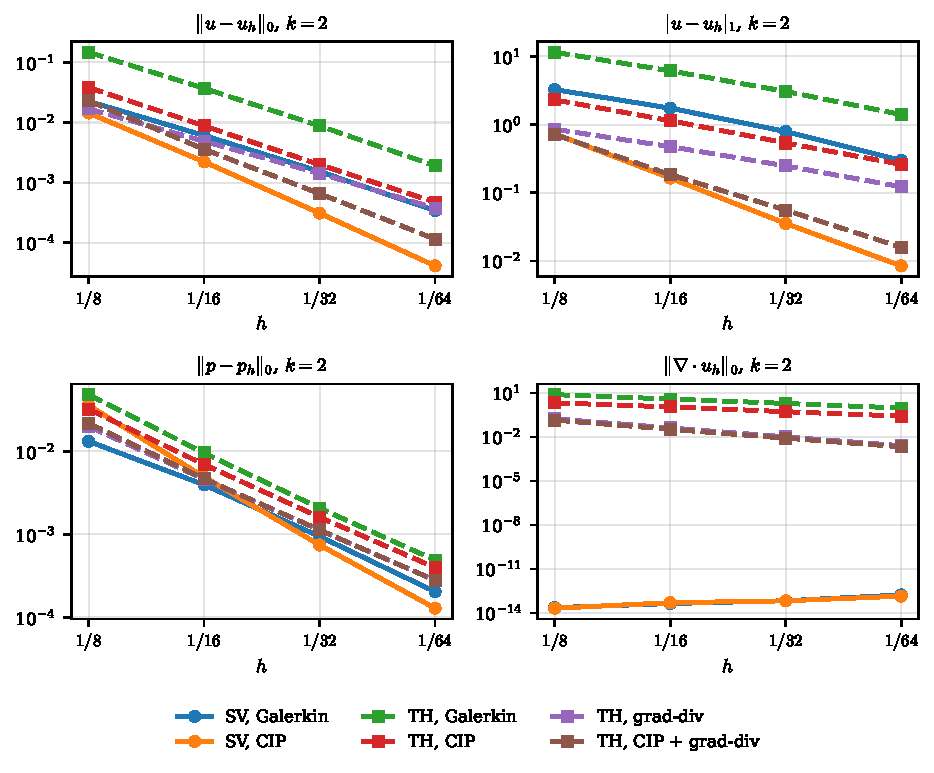
\includegraphics[width=\textwidth]{ex1_methods_errors.pdf}}{\torun{\fbox{\parbox{0.8\textwidth}{\centering\vspace{1cm}[\texttt{ex1\_methods\_errors.pdf}]\vspace{1cm}}}}}
  \caption{\new{Example 1, $k=2$, $\nu=10^{-6}$: velocity and pressure errors and divergence norm at $T$ against $h$ (solid: SV; dashed: TH).}}
  \label{fig:methods}
\end{figure}

\new{\paragraph{Convergence in time.} At $\nu=10^{-6}$ the vortex is quasi-steady and the temporal error is negligible; the time study therefore uses $\nu=0.05$, for which $e^{-5\pi^2\nu t}$ decays by a factor of about $3.4$ over $[0,T]$. On $n=16$ we use $N=10,20,40,80$ and a reference run with $N=320$ on the same mesh (Table~\ref{tab:time}, Figure~\ref{fig:time}). Both SV variants are second order, with velocity orders $2.10$, $2.05$ and $2.09$ and pressure orders $2.15$, $2.09$ and $2.11$ against the reference run; the stabilization leaves the temporal accuracy unchanged, the Galerkin and the CIP values agreeing to three digits.}

\begin{table}[htbp]
  \centering\small
  \caption{\new{Example 1, $k=2$, $n=16$, $\nu=0.05$: temporal error against the reference run with $N=320$ on the same mesh, at the largest $N$, and the observed orders in $N$ between consecutive runs.}}
  \label{tab:time}
  % filled 2026-10-20 from tg.tar: Taylor-Green time study, k=2, n=16, nu=0.05, T=0.5, reference N=320 (SV only in this version)
\begin{tabular}{lcccc}
\toprule
Method & $\|u_h^N-u_h^{\rm ref}\|_0$, $N=80$ & orders & $\|p_h^N-p_h^{\rm ref}\|_0$, $N=80$ & orders \\
\midrule
SV, Galerkin & 2.48e-5 & 2.10, 2.05, 2.09 & 4.58e-6 & 2.15, 2.09, 2.11 \\
SV, CIP & 2.48e-5 & 2.10, 2.05, 2.09 & 4.58e-6 & 2.15, 2.09, 2.11 \\
\bottomrule
\end{tabular}

\end{table}

\begin{figure}[htbp]
  \centering
  \IfFileExists{figures/ex1_time_convergence.pdf}{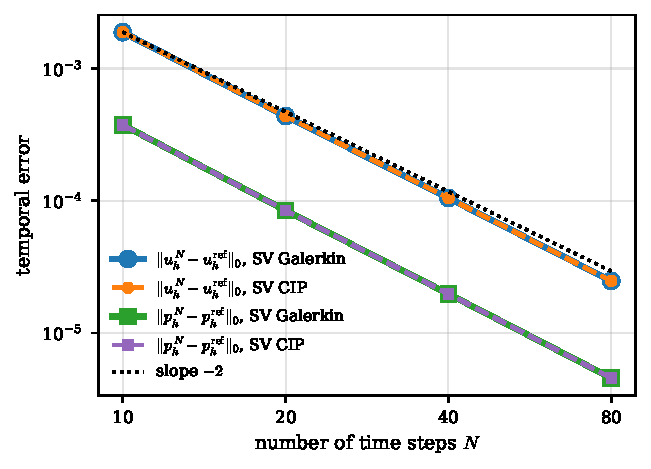
\includegraphics[width=0.62\textwidth]{ex1_time_convergence.pdf}}{\torun{\fbox{\parbox{0.8\textwidth}{\centering\vspace{1cm}[\texttt{ex1\_time\_convergence.pdf}: run \texttt{noslip\_study.py time}]\vspace{1cm}}}}}
  \caption{\new{Example 1, $k=2$, $n=16$, $\nu=0.05$: temporal error of velocity and pressure against the number of steps $N$. The dotted line has slope $-2$.}}
  \label{fig:time}
\end{figure}

\new{\paragraph{(E2) $\nu$-sweep.} Figure~\ref{fig:E2} shows $\|u(T)-u_h^N\|_0$ for $\nu=10^{-1},\dots,10^{-9}$, $k=2$, $n=16$, $32$ and $64$. For SV with CIP the error is bounded uniformly in $\nu$ and saturates at $2.2\cdot10^{-3}$, $3.1\cdot10^{-4}$ and $4.3\cdot10^{-5}$ for $\nu\lesssim10^{-6}$, that is, with orders $2.83$ and $2.87$. SV Galerkin saturates at errors $2.8$, $5.2$ and $9.8$ times larger, and its $H^1$ error ($1.80$, $0.89$ and $0.45$) is $11$ to $53$ times that of SV with CIP ($0.164$, $3.5\cdot10^{-2}$ and $8.5\cdot10^{-3}$). The SV saturation also lies below that of TH with grad-div ($4.90\cdot10^{-3}$, $1.45\cdot10^{-3}$ and $4.04\cdot10^{-4}$) by factors $2.2$, $4.6$ and $9.4$, growing under refinement, while for $\nu\ge10^{-2}$ the discretizations are comparable; the sharper separation appears in the pressure-robustness test (E3).}

\begin{figure}[htbp]
  \centering
  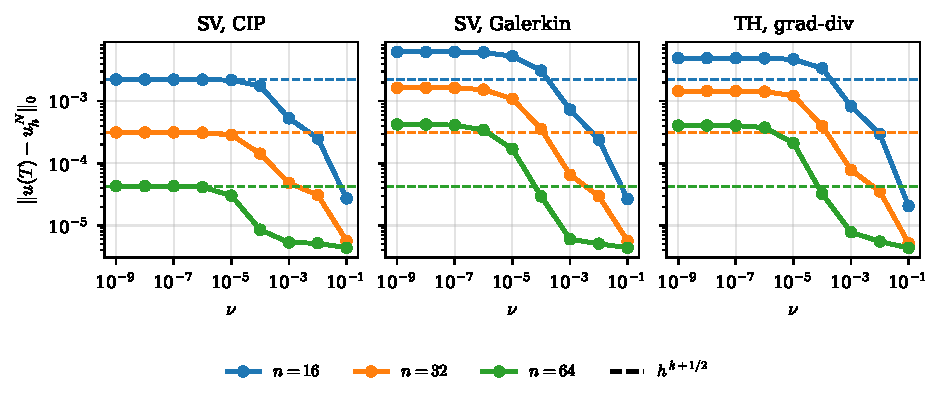
\includegraphics[width=\textwidth]{ex1_nu_sweep.pdf}
  \caption{\new{Example 1, (E2), $k=2$, $T=0.5$: $\|u(T)-u_h^N\|_0$ against $\nu$ on $n=16$, $32$ and $64$, for SV with CIP, SV Galerkin and TH with grad-div. Dashed: $Ch^{k+1/2}$, fitted to SV with CIP on the same mesh.}}
  \label{fig:E2}
\end{figure}

\new{\paragraph{(E3) Pressure robustness.} On $n=32$ with $\nu=10^{-6}$ we add the gradient force $R\nabla\phi$ with $R=10^2,10^4,10^6$ and compare with the run for $R=0$ (Table~\ref{tab:E3}). The SV velocity error is the same to all digits shown for every $R$, and the remaining drift is of order $10^{-11}R$, the solver tolerance applied to a right-hand side of size $R$; the SV pressure error grows in proportion to $\|p+R\phi\|_0$, as it must, while the velocity does not see the pressure. Every TH variant changes in proportion to $R$ or diverges: Galerkin diverges already at $R=10^2$, the stabilized variants carry drifts of order one at $R=10^2$ and of order ten at $R=10^4$, and only CIP with grad-div completes the run at $R=10^6$, with a drift of $2.6\cdot10^2$.}

\begin{table}[htbp]
  \centering\small
  \caption{\new{Example 1, (E3), $n=32$, $\nu=10^{-6}$, $k=2$: drift $\max|u_h^R-u_h^0|$ at $T$ and the velocity error. A dash means that the run diverged.}}
  \label{tab:E3}
  % filled 2026-10-20 from tg.tar: Taylor-Green pressure study, n=32, nu=1e-6, k=2, baseline R=0
\begin{tabular}{lcccc}
\toprule
Method & $R=10^2$ & $R=10^4$ & $R=10^6$ & $\|u-u_h\|_0$, $R=0\to10^6$ \\
\midrule
SV, Galerkin & 6.06e-9 & 2.30e-7 & 1.16e-5 & 1.53e-3 for all $R$ \\
SV, CIP & 6.87e-9 & 1.08e-6 & 5.31e-6 & 3.11e-4 for all $R$ \\
TH, Galerkin & -- & -- & -- & 8.77e-3 at $R=0$ \\
TH, CIP & 1.84 & 13.0 & -- & 1.99e-3 to 4.03 \\
TH, grad-div & 0.547 & 7.11 & -- & 1.42e-3 to 1.87 \\
TH, CIP + grad-div & 0.144 & 2.40 & 2.56e2 & 6.57e-4 to 105 \\
\bottomrule
\end{tabular}

\end{table}

\new{\paragraph{(E4) Role of the three CIP terms.} The analysis needs $S_2$ and $S_3$ only for the recovery step. To see whether they matter in practice, and whether the rate of Theorem~\ref{thm:velocity} survives without them, we run SV with $S_1$ only, $S_1+S_2$ and $S_1+S_2+S_3$, each with $(\delta_1,\delta_2,\delta_3)=s\,(10^{-1},10^{-2},10^{-3})$, $s\in\{0.1,1,10\}$, on $n=8,\dots,64$ (Table~\ref{tab:E4}). With these weights $S_3$ is much weaker than the other terms, so we add $S_1+S_2+S_3$ with $\delta_3=\delta_1$, which raises the third term to the weight of the first. The table also lists the TV ratio $\mathrm{TV}(\omega_h)/\mathrm{TV}(\omega)$ of the vorticity on a $128^2$ grid, the assembly time per step, and the number of nonzeros of the system matrix.}

\new{A geometric scaling $\delta_{j+1}/\delta_j=\beta$ is meant to give the three terms similar weight: each further derivative of a discrete function costs a factor $h^{-1}$, which the extra $h_F^2$ in $S_{j+1}$ cancels, and the factor $\beta$ compensates the larger constants of the higher derivatives; this example uses $\beta=10^{-1}$, the shear-layer runs of Table~\ref{tab:shearcip} use $\beta=10^{-2}$. Table~\ref{tab:E4scaling} checks the choice with the computed values of the terms with unit weights at $T$: a base $\beta$ is balanced when $S_{j+1}/S_j\approx\beta^{-1}$. All three terms couple only the degrees of freedom of the two elements sharing a face, so the stencil of the system matrix stays local; in the shear-layer runs of Table~\ref{tab:shearcip}, activating $S_2$ and $S_3$ fills in about $9\%$ more nonzeros within these blocks than $S_1$ alone ($340\,968$ against $313\,320$ at $n=16$), and $S_3$ adds none beyond $S_2$. In the double shear layer (Section~\ref{sec:shear}, $n=16$, Table~\ref{tab:shearcip}), $S_1$ alone gives TV ratios of $2.00$, $1.11$ and $0.73$ for $s=0.1,1,10$, against $1.87$, $0.96$ and $0.60$ with all three terms, and $S_1+S_2$ and $S_1+S_2+S_3$ agree to $0.01$ in every solution quantity; at $s=1$ and $s=10$, $S_1$ removes the over- and undershoots on its own, while at $s=0.1$ a vorticity undershoot of about $0.1$ remains for every combination of the terms.}

\new{On Example 1 (Table~\ref{tab:E4}), $S_1$ alone is at least as accurate as the full form and converges with the same or higher orders: at $s=1$ and $n=64$, $2.48\cdot10^{-5}$ $(3.14)$ against $4.14\cdot10^{-5}$ $(2.91)$, with the stabilization term of both at the predicted order $2.5$. The reweighted third term ($\delta_3=\delta_1$, a hundredfold increase) stays within a factor of about two of the full form in either direction, so $S_3$ remains numerically inactive at every tested weight; its role is the recovery step in the proof. The measured ratios in Table~\ref{tab:E4scaling} explain this: for the discrete error $e_h$, $S_2/S_1$ reaches $172$--$188$ at $s\ge1$, well above the balanced value $10$ of the base used here, so the second term carries $17$--$19$ times the weighted budget of the first, while $S_3/S_2$ stays between $0.03$ and $0.24$, so with $\delta_3=10^{-3}$ the third term contributes below one percent of the stabilization budget. The number of nonzeros grows by $5\%$ from $S_1$ to $S_1+S_2$ and not at all from $S_2$ to $S_3$, as in the shear-layer runs (Table~\ref{tab:shearcip}), and assembling the full form costs about $4.2$ times $S_1$ alone ($18$\,s against $4.3$\,s per step at $n=64$).}

\begin{table}[htbp]
  \centering\small
  \caption{\new{Example 1, (E4), SV, $k=2$, $\nu=10^{-6}$, $n=64$ (numbers in brackets: orders from $n=32$): CIP terms and strength $s$, $(\delta_1,\delta_2,\delta_3)=s\,(10^{-1},10^{-2},10^{-3})$ for the active terms. ``Stab.'' as in Table~\ref{tab:E1}; TV ratio of the vorticity on a $128^2$ grid; assembly time per step of the convection and CIP matrices.}}
  \label{tab:E4}
  % filled 2026-10-20 from tg.tar: Taylor-Green cip study, k=2, nu=1e-6, n=64 (orders from n=32)
\begin{tabular}{lrccccrr}
\toprule
Terms & $s$ & $\|u-u_h\|_0$ & $|u-u_h|_1$ & Stab. & TV ratio & ms/step & nonzeros \\
\midrule
Galerkin & -- & 3.44e-4 (2.16) & 0.298 (1.41) & -- & 2.02 & 1\,565 & 5\,670\,644 \\
$S_1$ & 0.1 & 1.65e-4 (2.21) & 3.65e-2 (1.40) & 1.05e-4 (2.22) & 1.02 & 4\,563 & 10\,327\,412 \\
$S_1+S_2$ & 0.1 & 1.39e-4 (2.36) & 3.06e-2 (1.63) & 1.72e-4 (2.43) & 1.01 & 7\,784 & 10\,864\,628 \\
$S_1+S_2+S_3$ & 0.1 & 1.40e-4 (2.37) & 3.07e-2 (1.60) & 1.72e-4 (2.43) & 1.01 & 18\,194 & 10\,864\,628 \\
$S_1+S_2+S_3$, $\delta_3=\delta_1$ & 0.1 & 1.50e-4 (2.45) & 3.34e-2 (1.59) & 1.91e-4 (2.70) & 1.01 & 18\,062 & 10\,864\,628 \\
$S_1$ & 1 & 2.48e-5 (3.14) & 8.00e-3 (1.98) & 1.03e-4 (2.48) & 1.00 & 4\,309 & 10\,327\,412 \\
$S_1+S_2$ & 1 & 4.20e-5 (2.91) & 8.59e-3 (2.18) & 4.57e-4 (2.49) & 1.00 & 7\,535 & 10\,864\,628 \\
$S_1+S_2+S_3$ & 1 & 4.14e-5 (2.91) & 8.45e-3 (2.07) & 4.57e-4 (2.50) & 1.00 & 18\,070 & 10\,864\,628 \\
$S_1+S_2+S_3$, $\delta_3=\delta_1$ & 1 & 3.39e-5 (3.22) & 7.54e-3 (2.35) & 5.09e-4 (2.82) & 1.00 & 18\,276 & 10\,864\,628 \\
$S_1$ & 10 & 5.02e-5 (2.70) & 1.09e-2 (1.96) & 2.78e-4 (2.55) & 1.00 & 4\,559 & 10\,327\,412 \\
$S_1+S_2$ & 10 & 1.42e-4 (2.86) & 2.05e-2 (2.15) & 1.44e-3 (2.50) & 1.00 & 7\,744 & 10\,864\,628 \\
$S_1+S_2+S_3$ & 10 & 1.33e-4 (2.86) & 1.89e-2 (2.07) & 1.44e-3 (2.50) & 1.00 & 17\,442 & 10\,864\,628 \\
$S_1+S_2+S_3$, $\delta_3=\delta_1$ & 10 & 2.51e-4 (3.43) & 7.76e-2 (1.44) & 2.43e-3 (2.94) & 1.03 & 18\,311 & 10\,864\,628 \\
\bottomrule
\end{tabular}

\end{table}

\begin{table}[htbp]
  \centering\small
  \caption{\new{Example 1, (E4), $n=64$: ratios of the CIP terms $S_j(w,w)$ with unit weights at $T$, for $w=u_h$ and $w=e_h=u_h-s_h$, in the run with all three terms.}}
  \label{tab:E4scaling}
  % filled 2026-10-20 from tg.tar: Taylor-Green raw S_j(w,w) with unit weights at T, k=2, n=64
\begin{tabular}{rcccc}
\toprule
$s$ & $S_2/S_1$ ($w=u_h$) & $S_3/S_2$ ($w=u_h$) & $S_2/S_1$ ($w=e_h$) & $S_3/S_2$ ($w=e_h$) \\
\midrule
0.1 & 5.3 & 0.24 & 24.7 & 0.08 \\
1 & 36.2 & 0.03 & 172 & 0.03 \\
10 & 46.0 & 0.03 & 188 & 0.03 \\
\bottomrule
\end{tabular}

\end{table}

\new{\paragraph{(E5) Time-step restriction.} With SV and CIP on $n=32$ we vary $\Delta t/h\in\{1/8,1/4,1/2,1,2,4\}$ and compare three normalizations of the stabilization: the original $\|\tu^{n+1}\|_{0,\infty}^{-1}$ of \eqref{eq:fully-discrete-scheme}, the one-sided $\max(10^{-2},\|\tu^{n+1}\|_{0,\infty})^{-1}$ used elsewhere in this section, and the clamped $N_{n+1}^{-1}$ of Remark~\ref{rem:clamp} with $u_{\min}$ half of $\min_t\|u(t)\|_{0,\infty}$ and $U_{\max}=1.25\max_t\|u(t)\|_{0,\infty}$ (Table~\ref{tab:E5}). A run counts as unbounded when $\|u_h^n\|_0$ exceeds $10\|u(t_n)\|_0$. The last column shows the range of $\|\tu^{n+1}\|_{0,\infty}$; the clamp acts only where this range leaves $[u_{\min},U_{\max}]$. No restriction is visible: every run is stable up to $\Delta t=4h$, and the three normalizations give identical errors to all digits shown. The error stays at the spatial level $3.11\cdot10^{-4}$ of Table~\ref{tab:E1} for $\Delta t\le h$ and even drops slightly for the largest steps ($2.20\cdot10^{-4}$ at $\Delta t=4h$), a cancellation within the spatial error level: the solution is quasi-steady at this $\nu$, so the $O(\Delta t^2)$ part is negligible even for the largest step. The range of $\|\tu^{n+1}\|_{0,\infty}$ is $[2.00,2.00]$ throughout --- the exact value $\|u(t)\|_{0,\infty}=2$ reproduced to three digits --- so it never leaves $[u_{\min},U_{\max}]$ and the clamps are never active.}

\begin{table}[htbp]
  \centering\small
  \caption{\new{Example 1, (E5), SV with CIP, $k=2$, $n=32$, $\nu=10^{-6}$: $\|u(T)-u_h^N\|_0$ for the three normalizations of the stabilization.}}
  \label{tab:E5}
  % filled 2026-10-20 from tg.tar: Taylor-Green dt study, SV with CIP, k=2, n=32, nu=1e-6
\begin{tabular}{rcccc}
\toprule
$\Delta t/h$ & original & one-sided & clamped & range of $\|\tilde u_h^{n+1}\|_{0,\infty}$ \\
\midrule
$1/8$ & 3.11e-4 & 3.11e-4 & 3.11e-4 & $[2.00,\,2.00]$ \\
$1/4$ & 3.11e-4 & 3.11e-4 & 3.11e-4 & $[2.00,\,2.00]$ \\
$1/2$ & 3.11e-4 & 3.11e-4 & 3.11e-4 & $[2.00,\,2.00]$ \\
1 & 3.08e-4 & 3.08e-4 & 3.08e-4 & $[2.00,\,2.00]$ \\
2 & 2.85e-4 & 2.85e-4 & 2.85e-4 & $[2.00,\,2.00]$ \\
4 & 2.20e-4 & 2.20e-4 & 2.20e-4 & $[2.00,\,2.00]$ \\
\bottomrule
\end{tabular}

\end{table}

\FloatBarrier

% ---------------------------------------------------------------------------
\subsection{Three-dimensional travelling vortex \new{(a variant of the analysed scheme)}}\label{sec:vortex3d}

\new{The vortex benchmark starts from a radially symmetric swirling flow, which is a steady solution of the incompressible Euler equations~\cite{MajdaBertozzi2002}. By Galilean invariance, the vortex can be carried along by a uniform background velocity $U_0$, as in Gresho's vortex~\cite{GreshoChan1990}. To obtain a Navier--Stokes solution, we move the viscous term into the forcing, $f=-\nu\Delta u$; the velocity--pressure pair is then an exact solution for every $\nu$.}

\new{In all cases the vortex centre starts at $c_0=\tfrac12\mathbf{1}$, the centre of the periodic domain, and moves with constant velocity $U_0$. Relative to the moving centre we use the coordinates}
\begin{equation}\label{eq:vortex}
  \xi_1 = x - \tfrac12 - U_{0,1}\,t, \qquad \xi_2 = y - \tfrac12 - U_{0,2}\,t,
  \qquad r^2 = \xi_1^2 + \xi_2^2,
\end{equation}
\new{where each $\xi_i$ is taken as its nearest periodic image in $[-\tfrac12,\tfrac12)$. The vortex axis is parallel to the $z$-axis, and the axial coordinate enters only through the transport. For a radial profile $g$, the swirl $A\,g(r^2)(-\xi_2,\xi_1)$ is balanced by the pressure gradient $\partial_rp=A^2r\,g(r^2)^2$, which gives an Euler solution; adding the viscous forcing above turns it into a Navier--Stokes solution. The amplitude $A$ is chosen so that the peak swirl speed is one. We take $\nu=10^{-7}$ and integrate up to $T=0.5$. The vortex is transported obliquely across the mesh, convection is of order one, and the pressure is not polynomial, so the test is demanding for all discretizations. The domain is the periodic unit cube, so the no-slip condition of the analysis does not hold; the results illustrate the behaviour of the method rather than test the theorems.}


\new{We stress that the three-dimensional computations in this subsection \emph{do not use the scheme analysed in this paper}: convection is treated fully explicitly, and the stabilization is a single gradient-jump CIP term rather than the three-term form $S$ (see below). Theorems~\ref{thm:stability}--\ref{thm:pressure} therefore do not apply. We include the results because they show pressure robustness and temporal accuracy of SV versus TH in three dimensions; we draw no conclusions about spatial convergence rates from the two SV meshes.}

\new{The three-dimensional test uses a columnar vortex with an axial jet of Batchelor type. Its profile is $q=\max\{0,1-r^2/R^2\}$ with $R=0.45$, $m=5$ and $J=\tfrac12$, the transport velocity is $U_0=(1,\tfrac12,\tfrac14)^\top$, and the amplitude is $A=\bigl(R\,\sigma^{1/2}(1-\sigma)^m\bigr)^{-1}\approx11.87$ with $\sigma=1/(2m+1)$:}
\begin{equation}\label{eq:vortex3d}
\begin{aligned}
  u(x,y,z,t) &= \begin{pmatrix} 1 - A\,\xi_2\,q^5 \\[2pt] \tfrac12 + A\,\xi_1\,q^5 \\[2pt]
                                \tfrac14 + J\,q^5 \end{pmatrix}, \qquad
  p(x,y,z,t) = -\frac{A^2R^2}{22}\,q^{11},\\
  f(x,y,z,t) &= -\frac{20\,\nu\,q^3}{R^2}
                \begin{pmatrix} -2A\,(2-3q)\,\xi_2 \\[2pt] 2A\,(2-3q)\,\xi_1 \\[2pt]
                                J\,(4-5q) \end{pmatrix}.
\end{aligned}
\end{equation}
\new{Since the profile vanishes for $r\ge R$, the field is exactly periodic. It belongs to $H^{m+1/2-\varepsilon}=H^{5.5-\varepsilon}$, and all three velocity components are nonzero.}

\new{For SV we use $P_3/P_2^{\rm disc}$, the lowest admissible degree in three dimensions ($k=d=3$), on Alfeld splits of Kuhn triangulations with $n=2,3,4$. TH uses $P_2/P_1$ on Kuhn meshes with $n=2,4,6,8$.}

\new{The three-dimensional implementation differs from the analysed scheme~\eqref{eq:fully-discrete-scheme} in two ways:}
\begin{itemize}
  \item Convection is treated \emph{fully explicitly}:
        $(({\tilde u}_h^{n+1}\cdot\nabla){\tilde u}_h^{n+1}, v_h)$,
        so the system matrix remains constant in time and no nonlinear solve is needed per step.
  \item The CIP stabilization uses \emph{gradient jumps} across interior facets:
        $\delta\sum_F h_F^2\int_F [\![\nabla u_h]\!]:[\![\nabla v_h]\!]
        \,\mathrm{d}s$, instead of the three-term form $S$.
\end{itemize}
\new{With explicit convection, Theorem~\ref{thm:stability} no longer applies, and the time step is subject to a CFL condition.}

\new{Table~\ref{tab:vortex3d} and Figures~\ref{fig:vortex3d-h}--\ref{fig:vortex3d-pressure} summarize the results.}

\new{Unstabilized SV diverges on the mesh $n=3$, and on $n=4$ its $H^1$ error is $26.7$; with explicit convection, Galerkin SV is simply not usable at this viscosity. SV with CIP ($\delta=10^{-3}$), on the other hand, stays stable on all meshes we tried. From $n=3$ to $n=4$ its observed orders are $2.73$ in $L^2$, $1.59$ in $H^1$ and $2.94$ for the pressure, but two coarse meshes are not enough to say anything about asymptotic rates, and Theorem~\ref{thm:velocity} does not cover this variant anyway. Unstabilized TH also does poorly: $|u-u_h|_1\approx10$ and $\|\nabla\cdot u_h\|_0\approx6$ stay large. The best TH results come from grad-div, which reaches an accuracy per degree of freedom comparable to SV with CIP at this moderate pressure.}

\new{For the temporal tests we use SV on $n=3$ and TH on $n=6$, with $N=40,80,160,320$ and a reference run with $N=1280$. All stabilized methods reach observed orders between $2.0$ and $2.15$ for velocity and pressure, so BDF2 keeps its accuracy in three dimensions as well. The pressure-robustness test (SV on $n=3$, TH on $n=6$) again separates the pairs. The SV velocity changes by at most $2\times10^{-10}$, even for $R=10^6$, where $\|p\|_0\approx5.6\times10^4$. For TH the change grows with $R$: with CIP and grad-div, $\max|u_h^R-u_h^0|$ increases from $6\times10^{-3}$ at $R=1$ to $0.65$ at $R=10^2$, and every TH run diverges for $R\ge10^4$.}

\new{Overall, the three-dimensional results agree with those of Example~1 (Section~\ref{sec:noslip}). They do not, however, show the rate $h^{k+1/2}$: the meshes needed to reach the asymptotic regime are beyond what our direct solvers can handle. Nor do they test the recovery property~\eqref{eq:potential-recovery}, on which the three-dimensional velocity estimate depends (Remark~\ref{rem:velocity}).}

\begin{table}[t]
  \centering\small
  \caption{Travelling vortex, $d = 3$: errors at time $T$
           (numbers in brackets: convergence order with respect to the previous mesh).
           A dash~(--) indicates that the computation diverged.}
  \label{tab:vortex3d}
  \begin{tabular}{lrrccc}
    \toprule
    Method & $n$ & dofs & $\|u-u_h\|_0$ & $|u-u_h|_1$ & $\|p-p_h\|_0$ \\
    \midrule
    SV $P_3$, Galerkin        & 3 &  9\,477 & --            & --            & --            \\
                              & 4 & 22\,464 & 2.0e-1        & 26.7          & 2.1e-1        \\
    SV $P_3$, CIP $10^{-3}$  & 3 &  9\,477 & 1.1e-1 (1.65) & 2.13 (1.07)   & 1.0e-1 (0.99) \\
                              & 4 & 22\,464 & 4.9e-2 (2.73) & 1.35 (1.59)   & 4.5e-2 (2.94) \\
    TH $P_2$, Galerkin        & 8 & 12\,288 & 2.1e-1 (1.73) & 9.80 (0.19)   & 1.2e-1 (1.35) \\
    TH $P_2$, grad-div        & 8 & 12\,288 & 4.2e-2 (2.47) & 1.31 (1.20)   & 4.5e-2 (2.28) \\
    \bottomrule
  \end{tabular}
\end{table}

\begin{figure}[t]
  \centering
  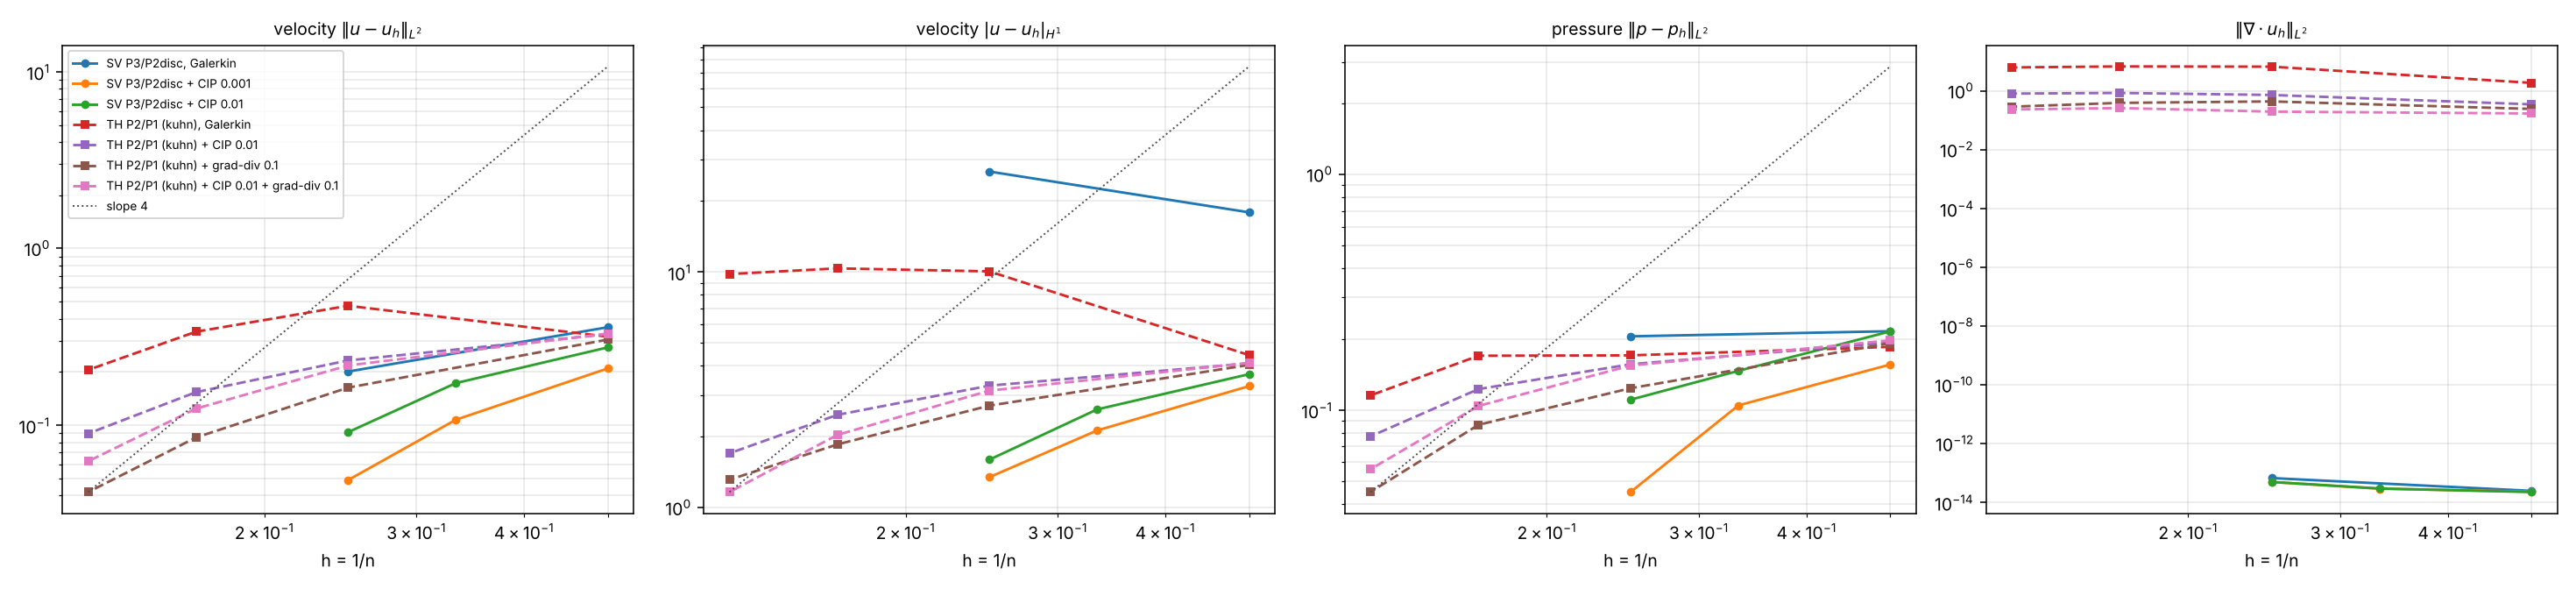
\includegraphics[width=\textwidth]{vortex3d_errors_vs_h.png}
  \caption{Travelling vortex, $d = 3$: errors at time $T$ against $h$
           (solid lines: SV $P_3$; dashed: TH $P_2$).
           The SV Galerkin run on $n = 3$ is absent because it diverged.}
  \label{fig:vortex3d-h}
\end{figure}

\begin{figure}[t]
  \centering
  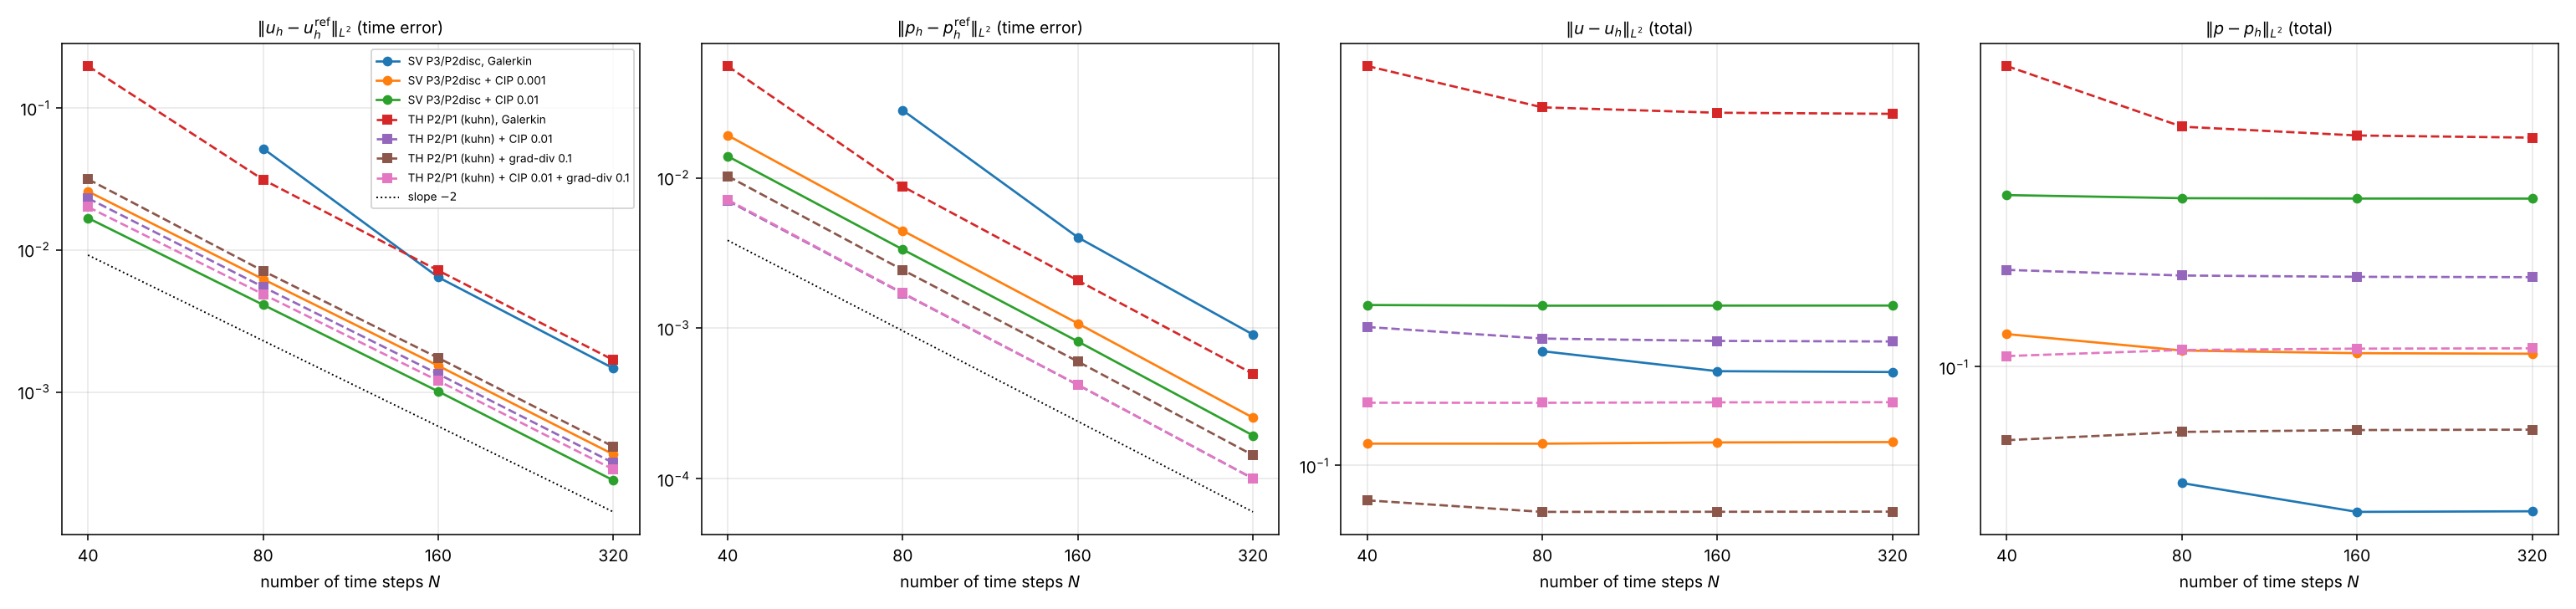
\includegraphics[width=\textwidth]{vortex3d_time_convergence.png}
  \caption{Travelling vortex, $d = 3$: time-discretization convergence against the number of
           steps $N$ (SV at $n = 3$, TH at $n = 6$; temporal error measured as the difference
           from the $N = 1280$ reference run). The dotted line shows slope $-2$.}
  \label{fig:vortex3d-time}
\end{figure}

\begin{figure}[t]
  \centering
  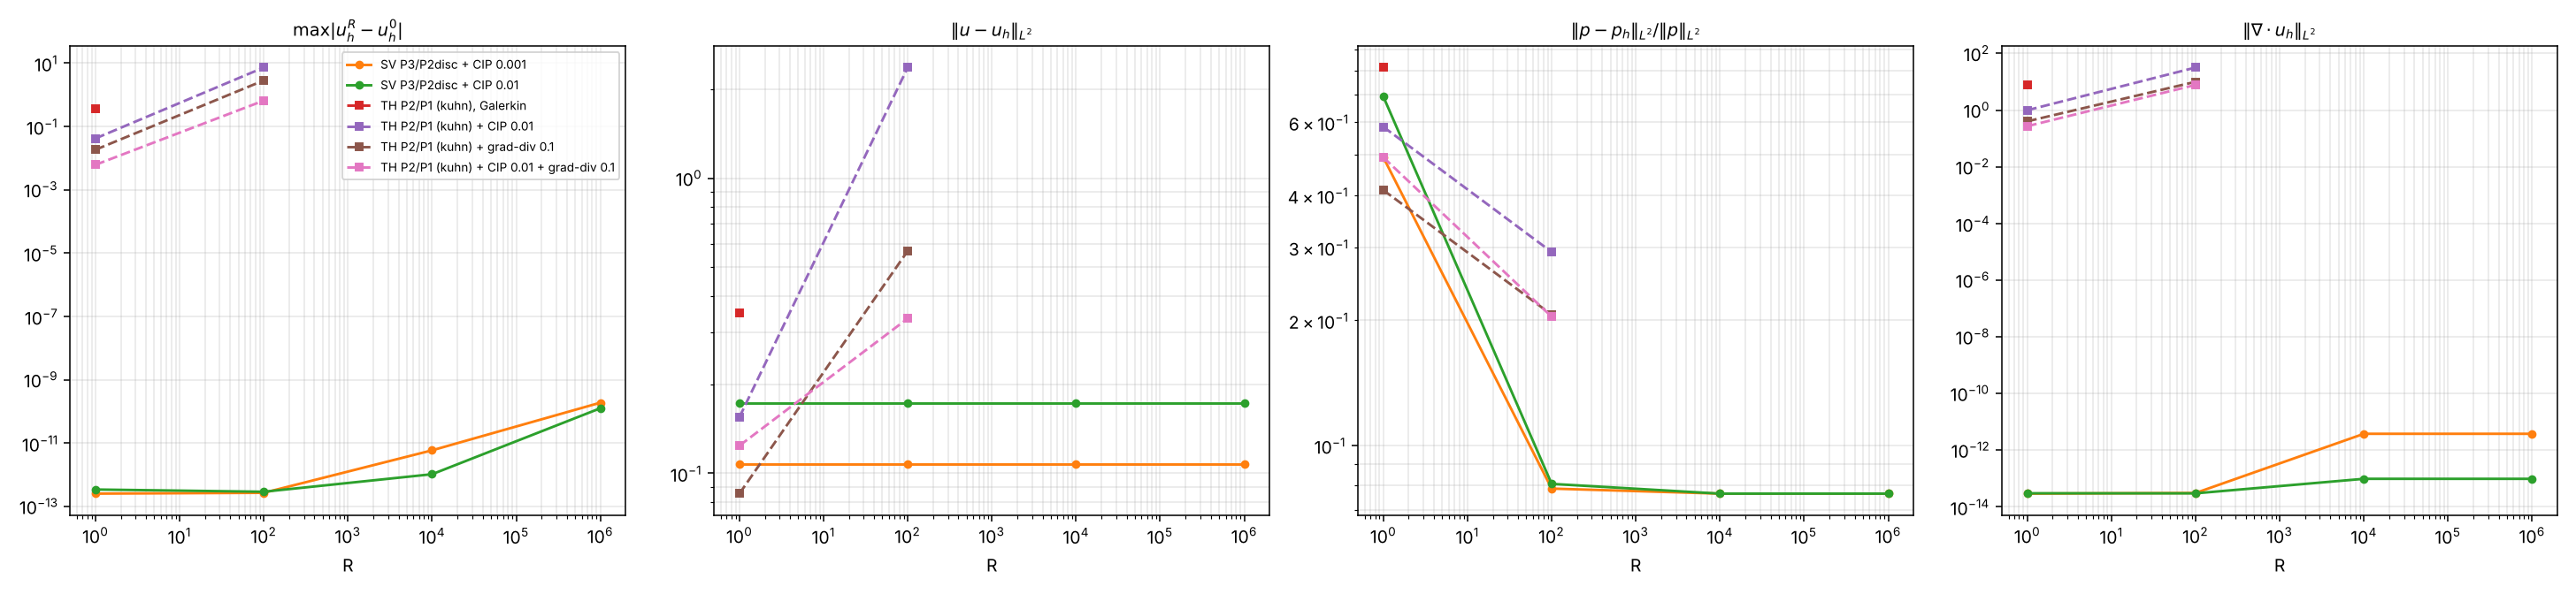
\includegraphics[width=\textwidth]{vortex3d_pressure_robustness.png}
  \caption{Travelling vortex, $d = 3$: pressure robustness
           (SV at $n = 3$, TH at $n = 6$). Missing points indicate divergence.}
  \label{fig:vortex3d-pressure}
\end{figure}

\FloatBarrier

% ---------------------------------------------------------------------------
\subsection{Spurious oscillations in an under-resolved double shear layer}%
\label{sec:shear}

\new{Our last test is the doubly periodic shear layer of Bell, Colella and Glaz~\cite{BellColellaGlaz1989}, a standard benchmark for spotting spurious vortical structures in under-resolved simulations~\cite{BrownMinion1995,MinionBrown1997}. On $(0,1)^2$ the initial velocity consists of two thin shear layers of opposite direction, perturbed by a small sinusoidal mode:}
\begin{equation}\label{eq:shear}
  u_0(x) =
  \begin{pmatrix}
    \tanh\!\bigl(\rho\,(\tfrac{1}{4} - |x_2 - \tfrac{1}{2}|)\bigr) \\[2pt]
    \delta\sin\!\bigl(2\pi(x_1 + \tfrac{1}{4})\bigr)
  \end{pmatrix}.
\end{equation}
\new{We take $\rho=80$, $\delta=0.05$ and $\nu=10^{-4}$. The layers roll up into two large vortices connected by thin braids. On coarse meshes, unstabilized methods tend to produce spurious secondary vortices along the braids, a well-known artefact that makes this problem a good diagnostic~\cite{BrownMinion1995}.}

\new{The reference solution is a fully dealiased pseudo-spectral computation with $512^2$ Fourier modes. We compare SV and TH with $k=2$ on the coarse mesh $n=16$ at $t=1$\new{, and repeat the comparison on $n=32$. Unlike the other tests, the time step here follows a CFL condition, $\Delta t\le0.2/(n\max|u_h^0|)$, rounded so that the output times are multiples of $\Delta t$: $\Delta t=10^{-2}$ on $n=16$ and $\Delta t=1/170\approx5.9\cdot10^{-3}$ on $n=32$}. Oscillations are quantified in two ways: by the overshoots and undershoots of the discrete vorticity $\omega_h$ beyond the reference range, normalized by $\max|\omega_{\rm ref}|$, and by the total variation ratio $\mathrm{TV}(\omega_h)/\mathrm{TV}(\omega_{\rm ref})$. A ratio above one means excess variation, a ratio below one means that the solution is smoother than the reference.}

\new{Unstabilized SV shows strong element-scale oscillations, with a total variation ratio of $4.3$ and a vorticity undershoot of $45\%$. Unstabilized TH is worse still: its total variation ratio is $6.3$, its divergence norm is $\|\nabla\cdot u_h\|_0=41$, and the velocity overshoots by $0.7$. For SV, CIP with unit strength ($s=1$) brings the total variation ratio down to $0.96$ and removes the over- and undershoots. At a tenth of this strength ($s=0.1$) oscillations are still visible, and much stronger CIP smears the vortex cores. For TH, grad-div matters as well: with CIP alone, velocity overshoots of $0.12$ remain, whereas grad-div alone removes the over- and undershoots and gives a ratio of $1.10$. Using both lowers the ratio to $0.74$.}

\new{Even with the oscillations gone, the relative vorticity error stays between $0.74$ and $0.95$ for all stabilized runs. This error is due to the poor resolution of the thin braids on the mesh $n=16$, not to oscillations; no stabilization can recover scales that the mesh cannot represent. \new{On $n=32$ (Table~\ref{tab:shear32}) the ranking is the same and the stabilized vorticity errors drop only to $0.66$--$0.74$, so the braids are still under-resolved. Two details differ: CIP with $s=0.1$ is now the most accurate SV run ($0.66$ against $0.69$ for $s=1$), and grad-div alone leaves a TV ratio of $1.47$ for TH.} We note that the CIP strength $s=1$ in Figure~\ref{fig:shear-showcase} was chosen afterwards, by comparing vorticity errors with the reference; it is a best case, not a recommended parameter value.}

\new{Table~\ref{tab:shearcip} isolates the contribution of the three CIP terms on the mesh $n=16$, for the strengths of experiment (E4) in Section~\ref{sec:noslip}. At $s=1$ and $s=10$, $S_1$ alone removes the over- and undershoots, and at unit strength it brings the TV ratio from $4.30$ down to $1.11$; adding $S_2$ lowers it to $0.97$, and $S_3$ changes no solution quantity by more than $0.01$. The price of the higher-order terms is assembly time: with the transport field, and hence all matrices, changing in every step, $S_1$ takes $52$\,ms per step to assemble, $S_1+S_2$ takes $92$\,ms and the full form $221$\,ms, against $17$\,ms for the Galerkin method. The stabilization is also dissipative: over $[0,1.5]$ the CIP terms account for about $21\%$ of the kinetic-energy loss at $s=0.1$, $35\%$ at $s=1$ and $57\%$ at $s=10$, with the viscous term contributing most of the rest. This over-dissipation at large $s$ is what smears the vortex cores, and it shows in the relative $L^2$ velocity error, which grows from $0.144$ (Galerkin) to $0.258$ ($s=1$) and $0.435$ ($s=10$) while the vorticity error improves.}


\begin{table}[t]
  \centering\small
  \caption{Double shear layer, $k = 2$, $n = 16$, $t = 1$.
           CIP strength $s$ means
           $(\delta_1,\delta_2,\delta_3) = s\,(10^{-2},10^{-4},10^{-6})$.
           The column labelled ``error'' is the relative $L^2$ error of $\omega_h$
           against the spectral reference.}
  \label{tab:shear}
  \begin{tabular}{lccccc}
    \toprule
    Method & TV ratio & $\omega$ over\,/\,under & $u$ over\,/\,under & error & $\|\nabla\cdot u_h\|_0$ \\
    \midrule
    SV, Galerkin           & 4.30 & 0.18\,/\,0.45 & 0\,/\,0       & 1.05 & 2e-10 \\
    SV, CIP $0.1$          & 1.87 & 0\,/\,0.10    & 0\,/\,0       & 0.76 & 2e-10 \\
    SV, CIP $1$            & 0.96 & 0\,/\,0       & 0\,/\,0       & 0.74 & 2e-10 \\
    TH, Galerkin           & 6.31 & 1.10\,/\,1.29 & 0.70\,/\,0.70 & 1.88 & 41    \\
    TH, CIP $1$            & 1.50 & 0\,/\,0.09    & 0.12\,/\,0.12 & 0.95 & 11    \\
    TH, grad-div           & 1.10 & 0\,/\,0       & 0\,/\,0       & 0.82 & 0.46  \\
    TH, CIP $1$ + grad-div & 0.74 & 0\,/\,0       & 0\,/\,0       & 0.79 & 0.46  \\
    \bottomrule
  \end{tabular}
\end{table}

\begin{table}[t]
  \centering\small
  \caption{\new{Double shear layer, $k=2$, $n=32$, $t=1$; columns as in Table~\ref{tab:shear}.}}
  \label{tab:shear32}
  \begin{tabular}{lccccc}
    \toprule
    Method & TV ratio & $\omega$ over\,/\,under & $u$ over\,/\,under & error & $\|\nabla\cdot u_h\|_0$ \\
    \midrule
    SV, Galerkin           & 2.49 & 0.20\,/\,0.38 & 0\,/\,0 & 0.74 & 9e-10 \\
    SV, CIP $0.1$          & 1.52 & 0.17\,/\,0.25 & 0\,/\,0 & 0.66 & 9e-10 \\
    SV, CIP $1$            & 1.02 & 0.01\,/\,0.07 & 0\,/\,0 & 0.69 & 9e-10 \\
    TH, Galerkin           & 3.01 & 0.83\,/\,0.33 & 0\,/\,0 & 0.88 & 7.2   \\
    TH, CIP $1$            & 1.21 & 0.44\,/\,0.01 & 0\,/\,0 & 0.73 & 5.0   \\
    TH, grad-div           & 1.47 & 0\,/\,0       & 0\,/\,0 & 0.73 & 0.20  \\
    TH, CIP $1$ + grad-div & 1.01 & 0\,/\,0       & 0\,/\,0 & 0.74 & 0.16  \\
    \bottomrule
  \end{tabular}
\end{table}

\begin{table}[t]
  \centering\small
  \caption{\new{Double shear layer, SV, $k=2$, $n=16$, $t=1$: role of the three CIP terms, experiment (E4) of Section~\ref{sec:noslip}. CIP strength $s$ as in Table~\ref{tab:shear}; ``$\omega$ error'' and ``$u$ error'' are the relative $L^2$ errors against the spectral reference; ``assembly'' is the time per step for the convection and CIP matrices, ``step'' the total time per step, and ``nnz'' the number of nonzeros of the system matrix.}}
  \label{tab:shearcip}
  \begin{tabular}{lcccccrrr}
    \toprule
    Terms & $s$ & TV ratio & $\omega$ over\,/\,under & $\omega$ error & $u$ error & assembly & step & nnz \\
    \midrule
    Galerkin      & --  & 4.30 & 0.18\,/\,0.45 & 1.05 & 0.144 &  17\,ms & 246\,ms & 178\,152 \\
    $S_1$         & 0.1 & 2.00 & 0\,/\,0.11    & 0.77 & 0.174 &  52\,ms & 316\,ms & 313\,320 \\
    $S_1+S_2$     & 0.1 & 1.88 & 0\,/\,0.10    & 0.76 & 0.176 &  93\,ms & 334\,ms & 340\,968 \\
    $S_1+S_2+S_3$ & 0.1 & 1.87 & 0\,/\,0.10    & 0.76 & 0.176 & 221\,ms & 456\,ms & 340\,968 \\
    $S_1$         & 1   & 1.11 & 0\,/\,0       & 0.75 & 0.265 &  52\,ms & 380\,ms & 313\,320 \\
    $S_1+S_2$     & 1   & 0.97 & 0\,/\,0       & 0.74 & 0.259 &  92\,ms & 385\,ms & 340\,968 \\
    $S_1+S_2+S_3$ & 1   & 0.96 & 0\,/\,0       & 0.74 & 0.258 & 221\,ms & 515\,ms & 340\,968 \\
    $S_1$         & 10  & 0.73 & 0\,/\,0       & 0.81 & 0.383 &  51\,ms & 499\,ms & 313\,320 \\
    $S_1+S_2$     & 10  & 0.61 & 0\,/\,0       & 0.84 & 0.435 &  92\,ms & 481\,ms & 340\,968 \\
    $S_1+S_2+S_3$ & 10  & 0.60 & 0\,/\,0       & 0.84 & 0.435 & 226\,ms & 608\,ms & 340\,968 \\
    \bottomrule
  \end{tabular}
\end{table}

\begin{figure}[t]
  \centering
  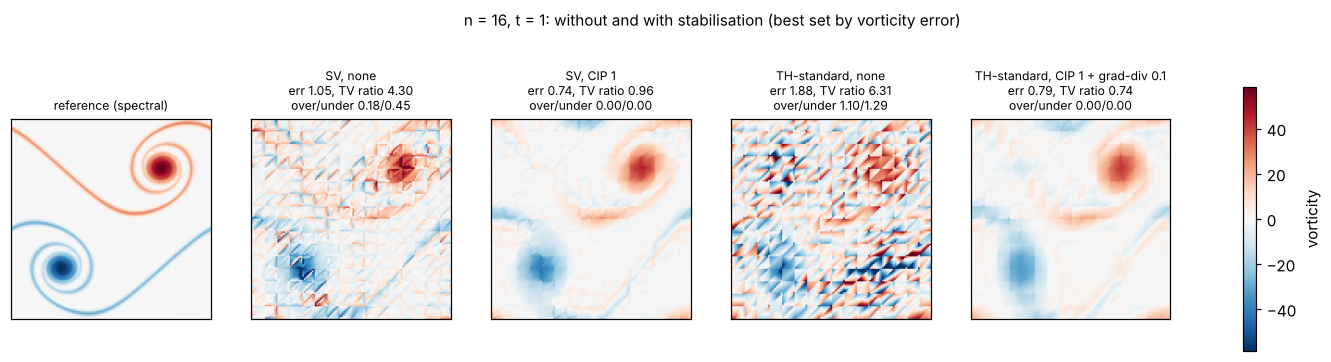
\includegraphics[width=\textwidth]{shear_vorticity_fields_n16.png}
  \caption{Double shear layer: vorticity fields at $t = 1$ on mesh $n = 16$, displayed on a
           common colour scale. From left to right: spectral reference, SV Galerkin, SV with
           the best CIP ($s = 1$), TH Galerkin, and TH with the best stabilization
           (CIP $s = 1$ and grad-div).}
  \label{fig:shear-showcase}
\end{figure}

\begin{figure}[t]
  \centering
  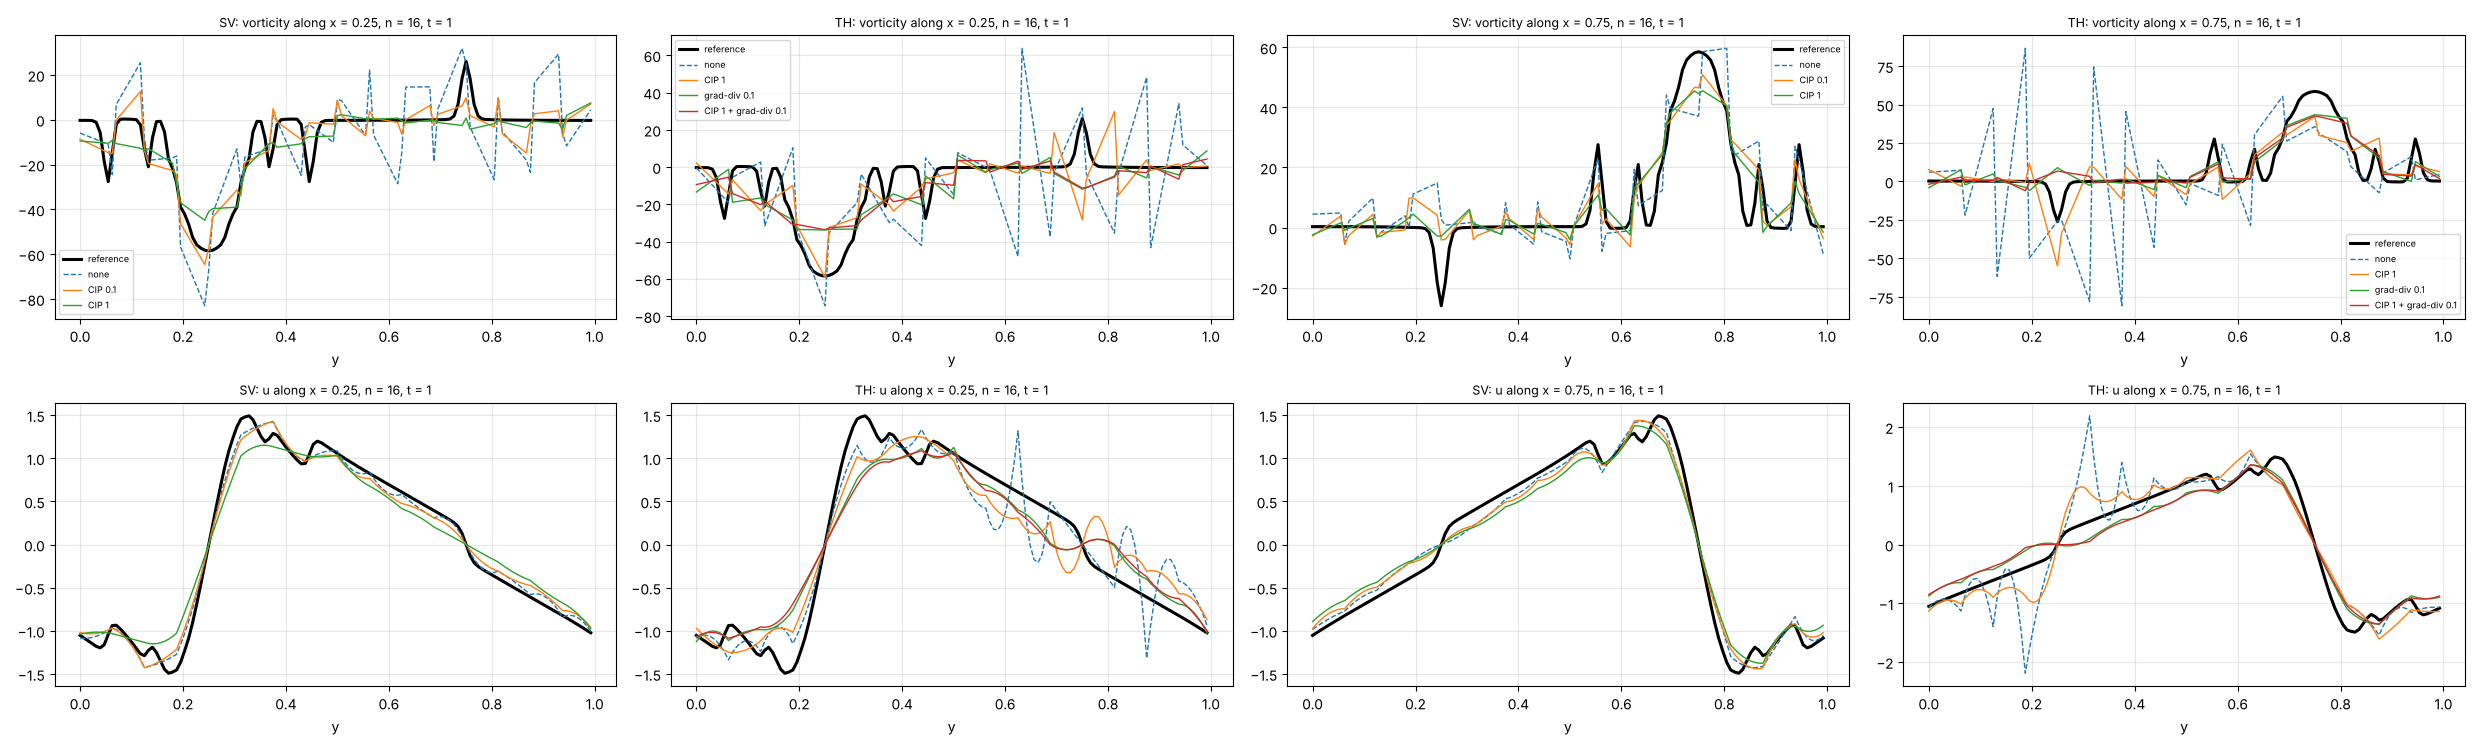
\includegraphics[width=\textwidth]{shear_profiles_n16.png}
  \caption{Double shear layer: one-dimensional profiles of $\omega$ and $u_1$ along the
           vertical lines $x_1 = 0.25$ and $x_1 = 0.75$ at $t = 1$, $n = 16$.}
  \label{fig:shear-cuts}
\end{figure}
\FloatBarrier


%=====================================================================
\fi
\appendix
\section{Discrete velocity time-derivative estimate}
This appendix explains the auxiliary estimate used in the pressure bound, namely
\begin{equation}\label{eq:time-derivative-goal}
\Delta t\sum_{n=1}^{N-1}\|\Dt e_u^{n+1}\|_{-1,h}^2\le C(h^{2k}+\Delta t^4),
\end{equation}
% REMOVED (rev): which is equivalent, up to the projection residual $\rho$, to hypothesis \eqref{eq:pressure-optimality-hypothesis}. We do not prove \eqref{eq:time-derivative-goal}. Lemma~\ref{lem:projected-time-derivative} proves its divergence-free projected version, and Proposition~\ref{prop:A1} derives from it a bound with an additional factor $h^{-2}$, which gives the suboptimal pressure bound of Theorem~\ref{thm:pressure}. The full estimate is the additional hypothesis of Corollary~\ref{cor:pressure-optimal}. Here $e_u^{n+1}=u^{n+1}-u_h^{n+1}$ denotes the total velocity error and $\|g\|_{-1,h}=\sup_{0\ne v_h\in\Vh}(g,v_h)/\|\nabla v_h\|_0$. We also use the projected divergence-free dual norm $\|g\|_{-1,h,\mathrm{div}}=\sup_{0\ne v_h\in\Vdivh}(g,v_h)/\|\nabla v_h\|_0$.
\new{which, up to the projection residual $\rho$, is the bound discussed in Remark~\ref{rem:optpressure}.} We do not prove \eqref{eq:time-derivative-goal}. Lemma~\ref{lem:projected-time-derivative} proves its divergence-free projected version, and Proposition~\ref{prop:A1} derives from it a bound with an additional factor $h^{-2}$, which gives \new{Theorem~\ref{thm:pressure}(iii)}. Here $e_u^{n+1}=u^{n+1}-u_h^{n+1}$ denotes the total velocity error and $\|g\|_{-1,h}=\sup_{0\ne v_h\in\Vh}(g,v_h)/\|\nabla v_h\|_0$. We also use the projected divergence-free dual norm $\|g\|_{-1,h,\mathrm{div}}=\sup_{0\ne v_h\in\Vdivh}(g,v_h)/\|\nabla v_h\|_0$.

Subtract the fully discrete momentum equation in \eqref{eq:fully-discrete-scheme} from the exact momentum equation in \eqref{eq:weak-form} at $t_{n+1}$. After adding and subtracting the BDF2 derivative of the exact solution, one obtains, for every $v_h\in\Vh$,
\begin{equation}\label{eq:time-derivative-error-identity}
(\Dt e_u^{n+1},v_h)=(\tau^{n+1},v_h)-\nu(\nabla e_u^{n+1},\nabla v_h)+(p^{n+1}-p_h^{n+1},\nabla\cdot v_h)-C^{n+1}(v_h)+\Simex^{n+1}(u_h^{n+1},v_h),
\end{equation}
where
\[
C^{n+1}(v_h)=(u^{n+1}\cdot\nabla u^{n+1},v_h)-((\tu^{n+1}\cdot\nabla)u_h^{n+1},v_h),\qquad
\tau^{n+1}=\Dt u^{n+1}-\partial_tu(t_{n+1}).
\]

The pressure term is the obstruction to a completely pressure-robust estimate of the full norm $\|\Dt e_u^{n+1}\|_{-1,h}$, because the supremum is taken over all of $\Vh$, not only over the discretely divergence-free subspace. Indeed,
\[
|(p^{n+1}-p_h^{n+1},\nabla\cdot v_h)|\le\sqrt d\,\|p^{n+1}-p_h^{n+1}\|_0\|\nabla v_h\|_0,
\]
so the full dual norm necessarily contains a pressure-error contribution. However, this obstruction disappears after projection onto $\Vdivh$.

The BDF2 consistency error has the Peano-kernel representation
\[
\tau^{n+1}=\frac1{2\Delta t}\int_{t_{n-1}}^{t_{n+1}}K_n(s)\,\partial_{ttt}u(s)\,\dd s,\qquad |K_n(s)|\le C\Delta t^2.
\]
Thus, if $\partial_{ttt}u\in L^2(0,T;H^{-1})$,
\begin{equation}\label{eq:bdf2-consistency-negative-norm}
\Delta t\sum_{n=1}^{N-1}\|\tau^{n+1}\|_{H^{-1}}^2\le C\Delta t^4\|\partial_{ttt}u\|_{L^2(0,T;H^{-1})}^2.
\end{equation}
The viscous part is controlled by the velocity estimate together with the projection estimate for $\nabla\eta$:
\begin{equation}\label{eq:viscous-negative-norm-bound}
\Delta t\sum_{n=1}^{N-1}\nu^2\|\nabla e_u^{n+1}\|_0^2\le C\Delta t\sum_{n=1}^{N-1}\big(\nu^2\|\nabla e_h^{n+1}\|_0^2+\nu^2\|\nabla\eta^{n+1}\|_0^2\big)\le C(h^{2k}+\Delta t^4).
\end{equation}
The convective and stabilization residuals satisfy, as in the proof of Theorem~\ref{thm:pressure},
\begin{equation}\label{eq:convective-stabilization-residual-bound}
\Delta t\sum_{n=1}^{N-1}\|R^{n+1}_{\mathrm{conv}}\|_{-1,h}^2+\Delta t\sum_{n=1}^{N-1}\|R^{n+1}_{\mathrm{stab}}\|_{-1,h}^2\le C(h^{2k}+\Delta t^4).
\end{equation}
\begin{lemma}[Projected time-derivative estimate]\label{lem:projected-time-derivative}
The discrete time derivative of the velocity error satisfies
\begin{equation}\label{eq:projected-time-derivative-bound}
\Delta t\sum_{n=1}^{N-1}\|\Dt e_u^{n+1}\|_{-1,h,\mathrm{div}}^2\le C(h^{2k}+\Delta t^4).
\end{equation}
\end{lemma}
\begin{proof}
Restrict \eqref{eq:time-derivative-error-identity} to $v_h\in\Vdivh$. Then $(p^{n+1}-p_h^{n+1},\nabla\cdot v_h)=0$, so the pressure residual vanishes and
\[\frac{|(\Dt e_u^{n+1},v_h)|}{\|\nabla v_h\|_0}\le C\|\tau^{n+1}\|_{H^{-1}}+C\nu\|\nabla e_u^{n+1}\|_0+C\|R_{\mathrm{conv}}^{n+1}\|_{-1,h}+C\|R_{\mathrm{stab}}^{n+1}\|_{-1,h}.\]
Taking the supremum over $\Vdivh$, squaring, multiplying by $\Delta t$, summing over $n$, and applying \eqref{eq:bdf2-consistency-negative-norm}, \eqref{eq:viscous-negative-norm-bound}, and \eqref{eq:convective-stabilization-residual-bound} proves \eqref{eq:projected-time-derivative-bound}.
\end{proof}
The preceding lemma is pressure-robust, but it controls only the divergence-free component of the dual norm.

\begin{proposition}\label{prop:A1}
Under the hypotheses of Theorem~\ref{thm:velocity},
\[\Delta t\sum_{n=1}^{N-1}\|\Dt e_h^{n+1}\|_{-1,h}^2\le C\,h^{-2}(h^{2k}+\Delta t^4),\]\[\text{hence}\qquad\Big(\Delta t\sum_{n=1}^{N-1}\|p^{n+1}-p_h^{n+1}\|_0^2\Big)^{1/2}\le C\Big(h^{k-1}+\frac{\Delta t^2}{h}\Big).\]
\end{proposition}
\begin{proof}
Since $e_h=\eta-e_u$, $g:=\Dt e_h^{n+1}=\rho^{n+1}-\Dt e_u^{n+1}\in\Vdivh$. (i)~For $g\in\Vdivh$ we may take $v_h=g$ in the divergence-free dual norm:
\[
\|g\|_0^2\le\|g\|_{-1,h,\mathrm{div}}\|\nabla g\|_0\le C_{\mathrm{inv}}h^{-1}\|g\|_{-1,h,\mathrm{div}}\|g\|_0,
\qquad\text{so}\qquad
\|g\|_0\le C_{\mathrm{inv}}h^{-1}\|g\|_{-1,h,\mathrm{div}}.
\]
(ii)~Trivially $\|g\|_{-1,h}\le C_P\|g\|_0$ (Poincar\'e). (iii)
\[
\|g\|_{-1,h,\mathrm{div}}\le\|\rho^{n+1}\|_{-1,h}+\|\Dt e_u^{n+1}\|_{-1,h,\mathrm{div}}.
\]
Squaring, summing, and using Lemma~\ref{lem:projected-time-derivative} and $\Delta t\sum\|\rho^{n+1}\|_0^2\le Ch^{2k+2}$ gives the first claim. For the second, $\|\Dt e_u\|_{-1,h}\le\|\rho\|_{-1,h}+\|\Dt e_h\|_{-1,h}$ is inserted in the cumulative bound of Theorem~\ref{thm:pressure}, whose remaining terms are $O(h^{2k}+\Delta t^4)$.
\end{proof}
% REMOVED (rev): \begin{remark}
% REMOVED (rev): The loss of one power of $h$ is an artefact of the inverse inequality in (i). Removing it, i.e.\ proving \eqref{eq:pressure-optimality-hypothesis}, requires an $H^1$-level estimate: test the error equation with $\Dt e_h^{n+1}\in\Vdivh$ and use $G$-stability of BDF2 for $(\nabla e_h,\nabla\Dt e_h)$. This needs $L^2$-norm control of the consistency residuals of the nonlinear and CIP terms, which are not available from the present analysis; this is not carried out here. A $G$-stability bound for first-order differences of BDF schemes that may serve this purpose was recently proposed in \cite{GAJN25}.
% REMOVED (rev): \end{remark}
% (Remark moved to Section 4 as Remark rem:optpressure.)



\begin{thebibliography}{99}\small
\bibitem{ABBGLM21} N.~Ahmed, G.~R.~Barrenechea, E.~Burman, J.~Guzm\'an, A.~Linke, C.~Merdon, A pressure-robust discretization of Oseen's equation using stabilization in the vorticity equation, \emph{SIAM J. Numer. Anal.} 59(5):2746--2774, 2021.
\bibitem{AQ92} D.~N.~Arnold, J.~Qin, Quadratic velocity/linear pressure Stokes elements, in: \emph{Advances in Computer Methods for Partial Differential Equations VII}, IMACS, 1992, pp.~28--34.
\bibitem{BBCG24} G.~R.~Barrenechea, E.~Burman, E.~C\'aceres, J.~Guzm\'an, Continuous interior penalty stabilization for divergence-free finite element methods, \emph{IMA J. Numer. Anal.} 44(2):980--1002, 2024.
\bibitem{BBG20} G.~R.~Barrenechea, E.~Burman, J.~Guzm\'an, Well-posedness and $H(\mathrm{div})$-conforming finite element approximation of a linearised model for inviscid incompressible flow, \emph{Math. Models Methods Appl. Sci.} 30(5):847--865, 2020.
\bibitem{BDV24} L.~Beir\~ao da Veiga, F.~Dassi, G.~Vacca, Pressure robust SUPG-stabilized finite elements for the unsteady Navier--Stokes equation, \emph{IMA J. Numer. Anal.} 44(2):710--750, 2024; Erratum, 44(6):3815--3819, 2024.
\bibitem{BDDG25} L.~Beir\~ao da Veiga, F.~Dassi, S.~G\'omez, Fully and semi-implicit robust space--time DG methods for the incompressible Navier--Stokes equations, arXiv:2502.19035, 2025.
\bibitem{BDDHR25} L.~Beir\~ao da Veiga, D.~A.~Di~Pietro, J.~Droniou, K.~B.~Haile, T.~J.~Radley, A Reynolds-semirobust method with hybrid velocity and pressure for the unsteady incompressible Navier--Stokes equations, \emph{SIAM J. Numer. Anal.} 63(6):2317--2342, 2025.
\bibitem{BF07} E.~Burman, M.~A.~Fern\'andez, Continuous interior penalty finite element method for the time-dependent Navier--Stokes equations: space discretization and convergence, \emph{Numer. Math.} 107(1):39--77, 2007.
\bibitem{BFH06} E.~Burman, M.~A.~Fern\'andez, P.~Hansbo, Continuous interior penalty finite element method for Oseen's equations, \emph{SIAM J. Numer. Anal.} 44(3):1248--1274, 2006.
\bibitem{BG20} E.~Burman, J.~Guzm\'an, Implicit-explicit multistep formulations for finite element discretisations using continuous interior penalty, arXiv:2012.05727, 2020.
\bibitem{CM10} M.~Costabel, A.~McIntosh, On Bogovski\u{\i} and regularized Poincar\'e integral operators for de Rham complexes on Lipschitz domains, \emph{Math. Z.} 265(2):297--320, 2010.
\bibitem{dFGAJN18} J.~de~Frutos, B.~Garc\'ia-Archilla, V.~John, J.~Novo, Analysis of the grad-div stabilization for the time-dependent Navier--Stokes equations with inf-sup stable finite elements, \emph{Adv. Comput. Math.} 44(1):195--225, 2018.
\bibitem{FGN20} G.~Fu, J.~Guzm\'an, M.~Neilan, Exact smooth piecewise polynomial sequences on Alfeld splits, \emph{Math. Comp.} 89(323):1059--1091, 2020.
\bibitem{GAJN25} B.~Garc\'ia-Archilla, V.~John, J.~Novo, Error analysis of BDF schemes for the evolutionary incompressible Navier--Stokes equations, arXiv:2506.16917, 2025.
\bibitem{GAN23} B.~Garc\'ia-Archilla, J.~Novo, Robust error bounds for the Navier--Stokes equations using implicit-explicit second order BDF method with variable steps, \emph{IMA J. Numer. Anal.} 43(5):2892--2933, 2023.
\bibitem{GAN25} B.~Garc\'ia-Archilla, J.~Novo, Pressure and convection robust bounds for continuous interior penalty divergence-free finite element methods for the incompressible Navier--Stokes equations, \emph{IMA J. Numer. Anal.} 45(1):163--187, 2025 (arXiv:2303.10992; equation and lemma numbers refer to the arXiv version).
\bibitem{GJN21} B.~Garc\'ia-Archilla, V.~John, J.~Novo, On the convergence order of the finite element error in the kinetic energy for high Reynolds number incompressible flows, \emph{Comput. Methods Appl. Mech. Engrg.} 385:114032, 2021.
\bibitem{GN18} J.~Guzm\'an, M.~Neilan, Inf-sup stable finite elements on barycentric refinements producing divergence-free approximations in arbitrary dimensions, \emph{SIAM J. Numer. Anal.} 56(5):2826--2844, 2018.
\bibitem{GSS17} J.~Guzm\'an, C.-W.~Shu, F.~A.~Sequeira, $H(\mathrm{div})$ conforming and DG methods for incompressible Euler's equations, \emph{IMA J. Numer. Anal.} 37(4):1733--1771, 2017.
\bibitem{HH21} Y.~Han, Y.~Hou, Robust error analysis of $H(\mathrm{div})$-conforming DG method for the time-dependent incompressible Navier--Stokes equations, \emph{J. Comput. Appl. Math.} 390:113365, 2021.
\bibitem{JLMNR17} V.~John, A.~Linke, C.~Merdon, M.~Neilan, L.~G.~Rebholz, On the divergence constraint in mixed finite element methods for incompressible flows, \emph{SIAM Rev.} 59(3):492--544, 2017.
\bibitem{SL17} P.~W.~Schroeder, G.~Lube, Pressure-robust analysis of divergence-free and conforming FEM for evolutionary incompressible Navier--Stokes flows, \emph{J. Numer. Math.} 25(4):249--276, 2017.
\bibitem{Zha05} S.~Zhang, A new family of stable mixed finite elements for the 3D Stokes equations, \emph{Math. Comp.} 74(250):543--554, 2005.

\bibitem{MajdaBertozzi2002} A.~J.~Majda and A.~L.~Bertozzi, \emph{Vorticity and Incompressible Flow}, Cambridge University Press, Cambridge, 2002.
\bibitem{GreshoChan1990} P.~M.~Gresho and S.~T.~Chan, On the theory of semi-implicit projection methods for viscous incompressible flow and its implementation via a finite element method that also introduces a nearly consistent mass matrix. Part 2: Implementation, \emph{Int. J. Numer. Methods Fluids} 11(5):621--659, 1990.
\bibitem{BellColellaGlaz1989} J.~B.~Bell, J.~Colella, and H.~M.~Glaz, A second-order projection method for the incompressible Navier--Stokes equations, \emph{J. Comput. Phys.} 85(2):257--283, 1989.
\bibitem{BrownMinion1995} D.~L.~Brown and M.~L.~Minion, Performance of under-resolved two-dimensional incompressible flow simulations, \emph{J. Comput. Phys.} 122(1):165--183, 1995.
\bibitem{MinionBrown1997} M.~L.~Minion and D.~L.~Brown, Performance of under-resolved two-dimensional incompressible flow simulations, II, \emph{J. Comput. Phys.} 138(2):734--765, 1997.
\new{\bibitem{GR86} V.~Girault, P.-A.~Raviart, \emph{Finite Element Methods for Navier--Stokes Equations}, Springer, Berlin, 1986.}
\new{\bibitem{HW96} E.~Hairer, G.~Wanner, \emph{Solving Ordinary Differential Equations II}, 2nd ed., Springer, Berlin, 1996.}
\new{\bibitem{Joh16} V.~John, \emph{Finite Element Methods for Incompressible Flow Problems}, Springer, Cham, 2016.}
\new{\bibitem{BH04} E.~Burman, P.~Hansbo, Edge stabilization for Galerkin approximations of convection--diffusion--reaction problems, \emph{Comput. Methods Appl. Mech. Engrg.} 193(15--16):1437--1453, 2004.}
\new{\bibitem{GLS19} N.~R.~Gauger, A.~Linke, P.~W.~Schroeder, On high-order pressure-robust space discretisations, their advantages for incompressible high Reynolds number generalised Beltrami flows and beyond, \emph{SMAI J. Comput. Math.} 5:89--129, 2019.}
\new{\bibitem{Lin14} A.~Linke, On the role of the Helmholtz decomposition in mixed methods for incompressible flows and a new variational crime, \emph{Comput. Methods Appl. Mech. Engrg.} 268:782--800, 2014.}
\new{\bibitem{LM16} A.~Linke, C.~Merdon, Pressure-robustness and discrete Helmholtz projectors in mixed finite element methods for the incompressible Navier--Stokes equations, \emph{Comput. Methods Appl. Mech. Engrg.} 311:304--326, 2016.}
\new{\bibitem{SV85} L.~R.~Scott, M.~Vogelius, Norm estimates for a maximal right inverse of the divergence operator in spaces of piecewise polynomials, \emph{RAIRO Mod\'el. Math. Anal. Num\'er.} 19(1):111--143, 1985.}
\end{thebibliography}
\end{document}